\chapter{Segmentation}


\section{Semantic segmentation}

\begin{description}
    \item[Semantic segmentation] \marginnote{Semantic segmentation}
        Given an input image, output a category for each pixel.

    \item[Pixel-wise IoU] \marginnote{Pixel-wise IoU}
        IoU generalized to pixel-wise segmentation masks. Given a class $c$, the ground-truths $y^{(i)}$, and predictions $\hat{y}^{(i)}$, the IoU w.r.t. $c$ is computed as follows:
        \[
            \begin{gathered}
                TP_c = \sum_{i=1} | \text{pixels $(u, v): y_{(u, v)}^{(i)} = c \land \hat{y}_{(u, v)}^{(i)} = c$} | \\
                \texttt{IoU}_c = \frac{TP_c}{\sum_{i=1} \left( | (u, v): \hat{y}_{(u, v)}^{(i)} = c | + | (u, v): y_{(u, v)}^{(i)} = c | \right) - TP_c}
            \end{gathered}
        \]

        The mean IoU is computed as:
        \[ \texttt{mIoU} = \frac{1}{C} \sum_{c=1}^{C} \texttt{IoU}_c \]


        \begin{remark}
            Mean IoU is not strictly correlated to human's perception of segmentation. A small gain in \texttt{mIoU} might correspond to a large visual improvement.
        \end{remark}
\end{description}


\subsection{Kinect human pose estimation}

\begin{description}
    \item[Human pose detection] \marginnote{Human pose detection}
        Task of detecting the position and orientation of a person.

    \item[Pipeline]
        Kinect pose detection is done in three phases:
        \begin{enumerate}
            \item Capture a depth image and remove the background to obtain the depth map of a person.
            \item Classify each pixel into a body part.
            \item Determine the position of the joints (i.e., skeleton) by finding local modes (i.e., center of mass).
        \end{enumerate}

    \item[Synthetic annotated data] \marginnote{Synthetic annotated data}
        The data used to create the model is artificially generated. $100$k poses were captured using motion capture devices. Then, different mock-up body models (for which the ground-truth is known) were simulated and recorded through a virtual camera with the same intrinsic parameters of the Kinect camera. This allows to obtain robustness with different body and clothing shapes.

        \begin{remark}
            The workflow of the original paper consists of iteratively training the model and creating new training data for poses that the current model struggles on.
        \end{remark}

        \begin{figure}[H]
            \centering
            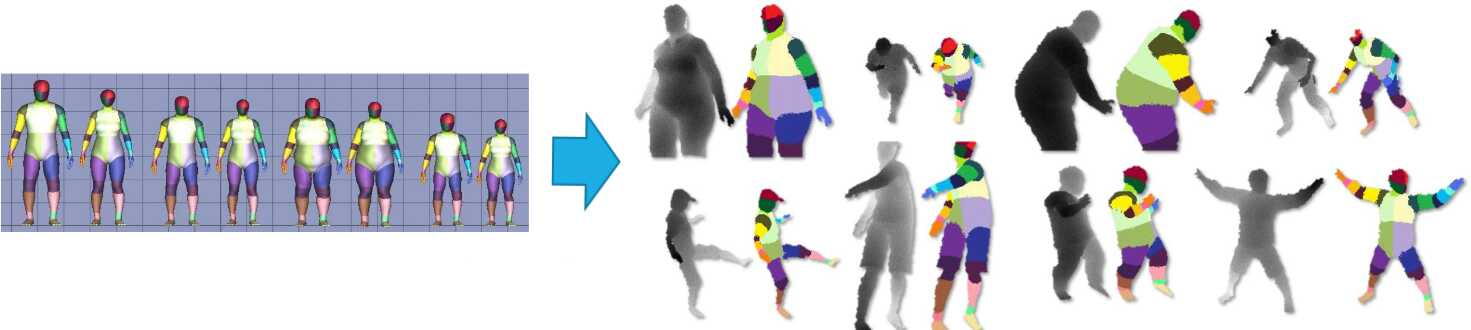
\includegraphics[width=0.75\linewidth]{./img/motion_data.jpg}
        \end{figure}

    \item[Depth comparison features] \marginnote{Depth comparison features}
        Given a depth image $D$ and the offsets $\theta = (\Delta p, \Delta n)$, each pixel $x$ of $D$ produces a feature as follows:
        \[ f(x; D, (\Delta p, \Delta n)) = D\left[ x + \frac{\Delta p}{D[x]} \right] - D\left[ x + \frac{\Delta n}{D[x]} \right] \]
        In other words, each $x$ is described by the difference in depth between two points offset from $x$. The depth at background pixels is a large positive number.

        \begin{remark}
            As real-time processing is required, this approach allows to quickly compute features to discriminate parts of the body. However, it does not always produce a correct response.
        \end{remark}

        \begin{figure}[H]
            \centering
            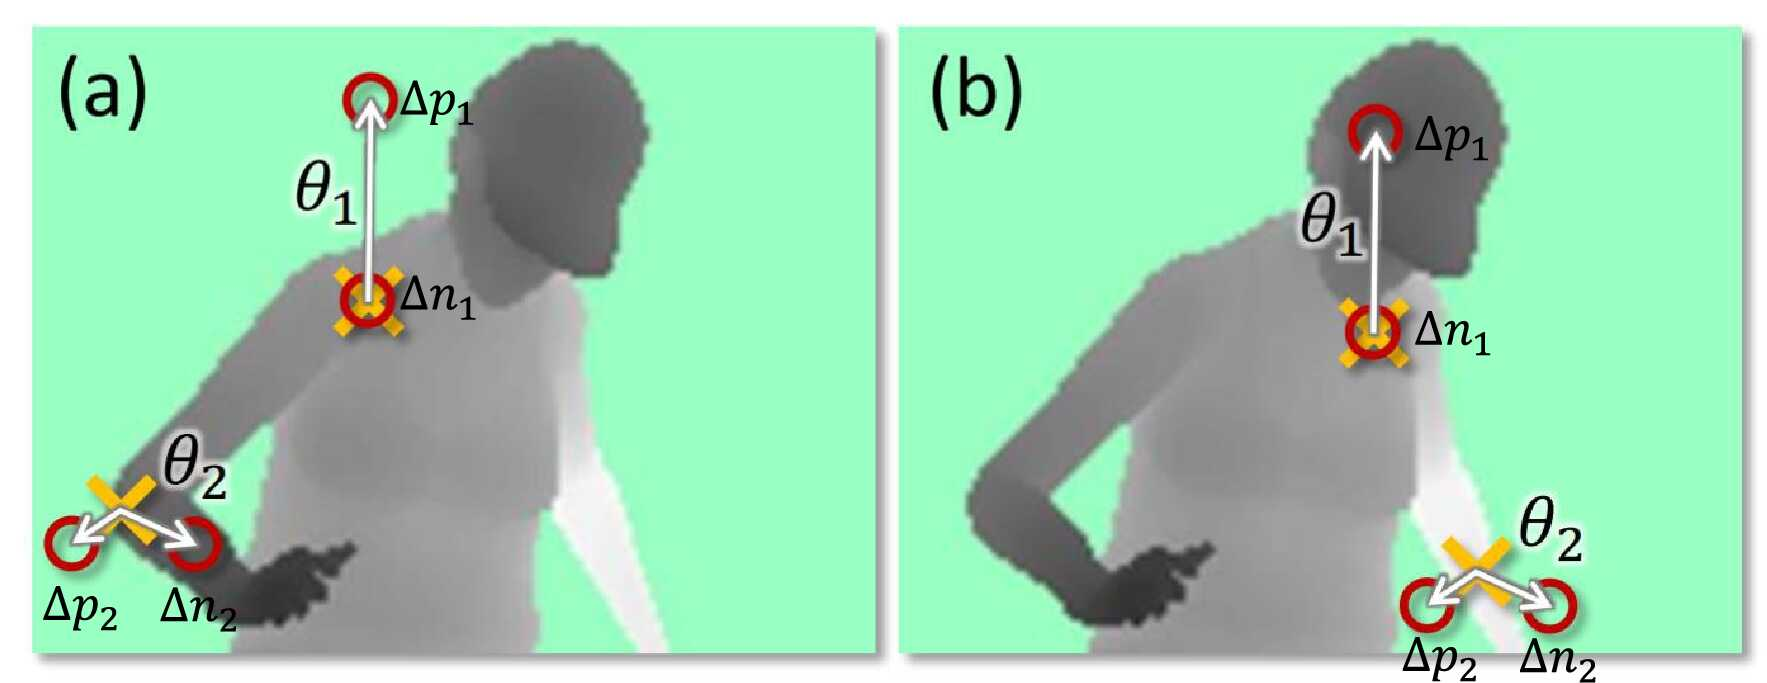
\includegraphics[width=0.6\linewidth]{./img/_depth_comparison_features.jpg}
            \caption{Examples of feature computation}
        \end{figure}

        \begin{description}
            \item[Depth-invariant offsets]
                The denominator ($D[x]$) applied to the offsets allows obtaining depth-invariant offsets.

                Consider two objects at different depths. The focal length of the camera is $f$ and the world offset we want to apply is $o_w$. By changing depth $d$, the offset in the image plane $o_{di}$ changes due to the perspective projection rules. Therefore, to obtain the offset in the image plane, we have that:
                \[ o_{di} : f = o_w : d \,\Rightarrow\, o_{di} = \frac{o_w f}{d} = \frac{\Delta p}{d} \]

                \begin{figure}[H]
                    \centering
                    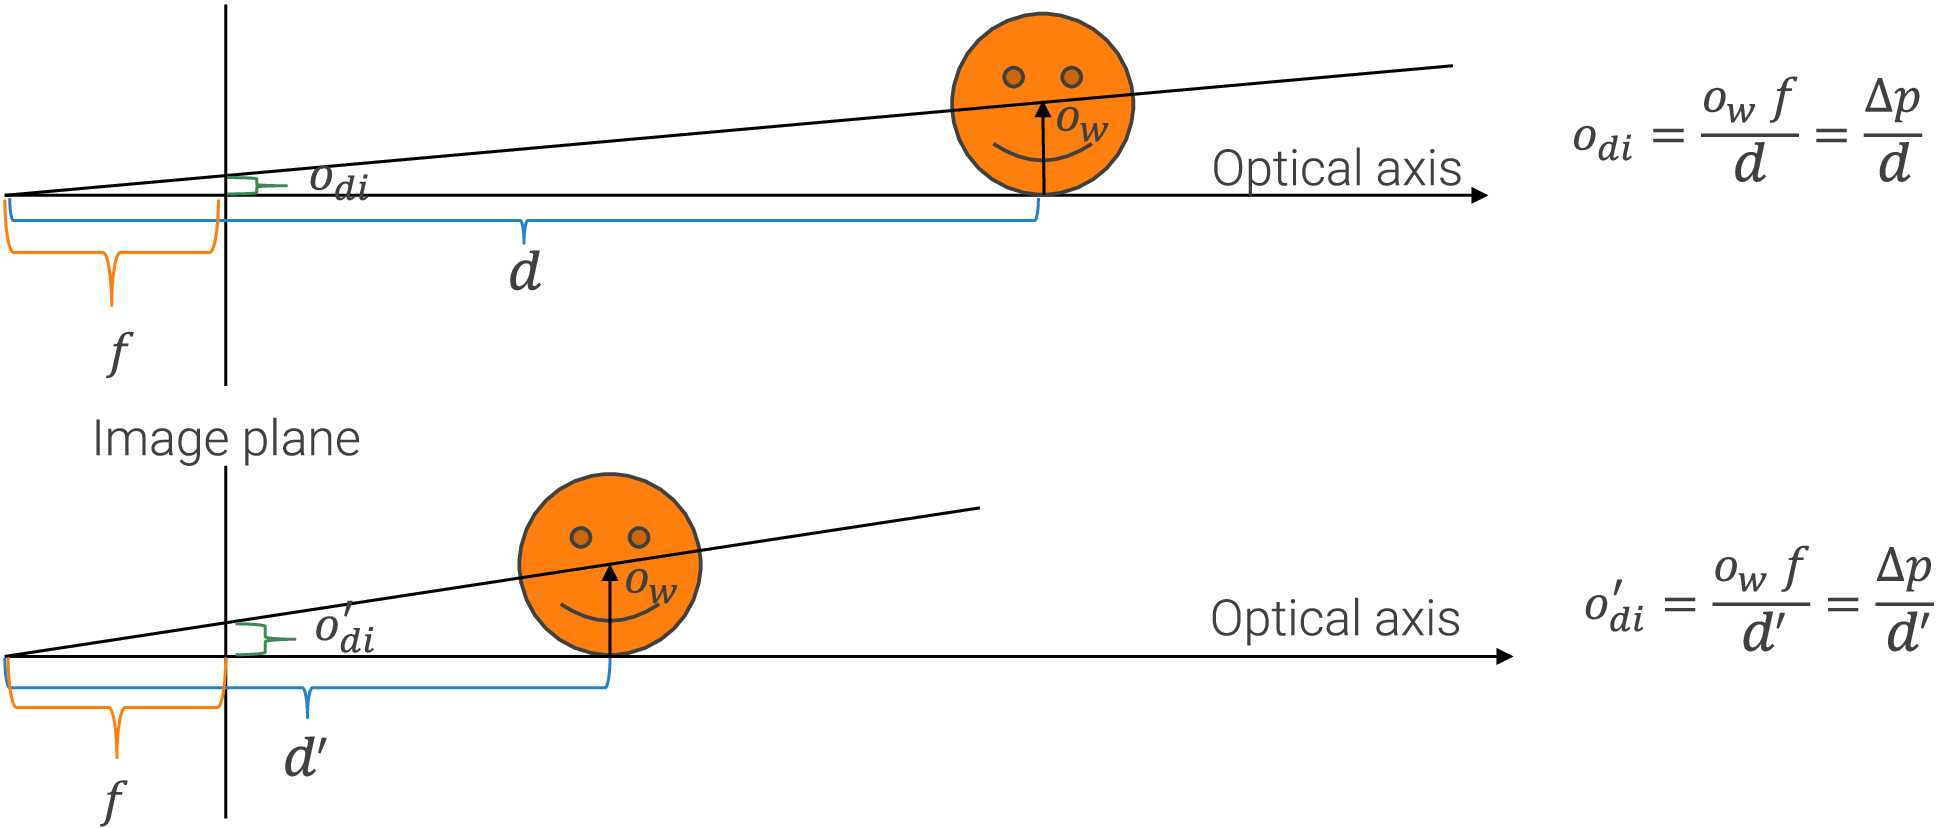
\includegraphics[width=0.6\linewidth]{./img/_depth_invariant_offset.jpg}
                \end{figure}
        \end{description}

    \item[Decision tree] \marginnote{Decision tree}
        Depth comparison features are used to train decision trees.

        \begin{remark}
            Decision trees are unstable robust classifiers. They are able to achieve good performance but significantly change in structure if the training data is slightly perturbed (i.e., high variance).
        \end{remark}

        \begin{description}
            \item[Random forest] \marginnote{Random forest}
                Ensemble of $N$ decision trees that aims to reduce variance by averaging their predictions.

                \begin{remark}
                    For a random forest to be effective, its decision trees should be uncorrelated so that when averaging, the average of their errors tend to $0$.
                \end{remark}

                \begin{description}
                    \item[Bootstrap aggregating (bagging)] \marginnote{Bootstrap aggregating (bagging)}
                        Train each decision tree using a replica of the training set obtained by sampling with replacement.

                        \begin{figure}[H]
                            \raggedleft
                            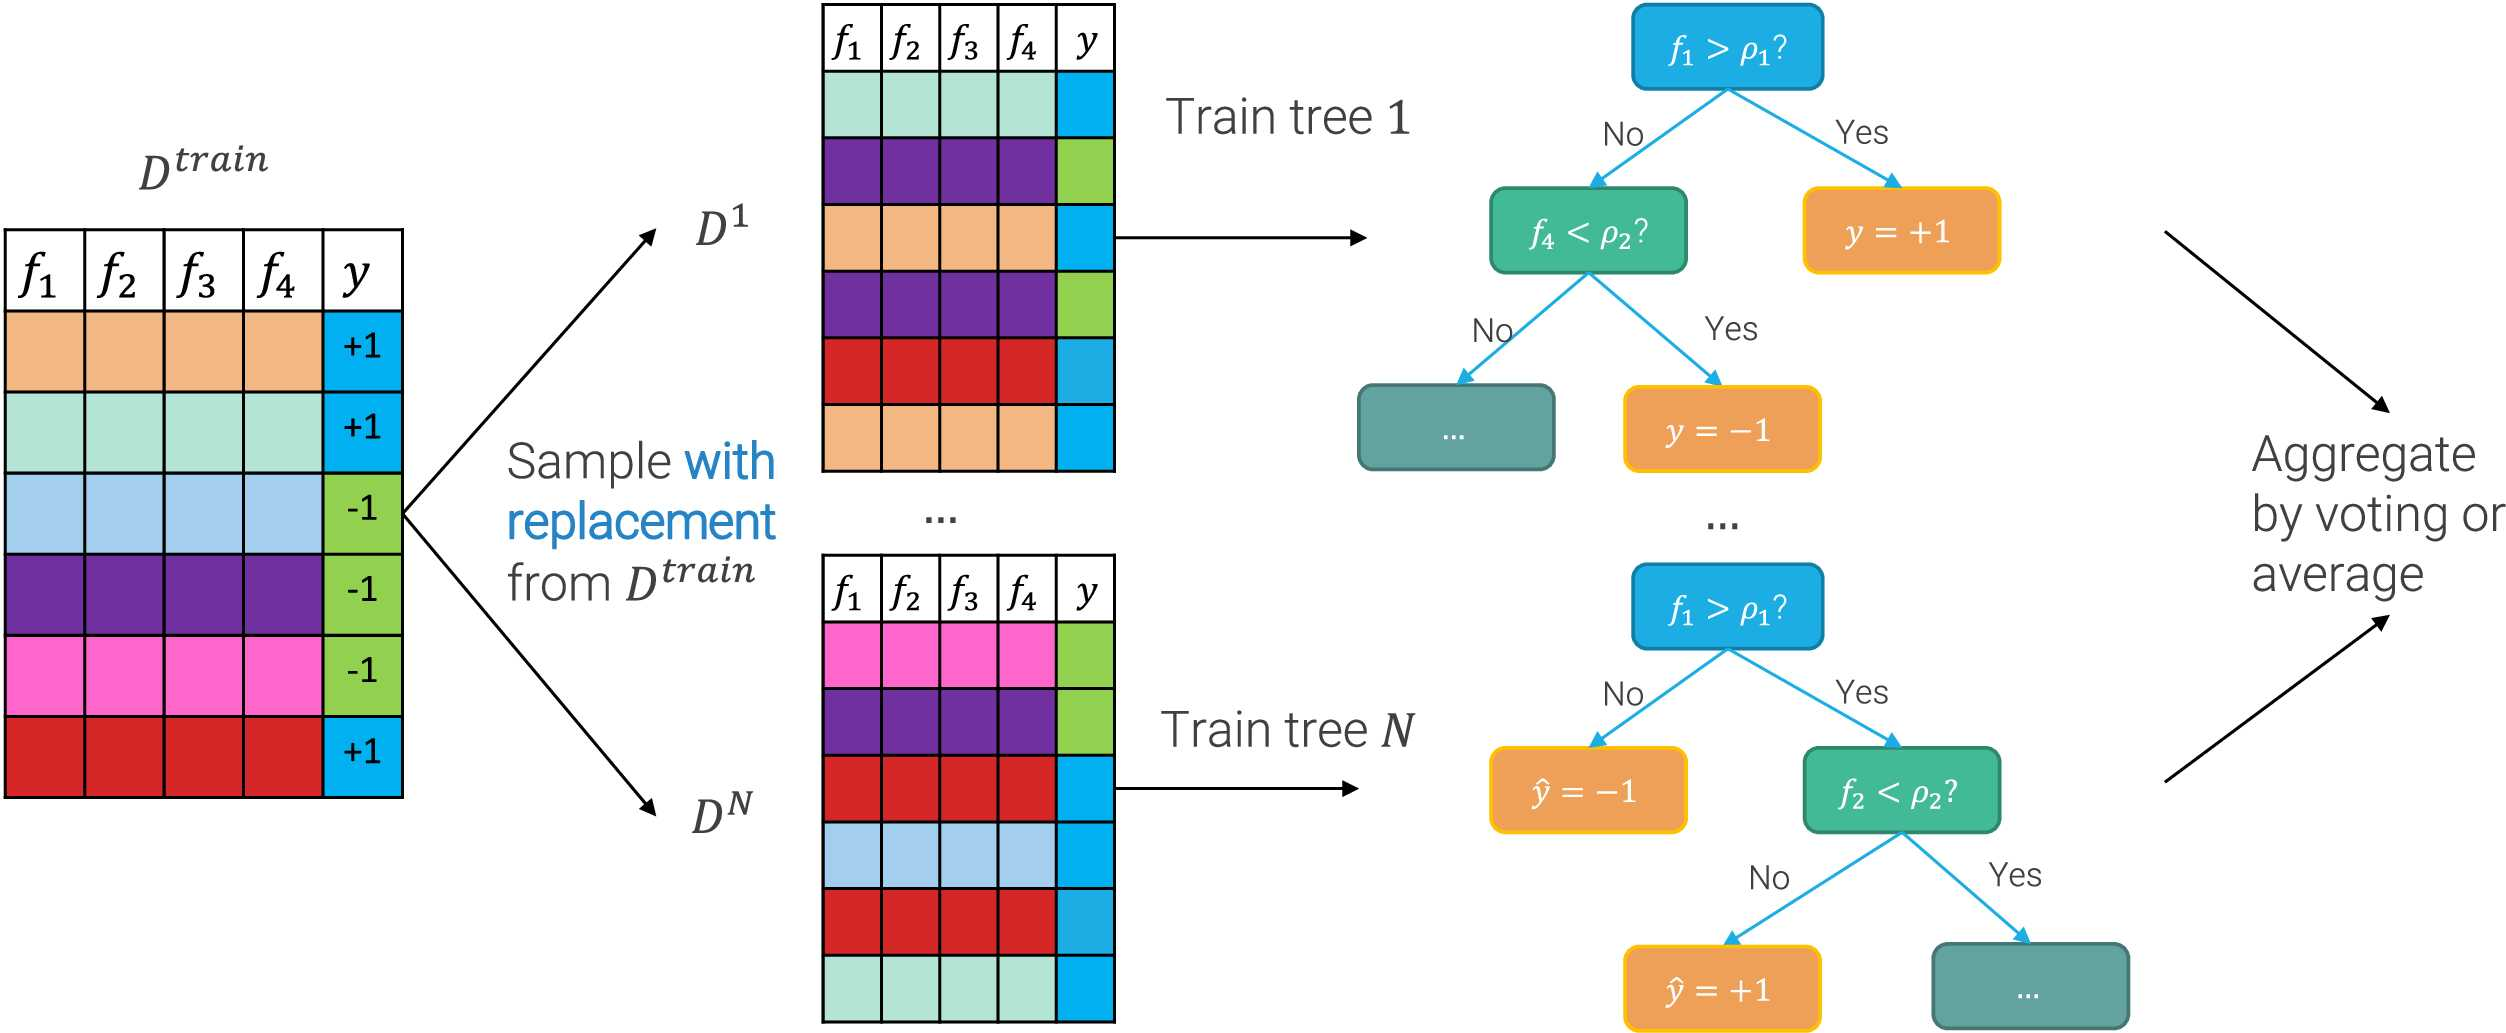
\includegraphics[width=0.7\linewidth]{./img/_random_forest_bagging.jpg}
                        \end{figure}

                    \item[Random splitting] \marginnote{Random splitting}
                        Even though bagging reduces variance, if there is a subset of particularly predictive features, the resulting trees will be correlated. 

                        To avoid this, in a random forest, tree splitting is done on a different random subset of features each time.

                        \begin{figure}[H]
                            \raggedleft
                            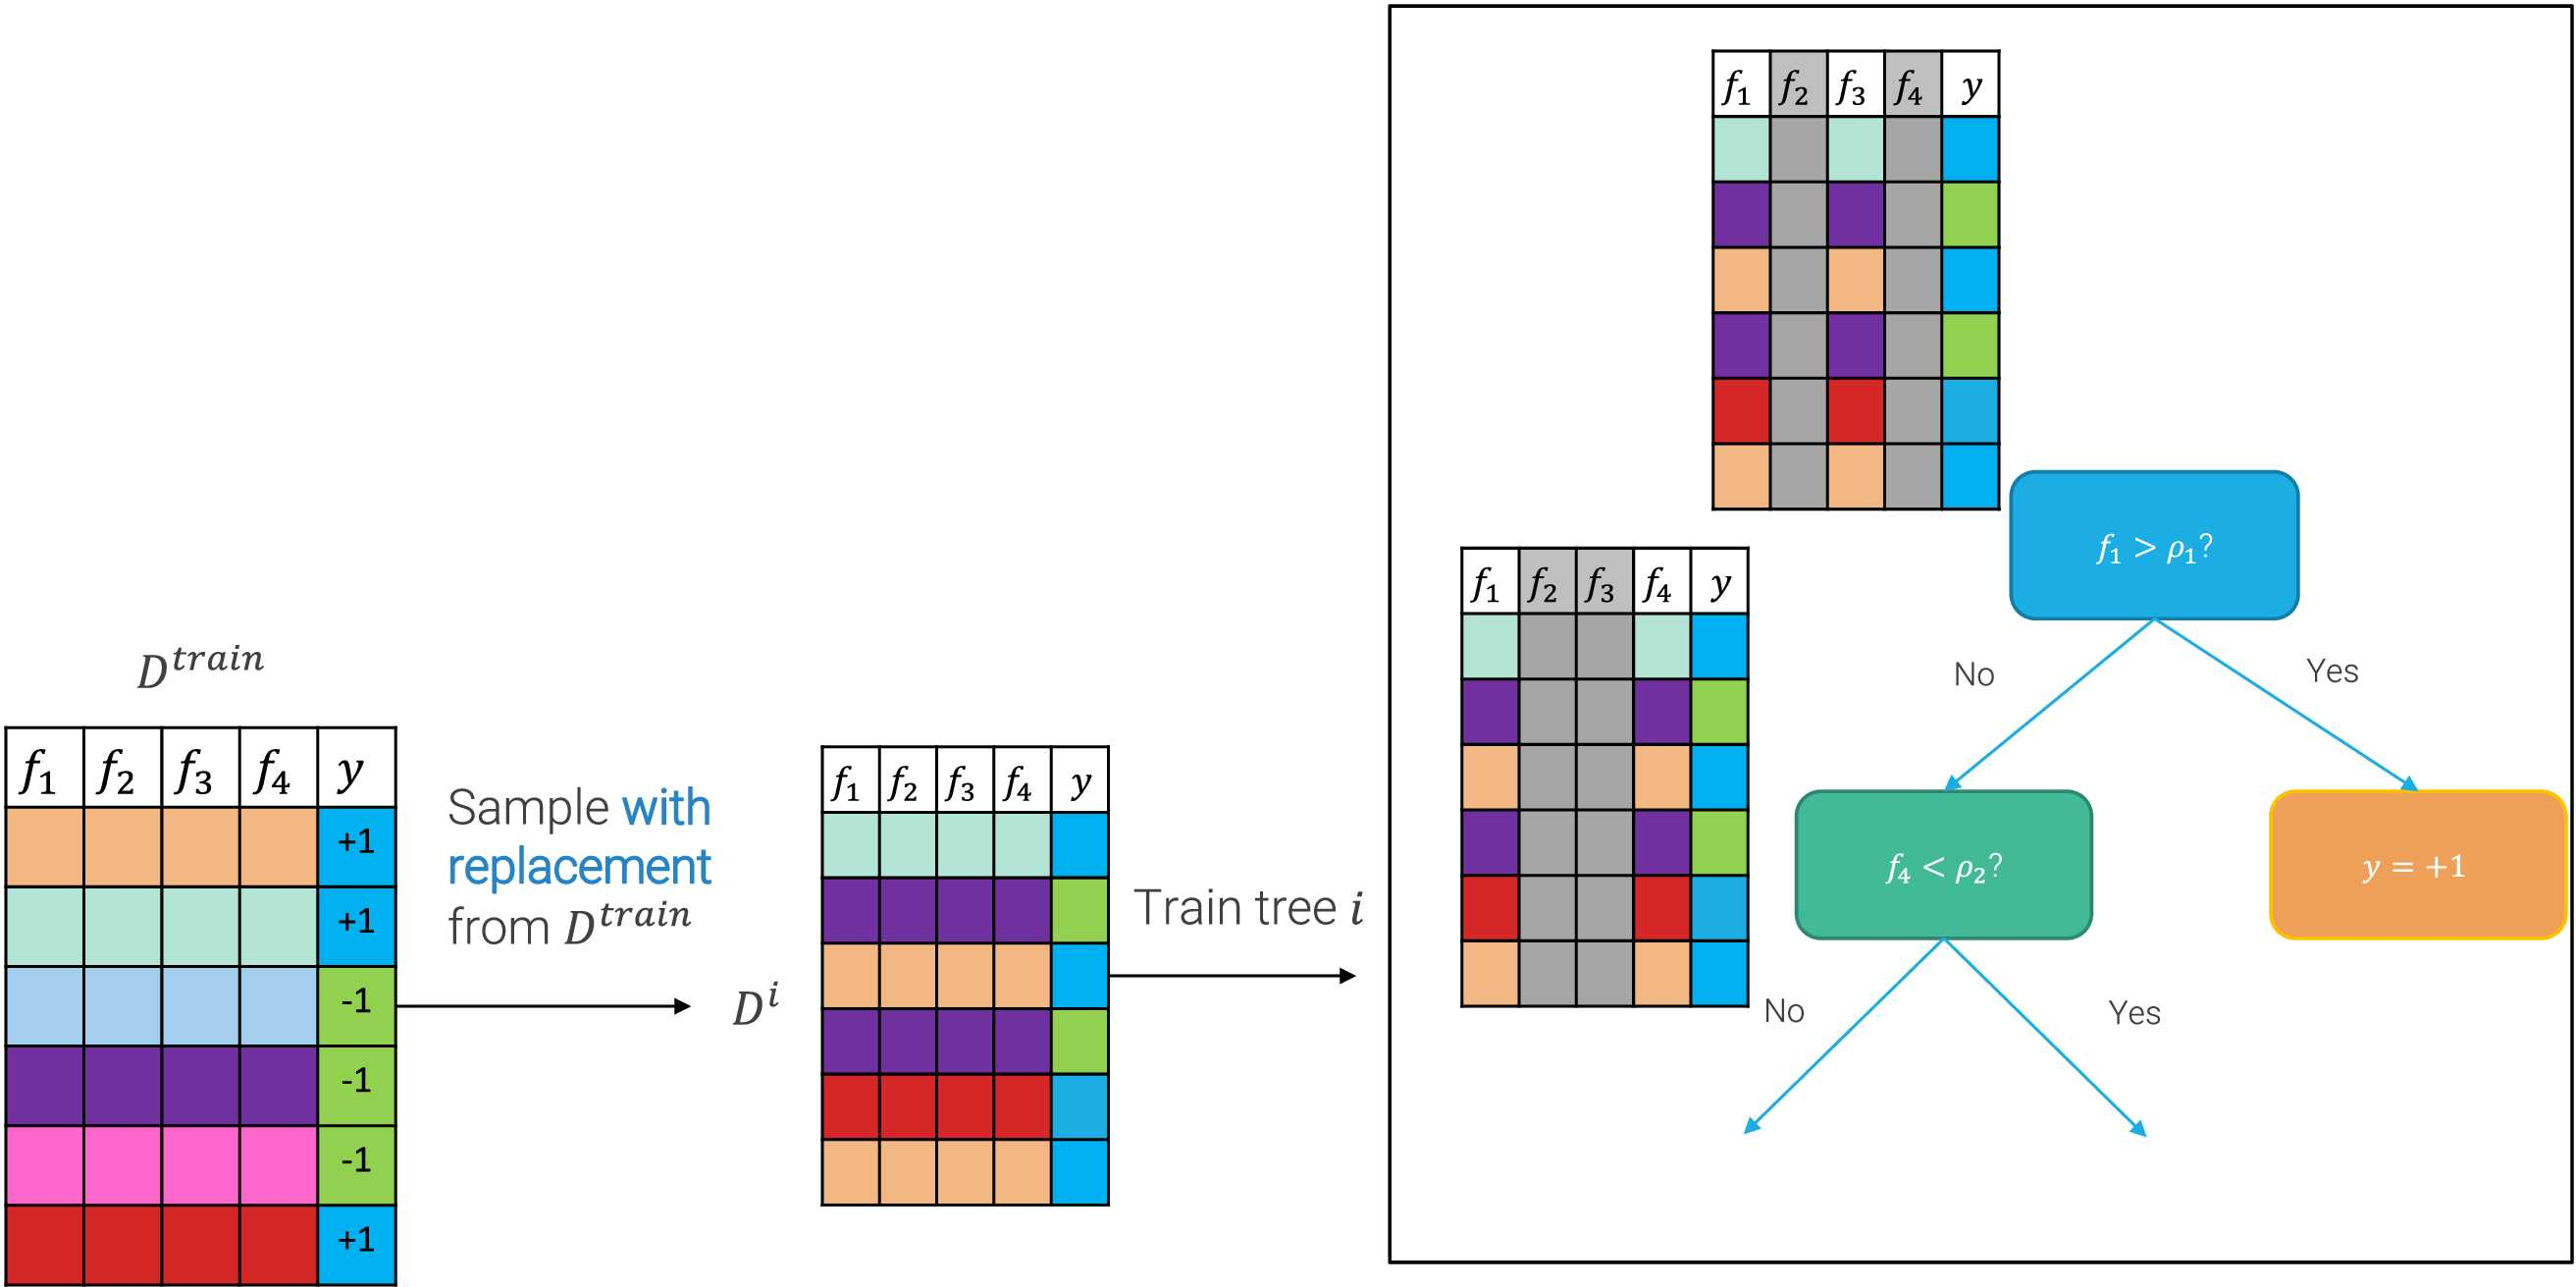
\includegraphics[width=0.7\linewidth]{./img/_random_forest_random_splitting.jpg}
                        \end{figure}
                \end{description}

                \begin{remark}
                    Random forests are:
                    \begin{itemize}
                        \item Fast and parallelizable at both training and inference.
                        \item Robust to hyperparameters change.
                        \item Interpretable.
                    \end{itemize}
                \end{remark}
        \end{description}
\end{description}


\subsection{R-CNN}

\begin{description}
    \item[R-CNN for segmentation] \marginnote{R-CNN for segmentation}
        Slide a window across each pixel of the input image. Each slice is passed through an R-CNN to determine the class of the pixel at the center of the window.

        The loss for an example $i$ is the sum of the cross-entropy losses at each pixel $(u, v)$:
        \[ \mathcal{L}^{(i)} = \sum_{(u, v)} \mathcal{L}_\text{CE}\left( \texttt{softmax}(\texttt{scores}_{(u, v)}), \mathbbm{1}\left( c_{(u, v)}^{(i)} \right) \right) \]

        \begin{figure}[H]
            \centering
            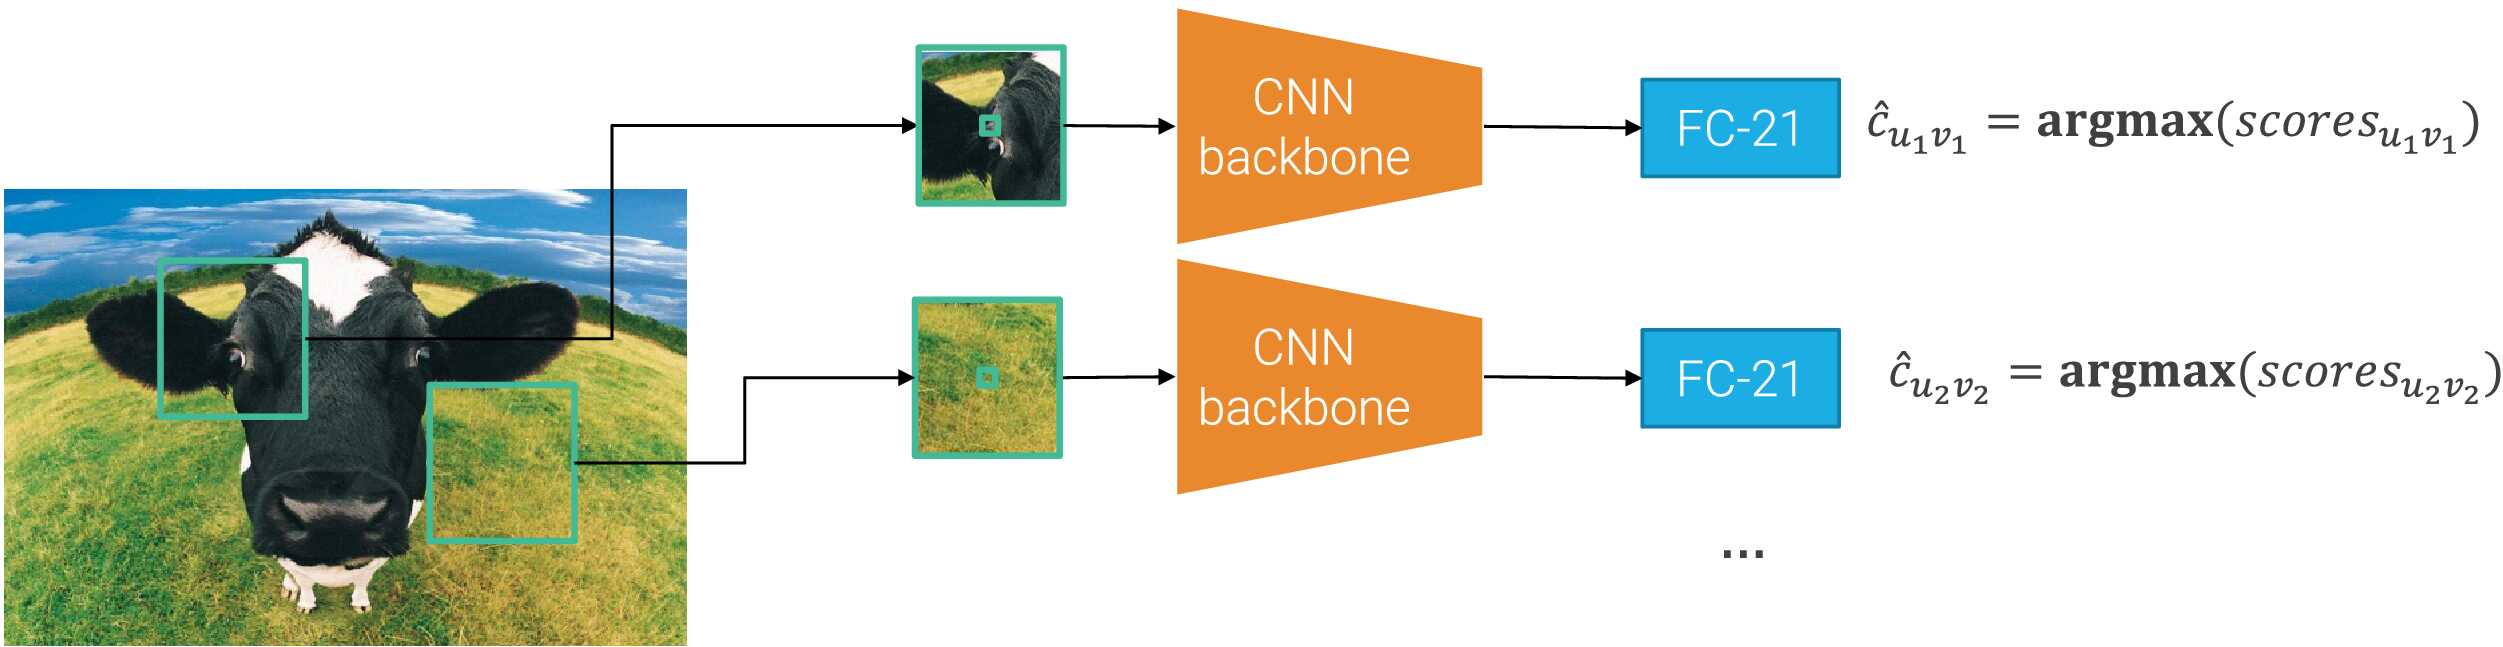
\includegraphics[width=0.9\linewidth]{./img/_segmentation_rcnn.jpg}
            \caption{R-CNN for segmentation with $20$ ($+1$) classes}
        \end{figure}
\end{description}


\subsection{Fully convolutional network}

\begin{description}
    \item[Standard up-sampling] \marginnote{Standard up-sampling}
        Non-learned operator to increase the spatial dimension of the input image. Possible approaches are:
        \begin{descriptionlist}
            \item[Nearest neighbor]
                Fill the new pixels with the value of the nearest one.
            \item[Bilinear interpolation]
                Fill the new pixels by interpolating the nearest ones.
        \end{descriptionlist}

    \item[Fully convolutional network (FCN)] \marginnote{Fully convolutional network (FCN)}
        Pass the whole input image into a CNN and use the activation to determine the class of each pixel. The flow is the following:
        \begin{descriptionlist}
            \item[Backbone] Pass the input image through a CNN.
            \item[Scoring layer] Apply a $1 \times 1$ convolution on the output activation to obtain the correct number of channels (one per class).
            \item[Up-sampling] Apply an up-sampling operator to restore the input spatial dimension.
        \end{descriptionlist}

        \begin{remark}
            Without learned non-linear up-sampling operators, the output mask is dependent on the total stride of the CNN. Therefore, a coarse final activation will result in a coarse segmentation mask.
        \end{remark}

        \begin{description}
            \item[Pyramid of FCNs] \marginnote{Pyramid of FCNs}
                Stack of FCNs with skips (i.e., merges) to up-sample multiple activations at different resolutions.
                \begin{descriptionlist}
                    \item[FCN-32S] 
                        FCN that applies the backbone CNN up until the last layer $L$ obtaining a total stride of $32$. This results in a very coarse mask.

                        \begin{figure}[H]
                            \raggedleft
                            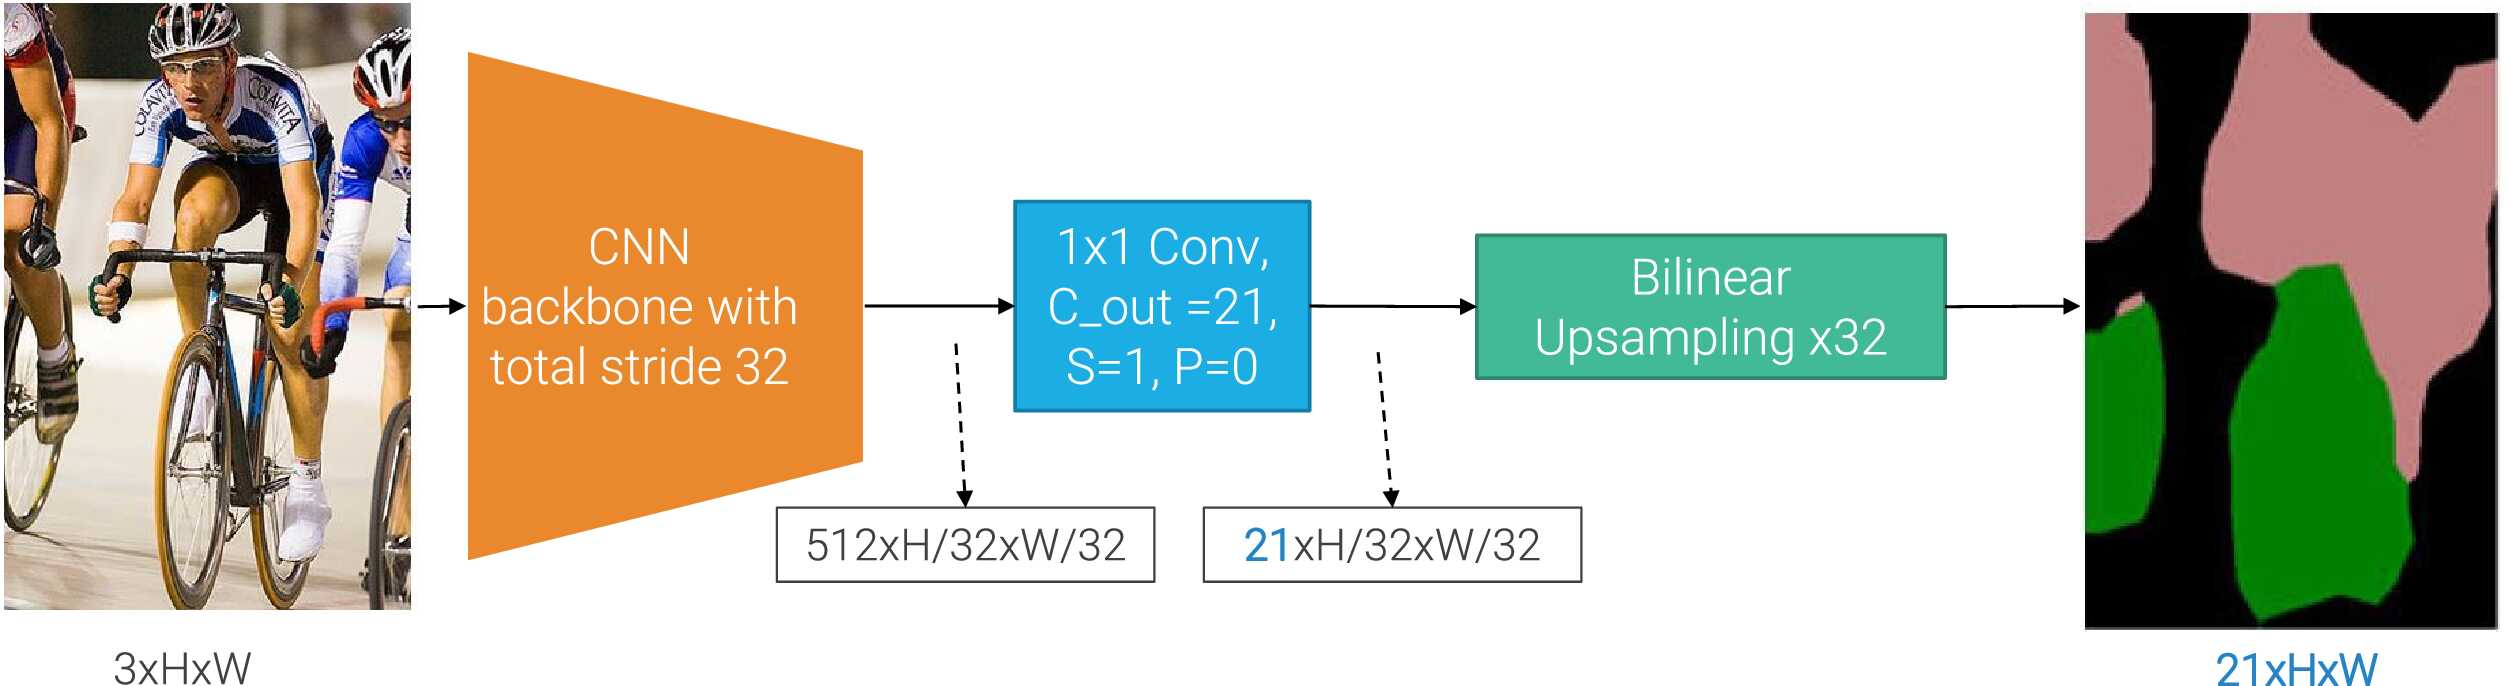
\includegraphics[width=0.85\linewidth]{./img/_fcn_32.jpg}
                        \end{figure}

                    \item[FCN-16S] 
                        FCN that applies the backbone CNN up until the layer $L-1$ and then branches into two paths:
                        \begin{itemize}
                            \item A branch continues into the $L$-th layer as in FCN-32S. Up-sampling is done to match the spatial dimension of the other branch so that it can be used as a skip.
                            \item A branch passes through a scoring layer and is summed to the output of the other branch before up-sampling to the image spatial dimension.
                        \end{itemize}

                        \begin{figure}[H]
                            \raggedleft
                            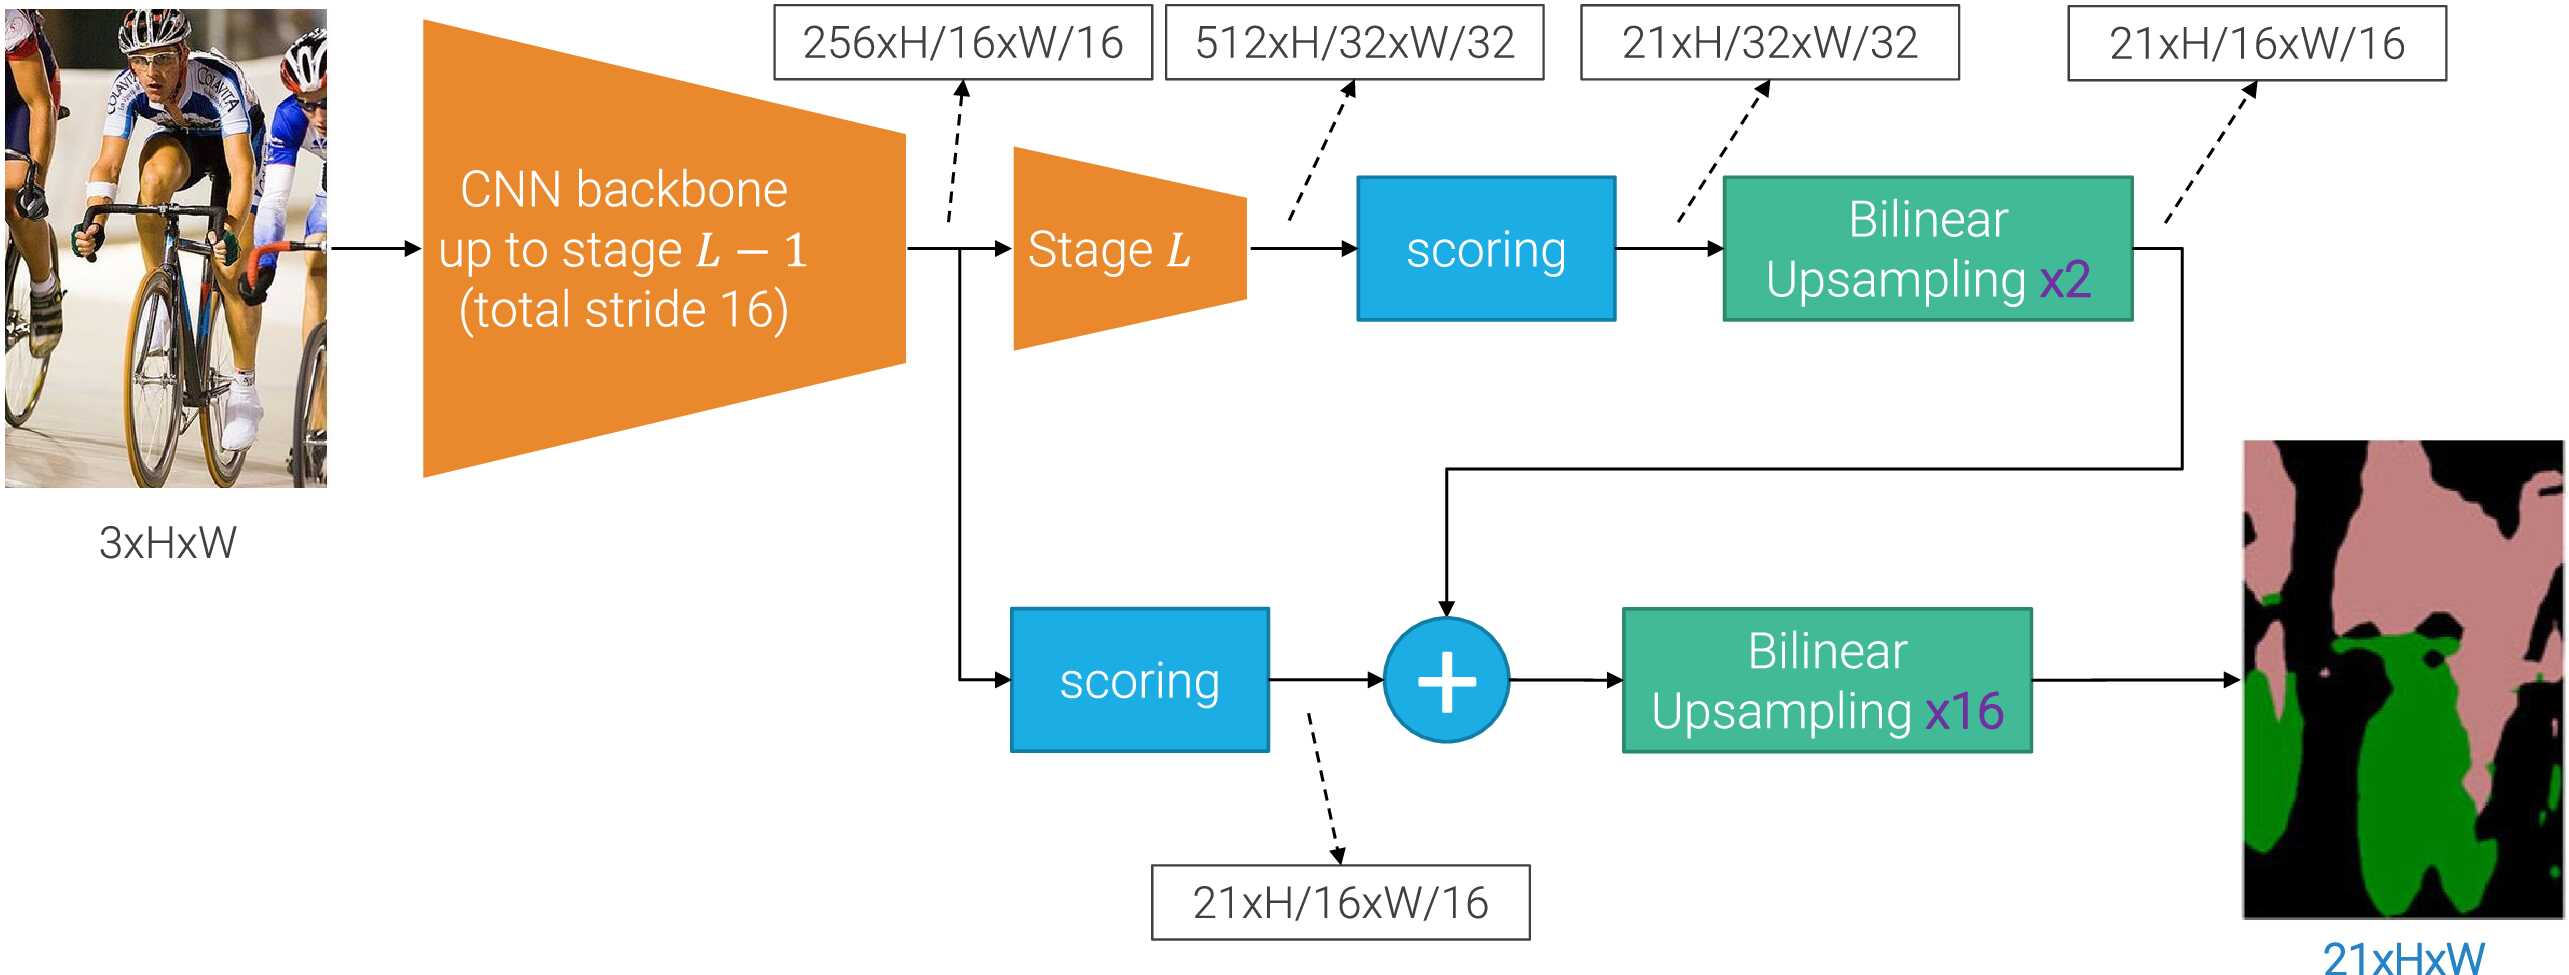
\includegraphics[width=0.85\linewidth]{./img/_fcn_16.jpg}
                        \end{figure}

                    \item[FCN-8S] 
                        As FCN-16S where the skip comes from FCN-16S.

                        \begin{figure}[H]
                            \raggedleft
                            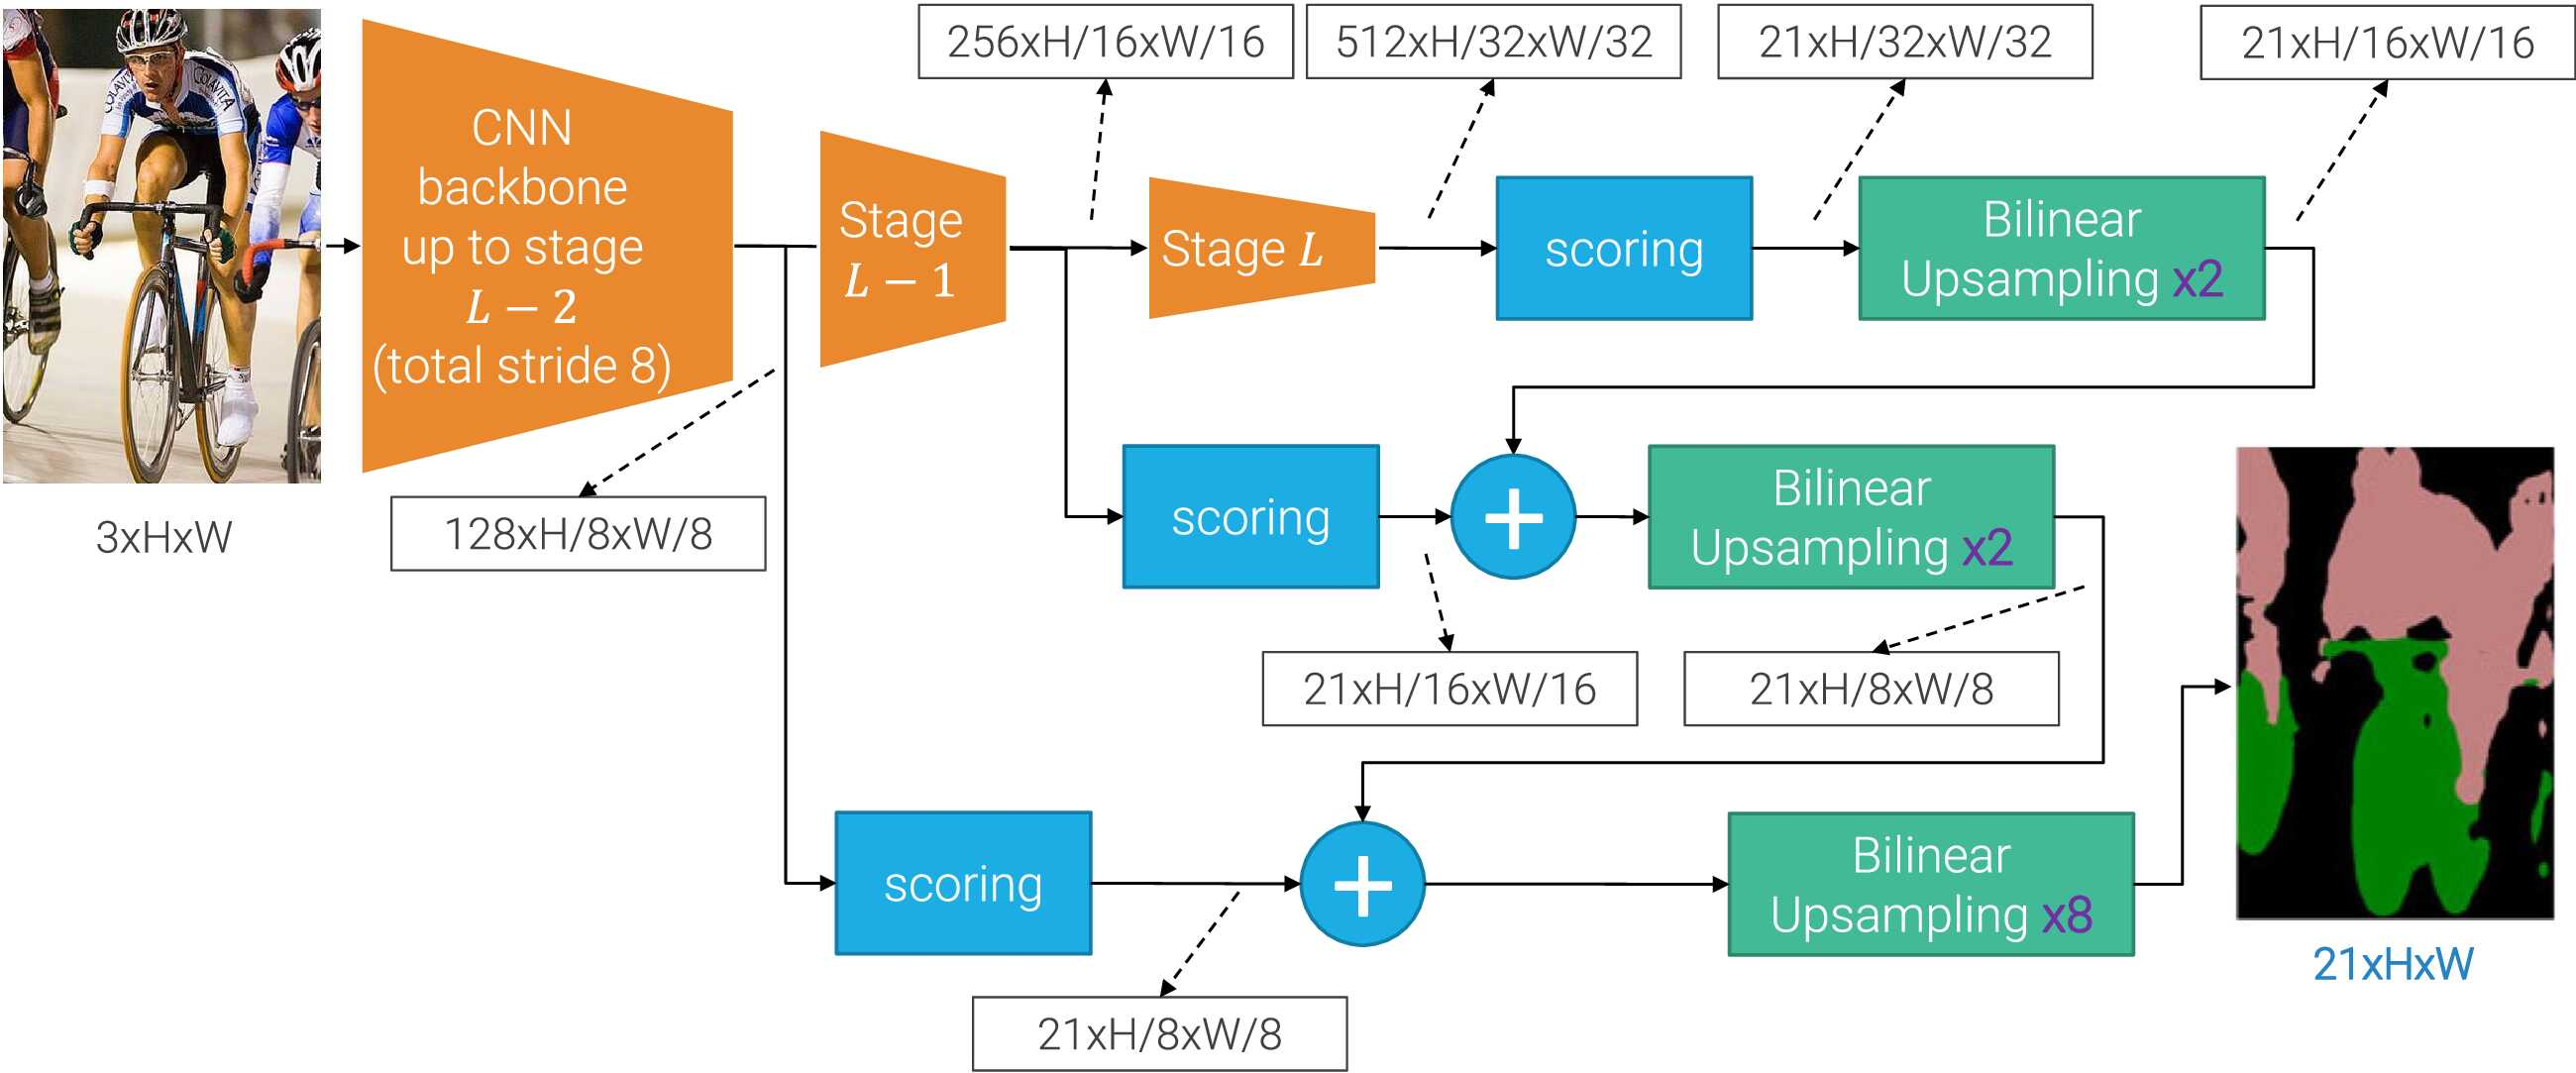
\includegraphics[width=0.85\linewidth]{./img/_fcn_8.jpg}
                        \end{figure}
                \end{descriptionlist}

                \begin{remark}
                    Ablation study found out that:
                    \begin{itemize}
                        \item Results do not show significant improvements after stride $8$ (i.e., the initial stages of the backbone CNN are less relevant for the segmentation task).
                        \item Fine-tuning the backbone is important.
                        \item There is no significant difference in training end-to-end (i.e., directly FCN-8S) and coarse-to-fine (i.e., progressively train starting from FCN-32S up to FCN-8S)
                        \item Skips between resolutions to merge them are important.
                    \end{itemize}
                \end{remark}
        \end{description}
\end{description}


\subsection{U-Net}

\begin{description}
    \item[Transposed convolution] \marginnote{Transposed convolution}
        Operator to invert the spatial down-sampling of a convolution.

        Given a convolution with convolutional matrix $K$, a transposed convolution is obtained by applying $K^T$ to the image.

        In practice, a transposed convolution can be obtained by sliding the kernel on the output activation (instead of input). The values at the output activation correspond to the product between the input pixels and the kernel. If multiple kernels overlap at the same output pixel, its value is obtained as the sum of all the values that end up in that position.

        \begin{example}
            Consider images with $1$ channel. Given a $3 \times 3$ input image and a $3 \times 3$ transposed convolution kernel with stride $2$, the output activation has spatial dimension $5 \times 5$ and is obtained as follows:
            \begin{figure}[H]
                \centering
                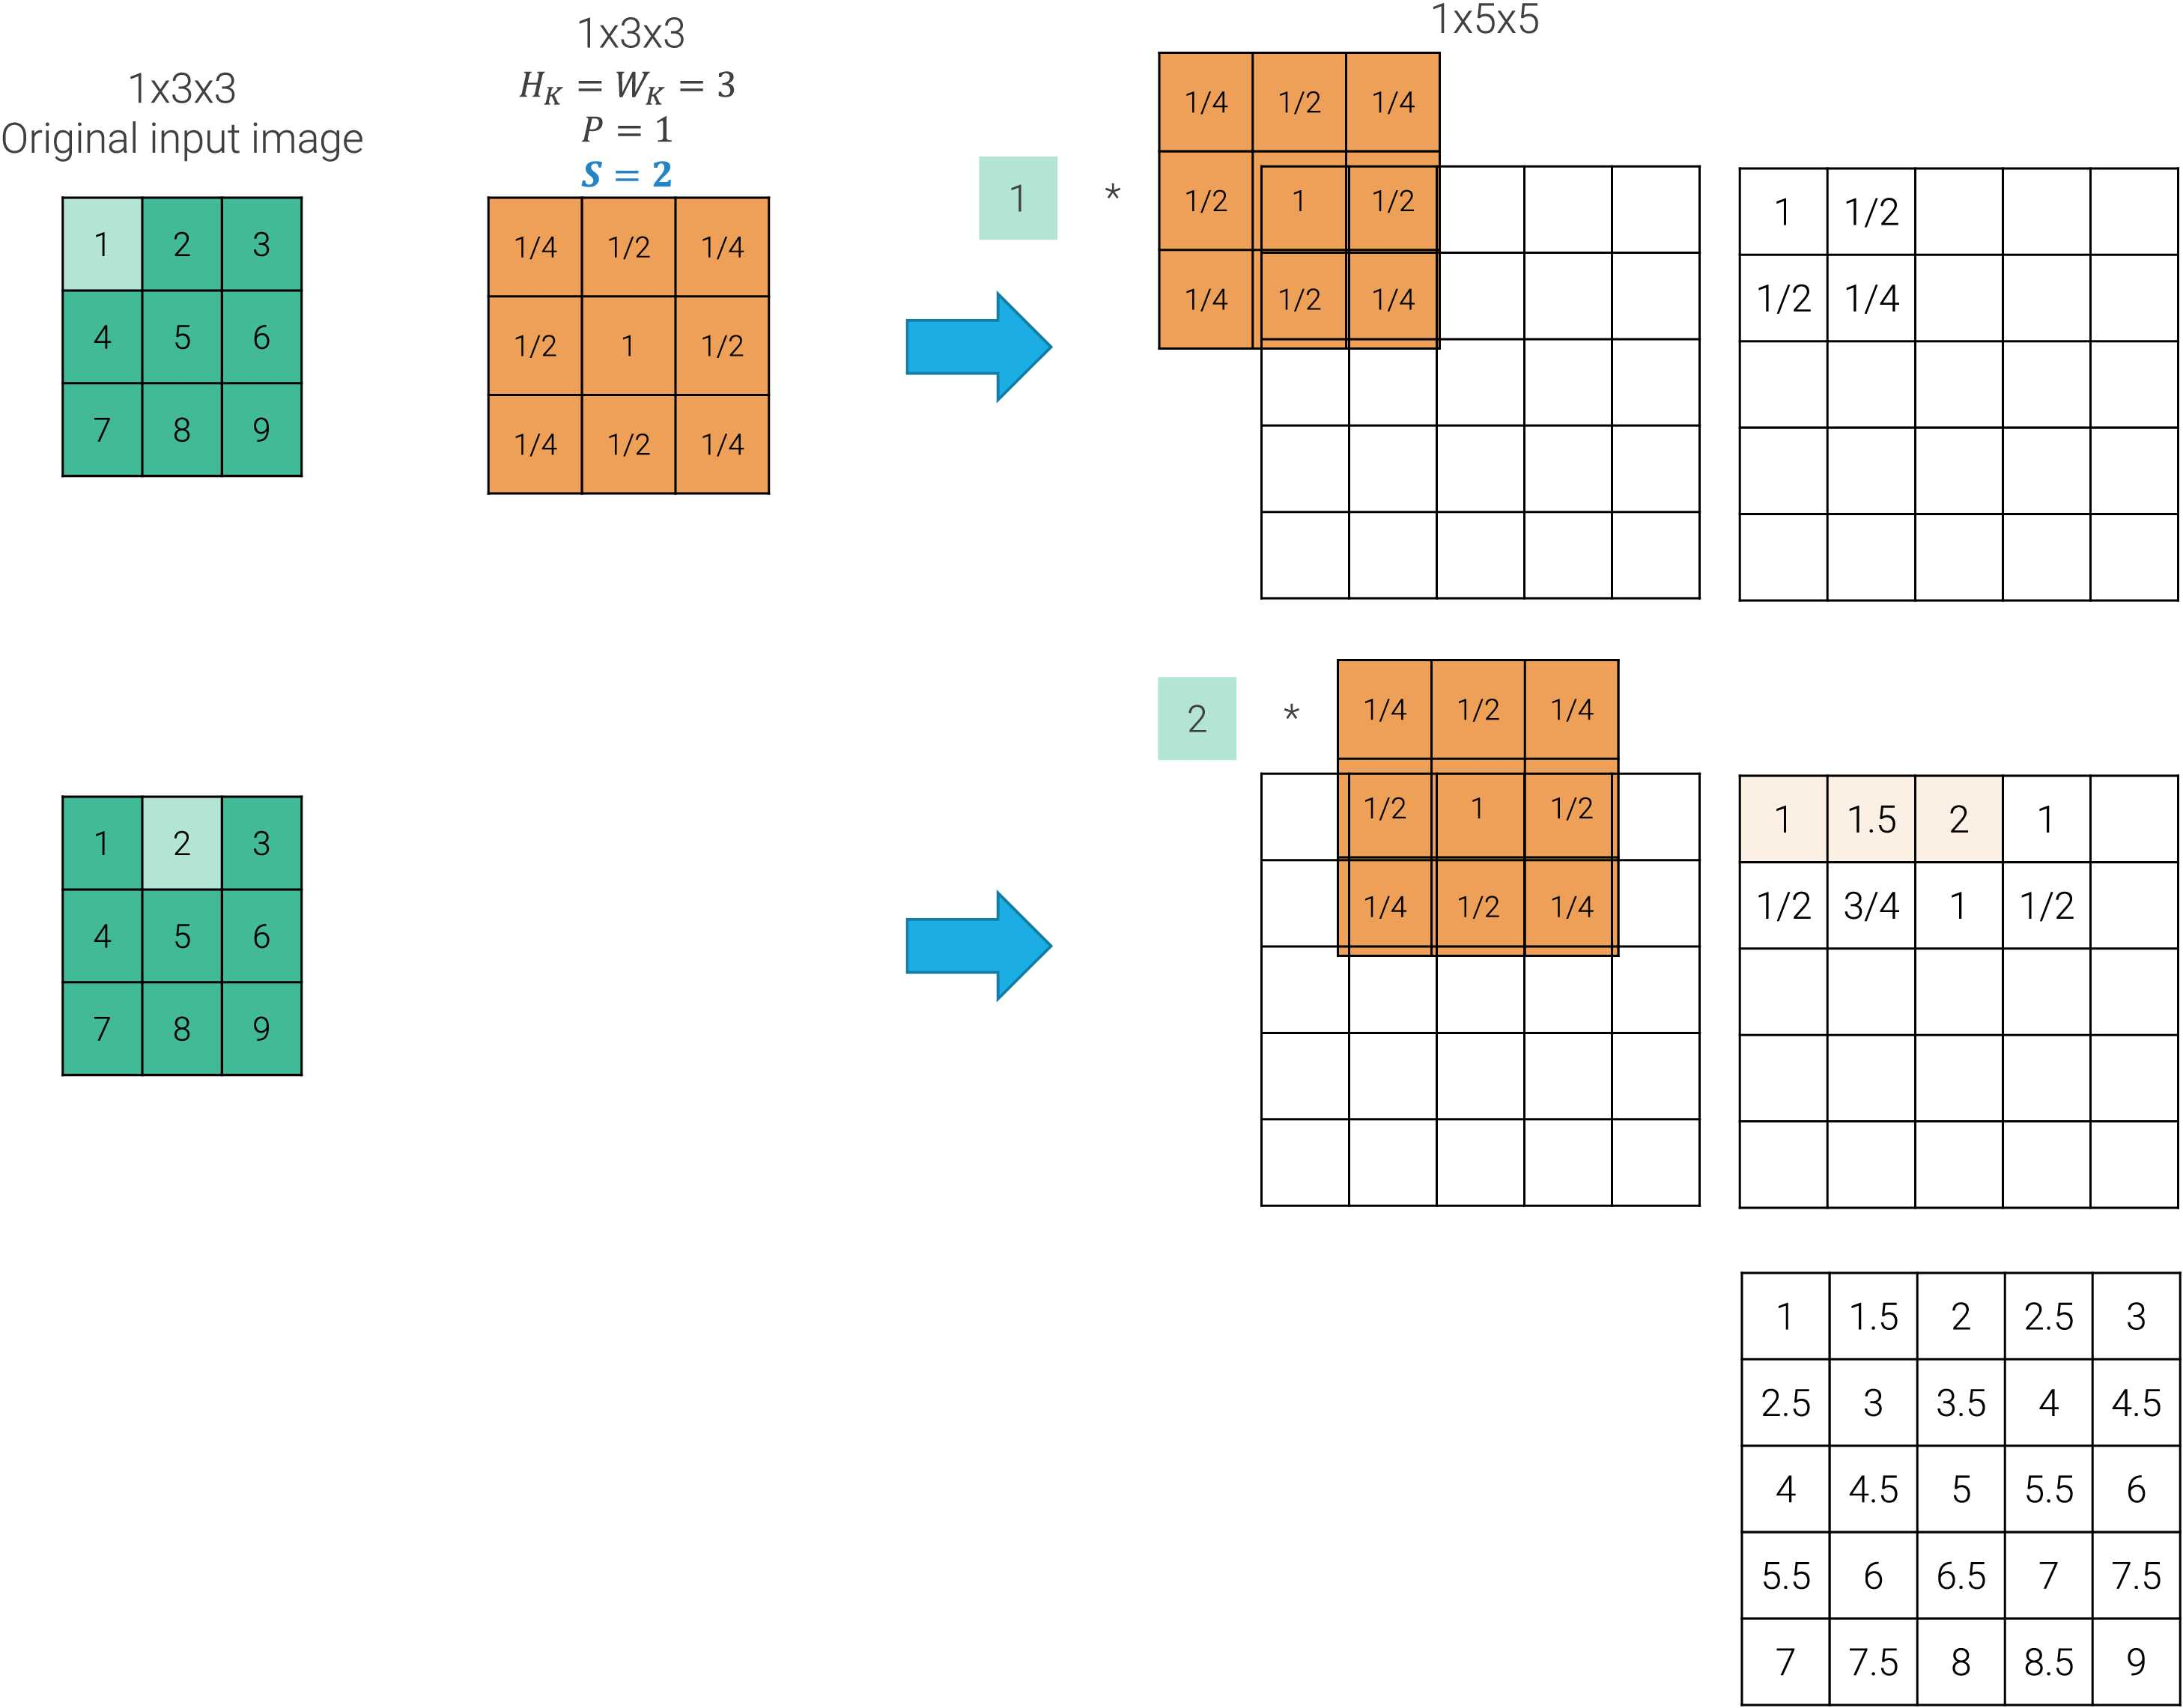
\includegraphics[width=0.9\linewidth]{./img/_transposed_convolution.jpg}
            \end{figure}
        \end{example}

        \begin{remark}
            A transposed convolution is usually initialized as a bilinear interpolator. For instance, a $3 \times 3$ kernel is initialized as:
            \[ 
                \begin{bmatrix}
                    \frac{1}{4} & \frac{1}{2} & \frac{1}{4} \\
                    \frac{1}{2} & 1 & \frac{1}{2} \\
                    \frac{1}{4} & \frac{1}{2} & \frac{1}{4} \\
                \end{bmatrix}
            \]
        \end{remark}

        \begin{remark}
            Transposed convolutions can be seen as convolutions with a fractional stride.
        \end{remark}

        \begin{remark}
            Transposed convolutions are also called deconvolutions (this is technically wrong as deconvolutions are the full inverse of convolutions), up-convolutions, fractionally/backward strided convolutions.
        \end{remark}

        \begin{remark}
            In generative tasks, transposed convolutions generate checkerboard artifacts. Darker pixels are due to the fact that they result from the summation of multiple kernel applications.
        \end{remark}

    \item[U-Net] \marginnote{U-Net}
        Encoder-decoder architecture for segmentation:
        \begin{descriptionlist}
            \item[Encoder] Backbone CNN that down-samples the input image.
            \item[Decoder] Symmetric structure to the encoder that up-samples the activation using transposed convolutions and further refines them with normal $3 \times 3$ convolutions.
        \end{descriptionlist}
        Each level of the encoder is connected to its corresponding level in the decoder through a skip connection that concatenates the activations.

        The scoring layer is only applied at the end to adjust the number of channels.

        \begin{figure}[H]
            \centering
            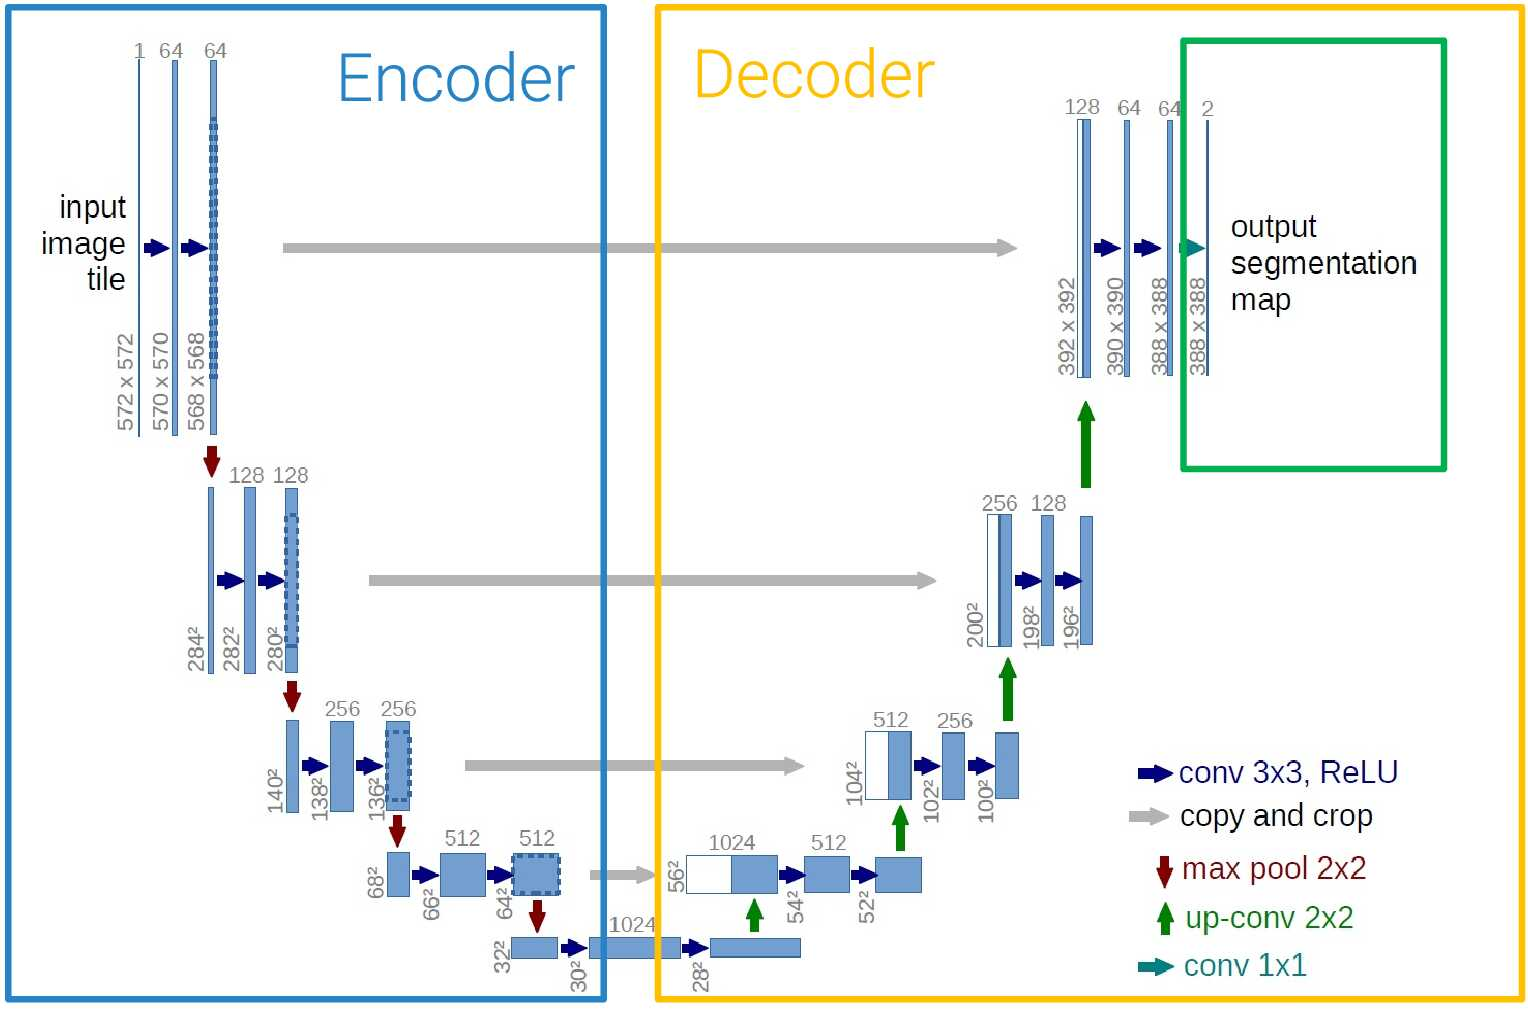
\includegraphics[width=0.6\linewidth]{./img/_unet.jpg}
            \caption{
                \parbox[t]{0.7\linewidth}{
                    U-Net structure. Note that in the original paper, convolutions have padding \texttt{valid} and the input is provided from a sliding window. Modern implementations have padding \texttt{same} and same input and output spatial dimension.
                }
            }
        \end{figure}

        \begin{remark}
            Intuitively, the two components of a U-Net do the following:
            \begin{descriptionlist}
                \item[Encoder] Determine what is in the image.
                \item[Decoder] Determine where the objects are.
            \end{descriptionlist}
        \end{remark}
\end{description}


\subsection{Dilated CNN}

\begin{remark}
    The standard classification backbone approach has some shortcomings:
    \begin{itemize}
        \item Predictions made using the activation at higher layers are semantically rich but spatially coarse.
        \item Predictions made using the activation at lower layers are semantically poorer but have a higher spatial resolution.
    \end{itemize}
\end{remark}

\begin{description}
    \item[Dilated/atrous convolution] \marginnote{Dilated/atrous convolution}
        Given a dilation rate $r$, a dilated convolution is equivalent to applying a kernel with an $r-1$ gap between weights.

        Formally, a dilated convolution with kernel $K$ and dilation rate $r$ applied on an image $I$ is computed as follows:
        \[
            [K * I](j, i) = \sum_{n=1}^{C} \sum_{m} \sum_{l} K_n(m, l) I_n(j - r \cdot m, i - r \cdot l) + b
        \]

        \begin{figure}[H]
            \centering
            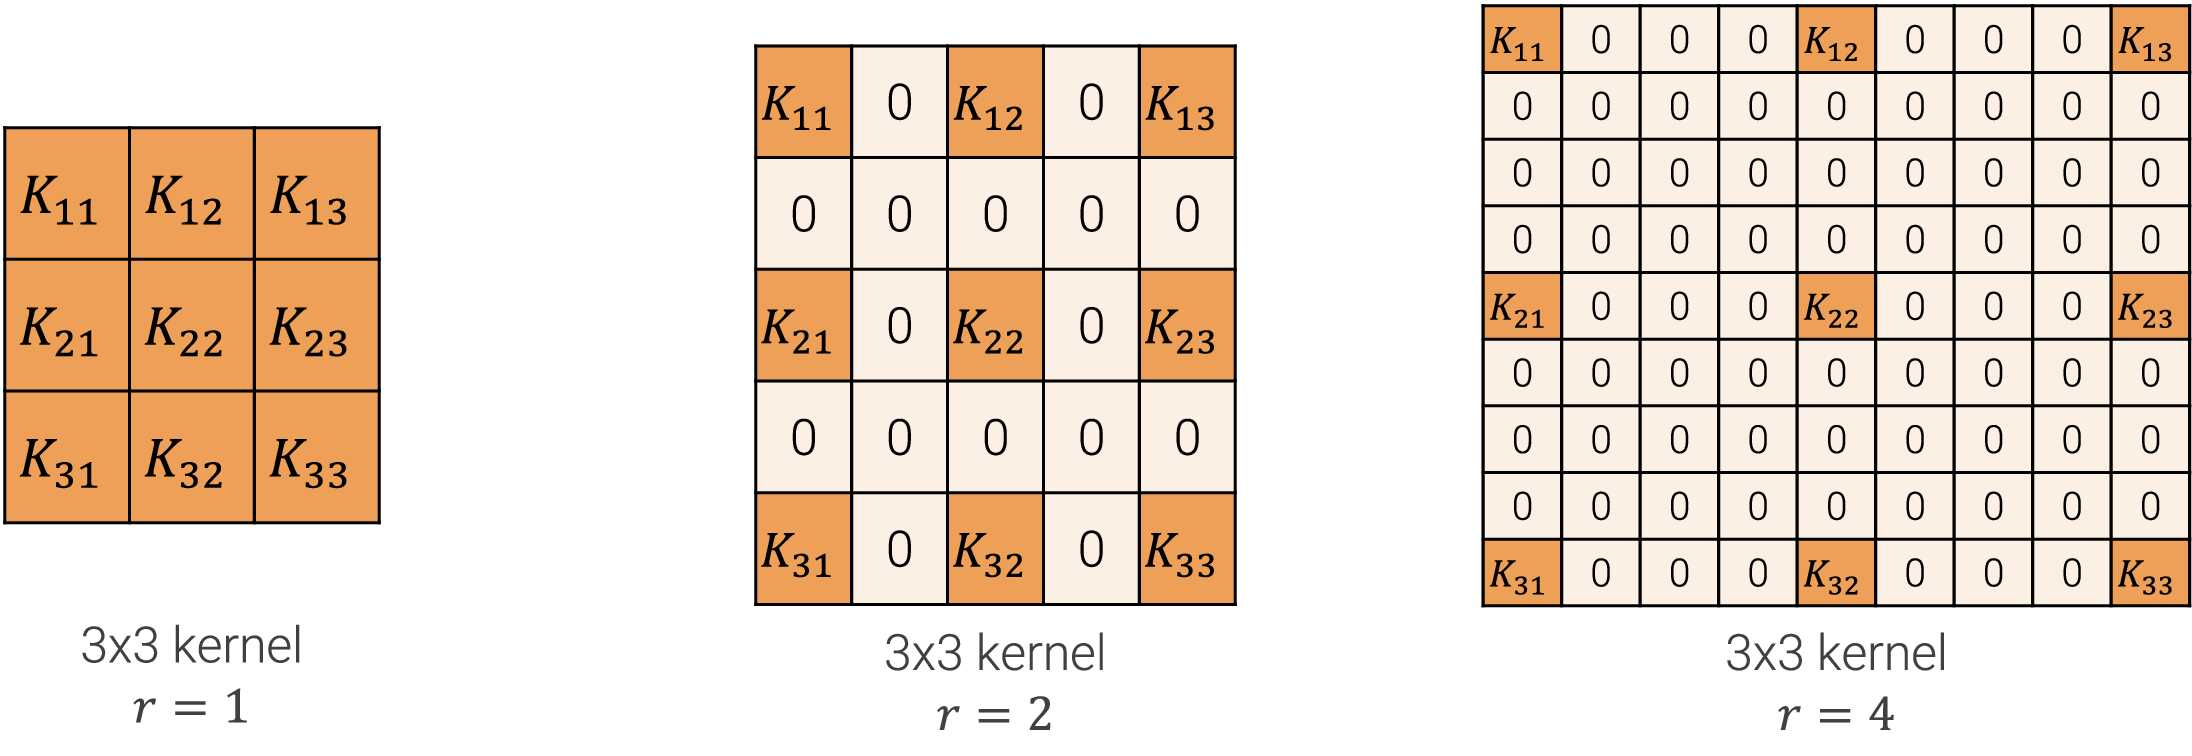
\includegraphics[width=0.7\linewidth]{./img/_dilated_convolution.jpg}
            \caption{Example of $3 \times 3$ dilated convolutions with increasing dilation rate}
        \end{figure}
        
        \begin{remark}
            By stacking dilated convolutions with exponentially increasing dilation rate $r_l = 2^l$, it is possible to achieve the following effects:
            \begin{itemize}
                \item Exponential growth in receptive field. At the $l$-th level the receptive field is $(2^{l+1} - 1) \times (2^{l+1} - 1)$.
                \item Linear growth in the number of parameters.
                \item Unchanged resolution.
            \end{itemize}

            \begin{figure}[H]
                \centering
                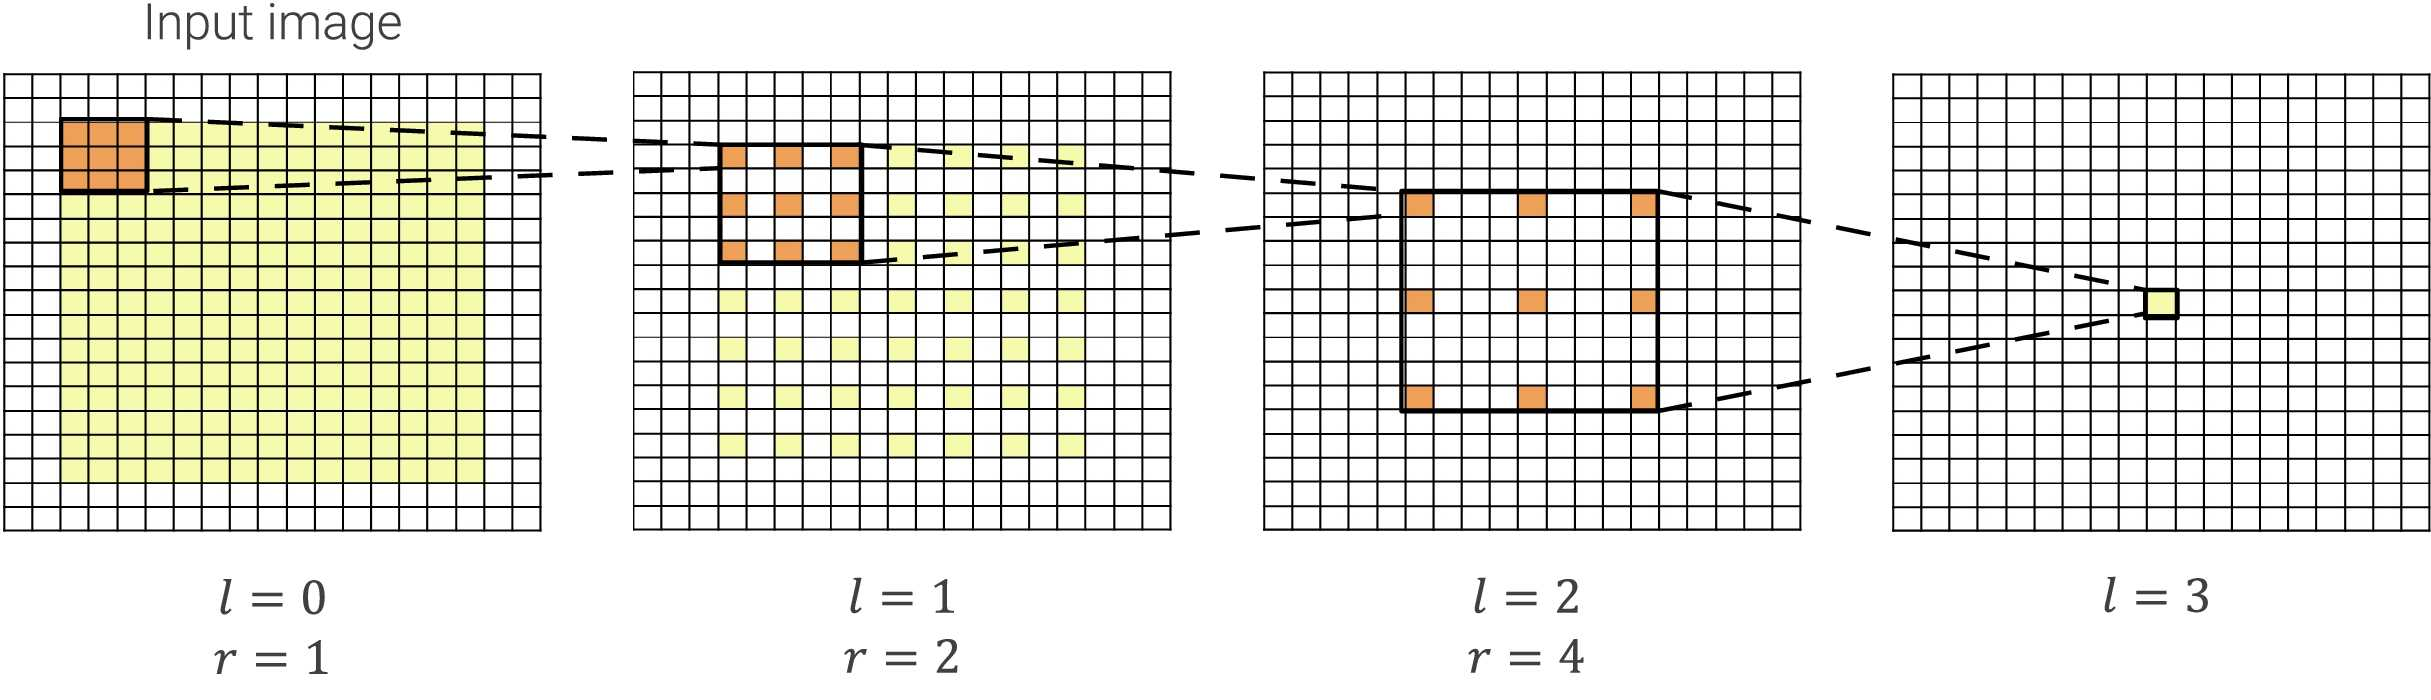
\includegraphics[width=0.9\linewidth]{./img/_dilated_convolution_exponential.jpg}
            \end{figure}
        \end{remark}

    \item[Dilated ResNet] \marginnote{Dilated ResNet}
        ResNet composed of standard stages up until a certain layer. The remaining ones are dilated stages.

        \begin{description}
            \item[Dilated bottleneck residual block]
                Standard bottleneck residual block composed of convolutions with kernels $1 \times 1 \mapsto 3 \times 3 \mapsto 1 \times 1$ where the middle $3 \times 3$ convolution is a dilated convolution.

            \item[Dilated stage]
                Given a dilation rate $r$, a dilated stage is built as follows:
                \begin{itemize}
                    \item The first bottleneck block has stride $1$ (instead of $2$) and dilation rate $\frac{r}{2}$.
                    \item The remaining blocks have stride $1$ and dilation rate $r$.
                \end{itemize}

                \begin{figure}[H]
                    \centering
                    \begin{subfigure}{0.45\linewidth}
                        \centering
                        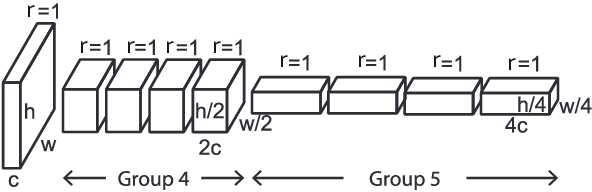
\includegraphics[width=0.9\linewidth]{./img/_dilated_resnet_stage1.jpg}
                        \caption{ResNet with standard stages}
                    \end{subfigure}
                    \begin{subfigure}{0.45\linewidth}
                        \centering
                        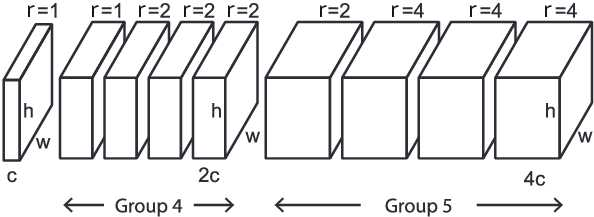
\includegraphics[width=0.9\linewidth]{./img/_dilated_resnet_stage2.jpg}
                        \caption{ResNet with two dilated stages}
                    \end{subfigure}
                \end{figure}
        \end{description}

        \begin{figure}[H]
            \centering
            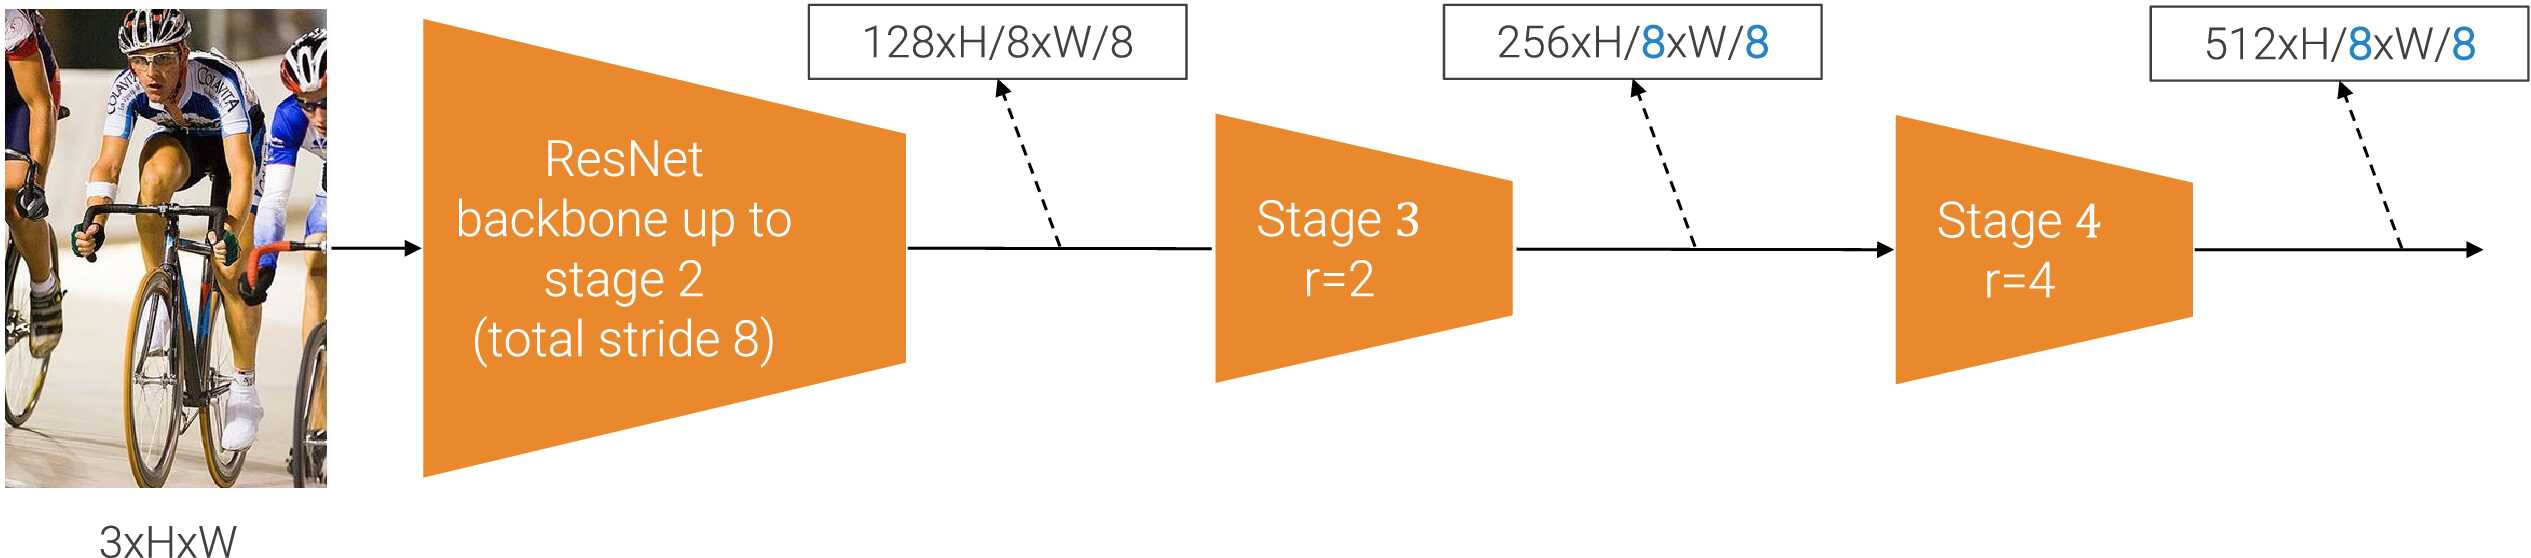
\includegraphics[width=0.9\linewidth]{./img/_dilated_resnet.jpg}
            \caption{Dilated ResNet with total stride $8$}
        \end{figure}

        \begin{remark}
            In principle, it is possible to process the input image without altering the resolution. However, this approach is computationally more expensive as the activations are larger. Therefore, the first standard ResNet stages are kept to apply some stride. As in FCN, a total stride of $8$ (up to the second stage) or $16$ (up to the third stage) is used.
        \end{remark}


    \item[DeepLab v3] \marginnote{DeepLab v3}
        Architecture based on dilated ResNet that considers objects at multiple scales.

        \begin{description}
            \item[Atrous spatial pyramid pooling (ASPP)] \marginnote{Atrous spatial pyramid pooling (ASPP)}
                Module that takes as input the activation of the dilated ResNet backbone and applies separate $3 \times 3$ convolutions with large dilation rates to encode spatial context. The final output is the concatenation of the activations of each convolution.

            \item[Curriculum training]
                Training is done in two steps:
                \begin{enumerate}
                    \item Train with a total stride of $16$ (i.e., only the last ResNet stage is dilated). This allows for a faster training with larger batches.
                    \item Fine-tune with a total stride of $8$ (i.e., the last two stages are dilated). This results in spatially larger and more detailed activations.
                \end{enumerate}
        \end{description}

        \begin{figure}[H]
            \centering
            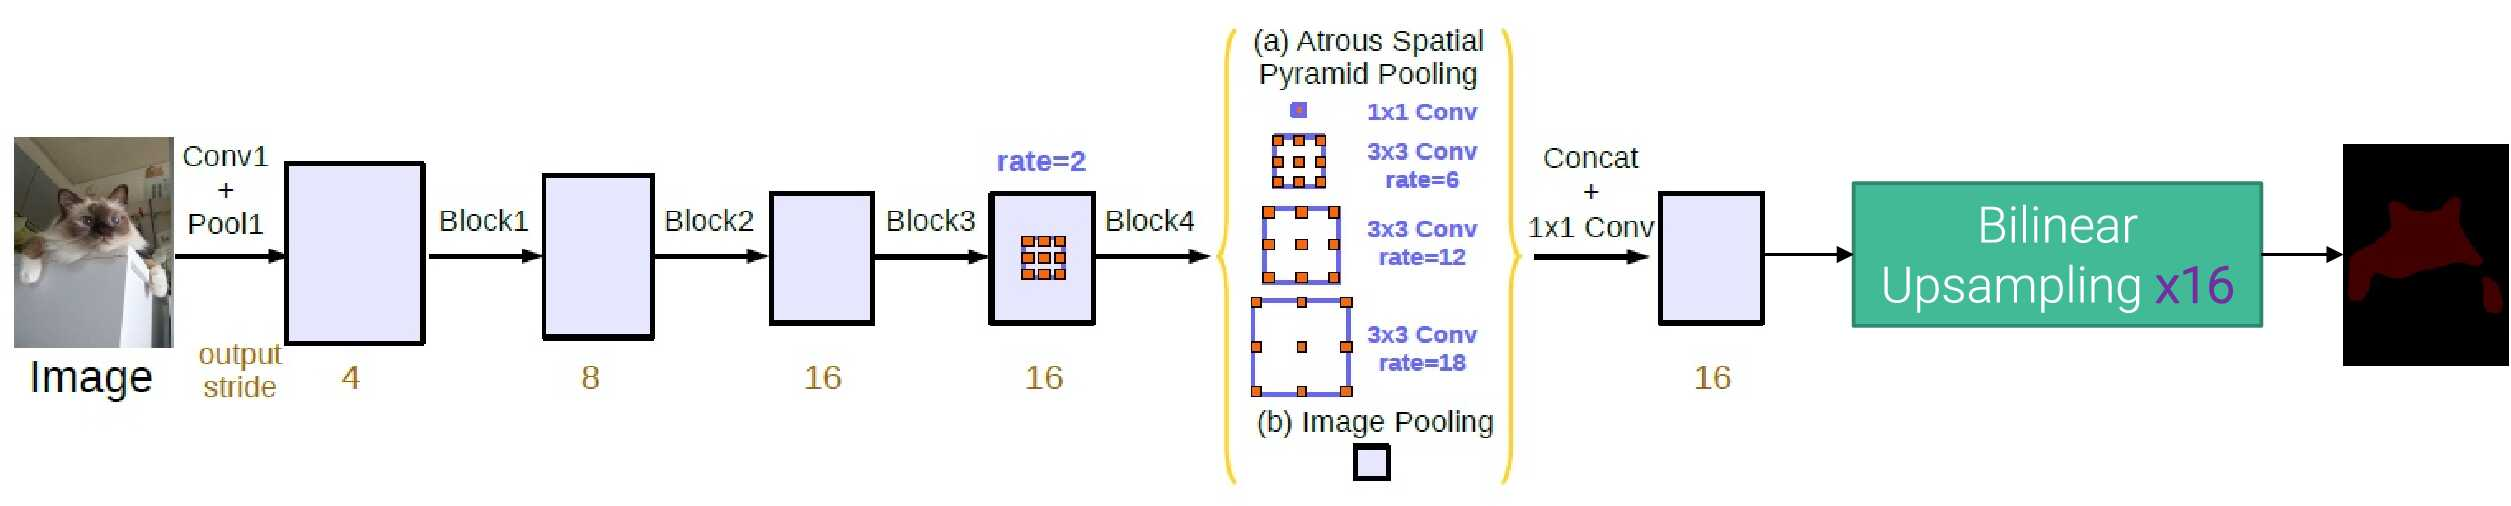
\includegraphics[width=0.95\linewidth]{./img/_deeplabv3.jpg}
        \end{figure}

    \item[DeepLab v3+] \marginnote{DeepLab v3+}
        Architecture based on the ASPP of DeepLab v3 and the decoder of U-Net.

        \begin{figure}[H]
            \centering
            \begin{subfigure}{0.3\linewidth}
                \centering
                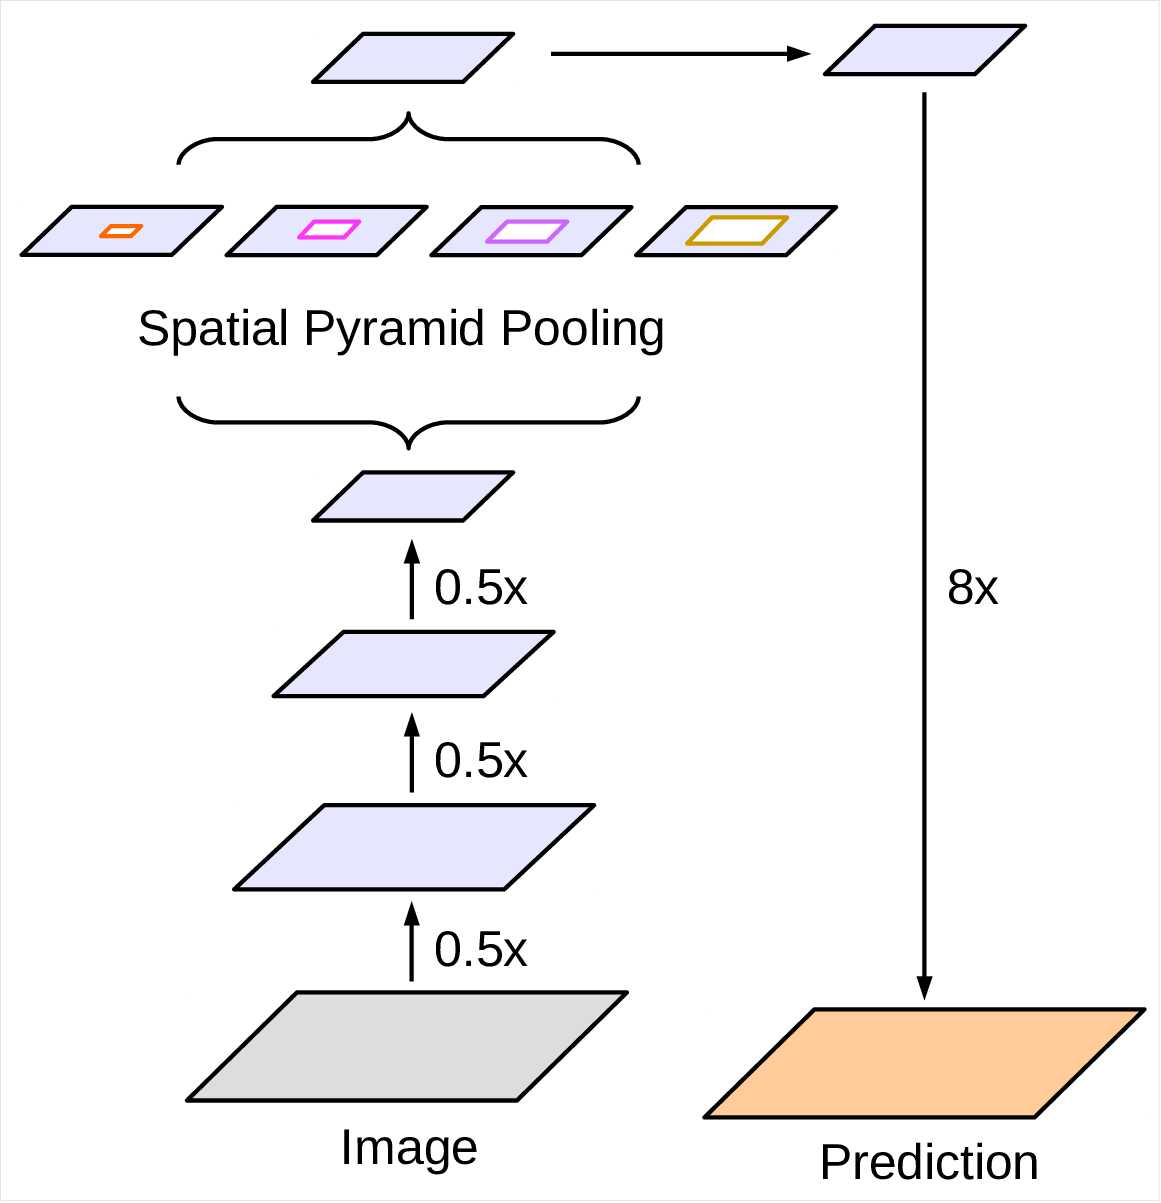
\includegraphics[width=0.9\linewidth]{./img/_deeplabv3plus_1.jpg}
                \caption{DeepLab v3}
            \end{subfigure}
            \begin{subfigure}{0.3\linewidth}
                \centering
                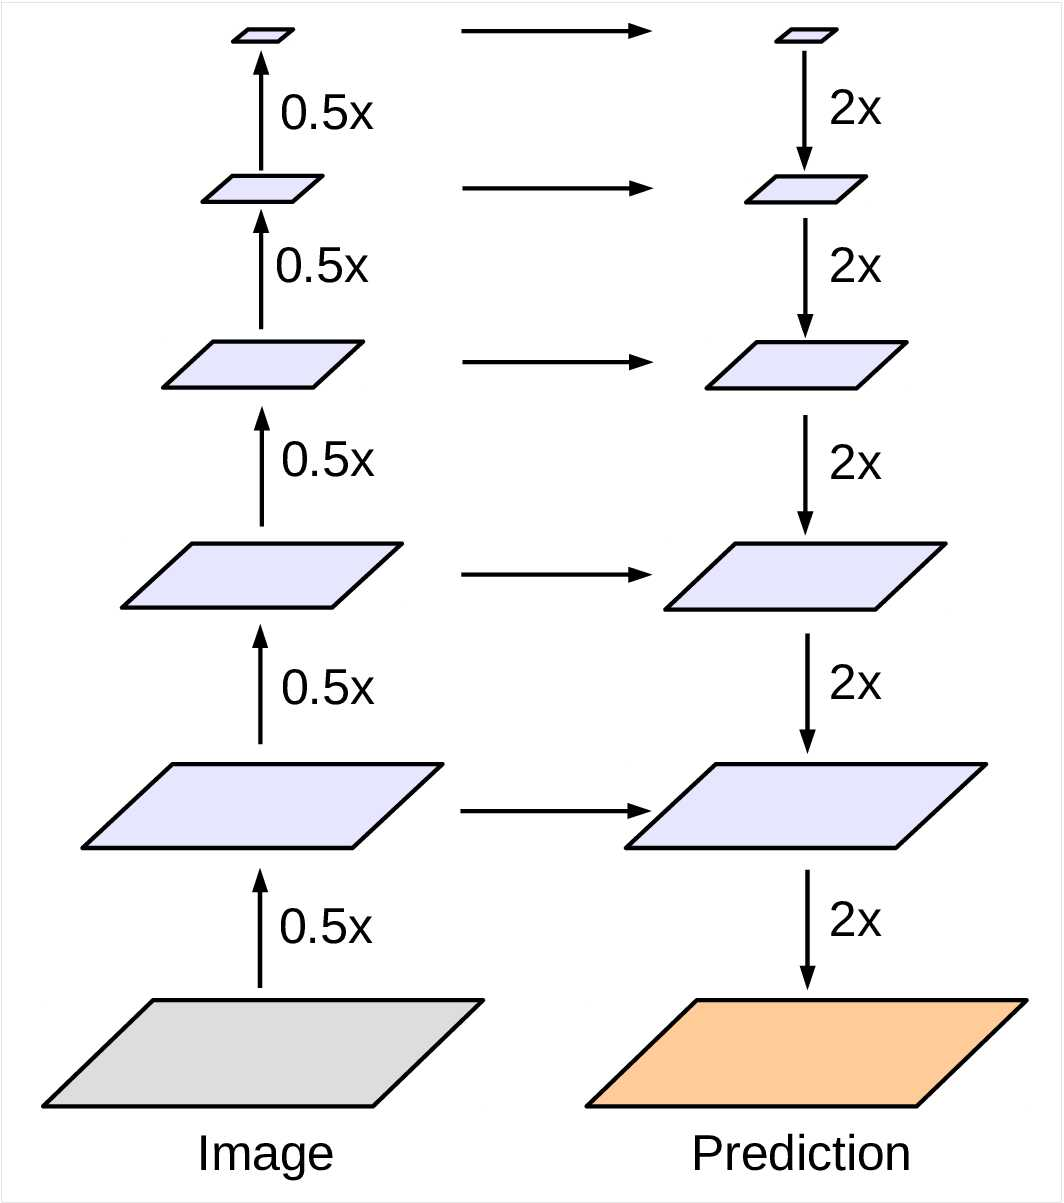
\includegraphics[width=0.9\linewidth]{./img/_deeplabv3plus_2.jpg}
                \caption{U-Net}
            \end{subfigure}
            \hfill
            \begin{subfigure}{0.3\linewidth}
                \centering
                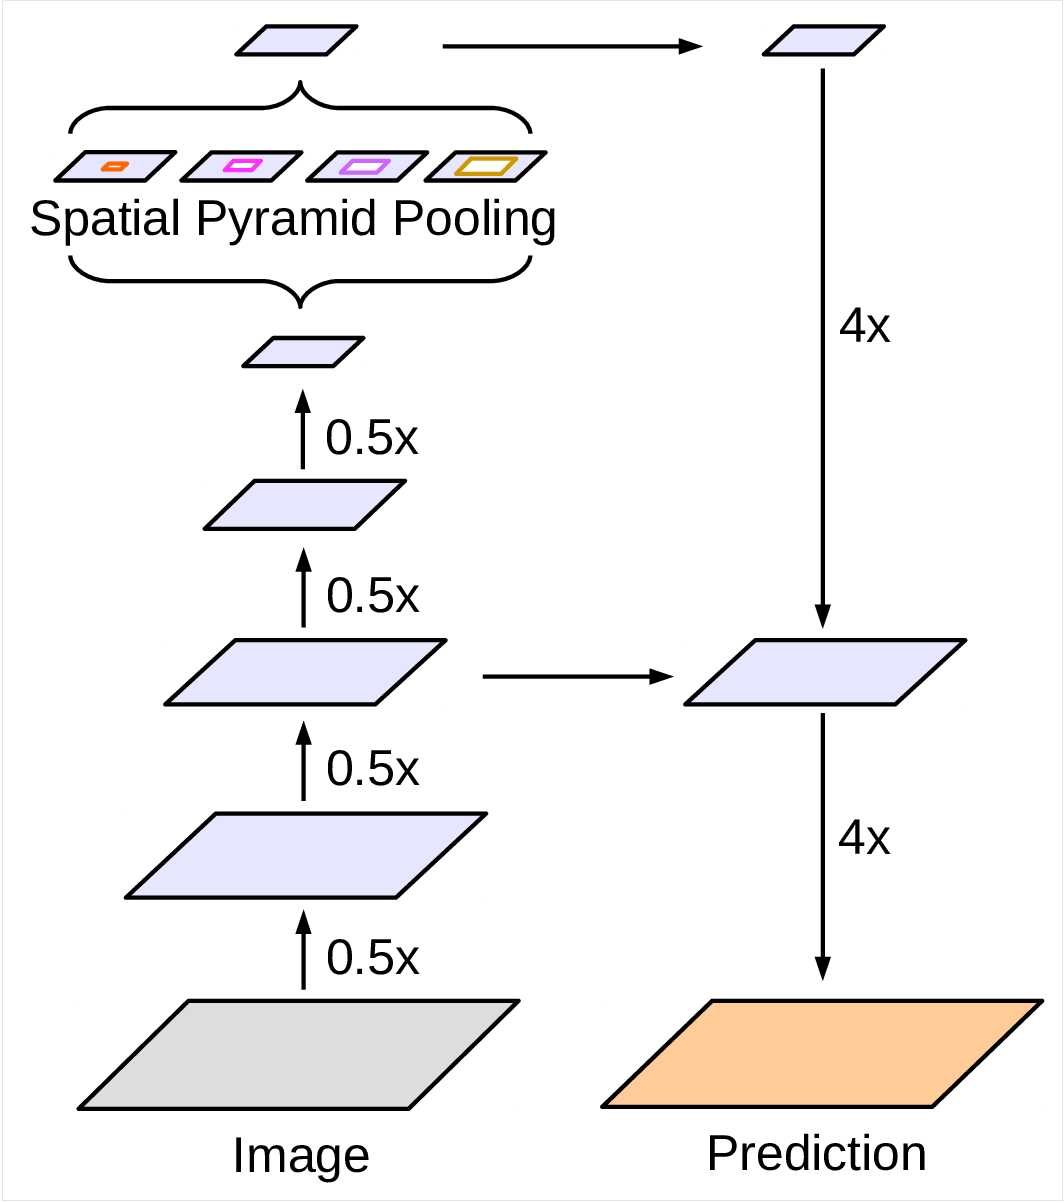
\includegraphics[width=0.9\linewidth]{./img/_deeplabv3plus_3.jpg}
                \caption{DeepLab v3+}
            \end{subfigure}
        \end{figure}
\end{description}



\section{Instance segmentation}

\begin{description}
    \item[Instance segmentation] \marginnote{Instance segmentation}
        Task of segmenting and classifying all instances of the objects of interest (i.e., intersection between object detection and semantic segmentation).

        \begin{figure}[H]
            \centering
            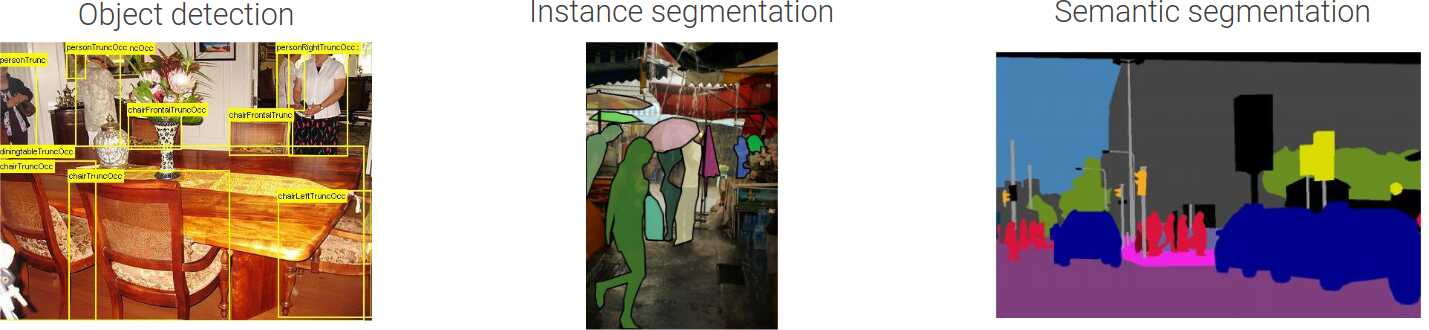
\includegraphics[width=0.7\linewidth]{./img/obj_detection_and_segmentation.jpg}
        \end{figure}
\end{description}


\subsection{Mask R-CNN}

\begin{description}
    \item[Mask R-CNN] \marginnote{Mask R-CNN}
        Architecture based on faster R-CNN with a modification to RoI pool and the addition of a CNN head to predict the segmentation mask.

        \begin{description}
            \item[RoI align] \marginnote{RoI align}
                Modification to RoI pool to avoid quantization. It works as follows:
                \begin{enumerate}
                    \item Divide the proposal into equal subregions without snapping to grid.
                    \begin{figure}[H]
                        \centering
                        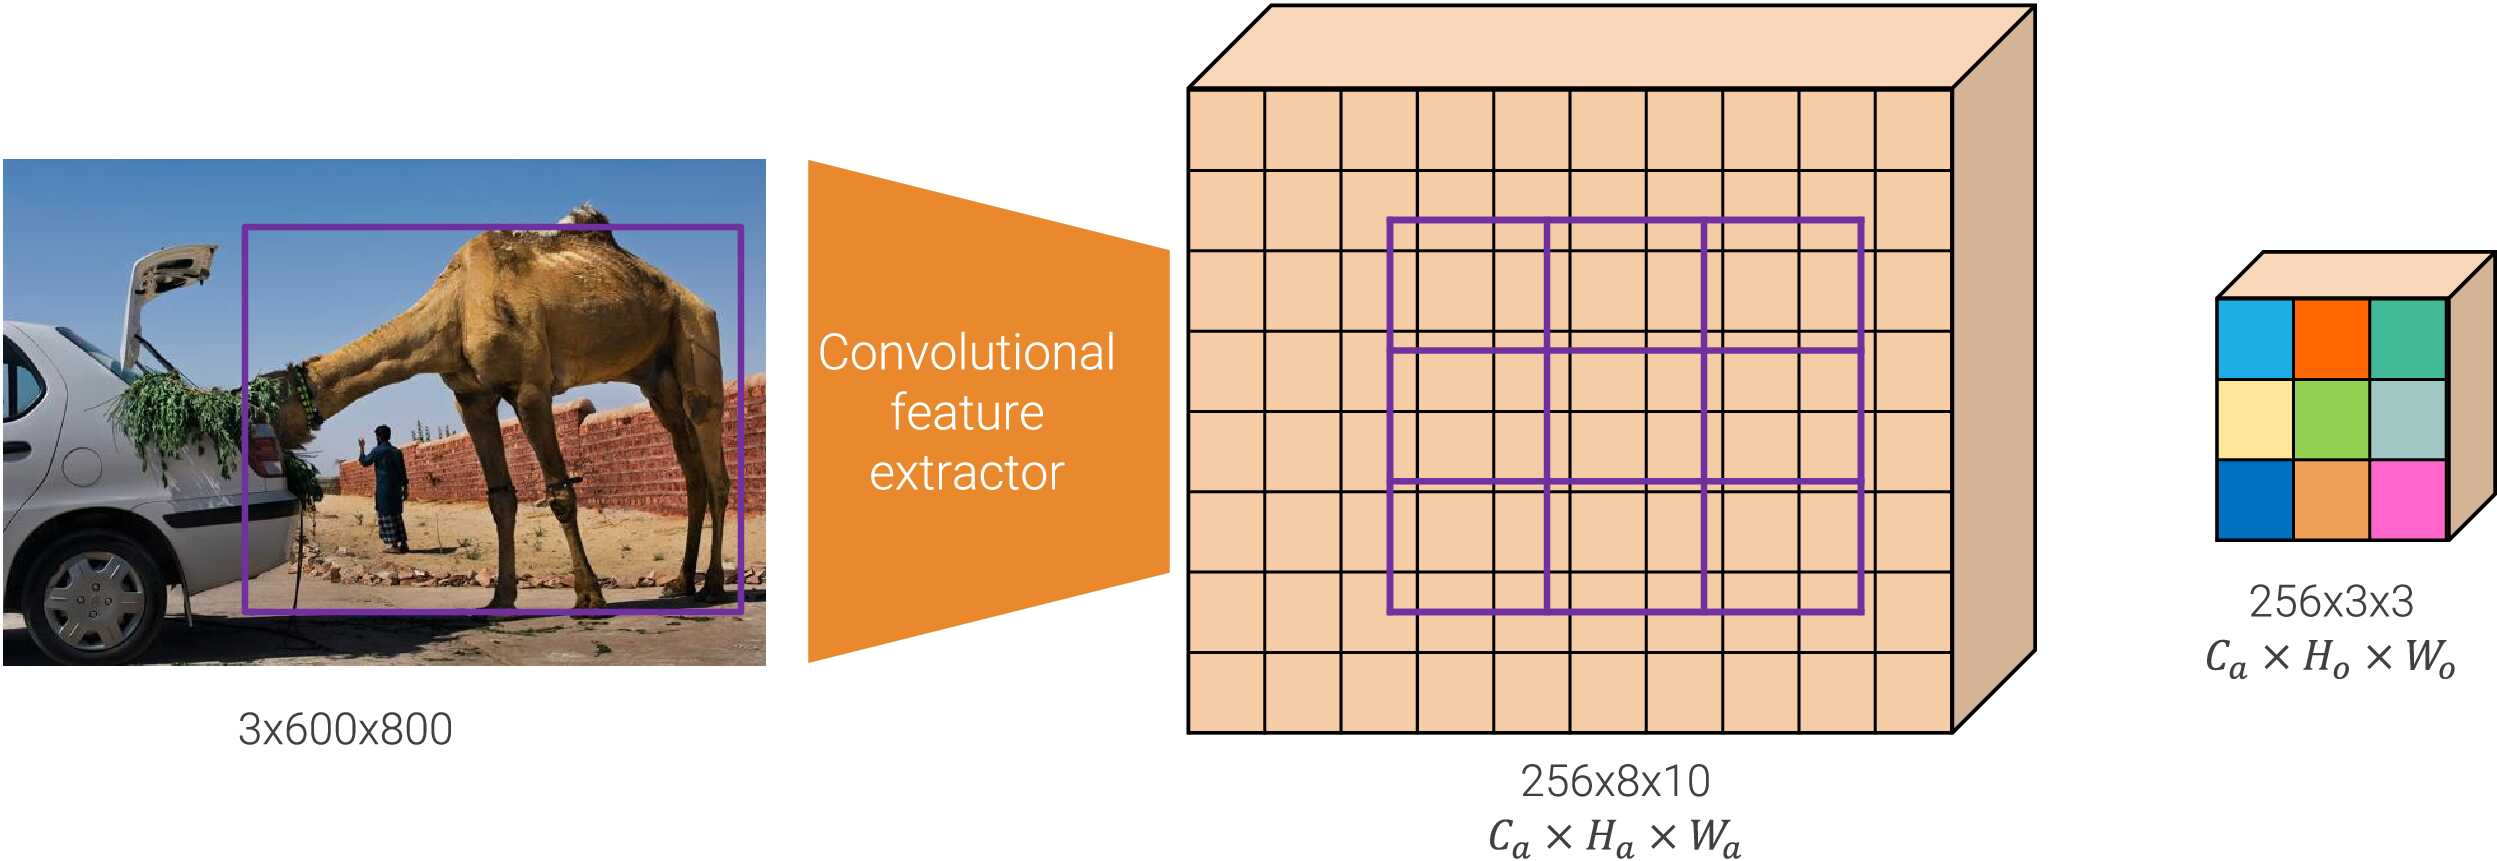
\includegraphics[width=0.7\linewidth]{./img/_roi_align1.jpg}
                    \end{figure}
                    \item Sample some values following a regular grid within each subregion. Use bilinear interpolation to determine the values of the sampled points (as they are most likely not pixel-perfect).
                    \begin{figure}[H]
                        \centering
                        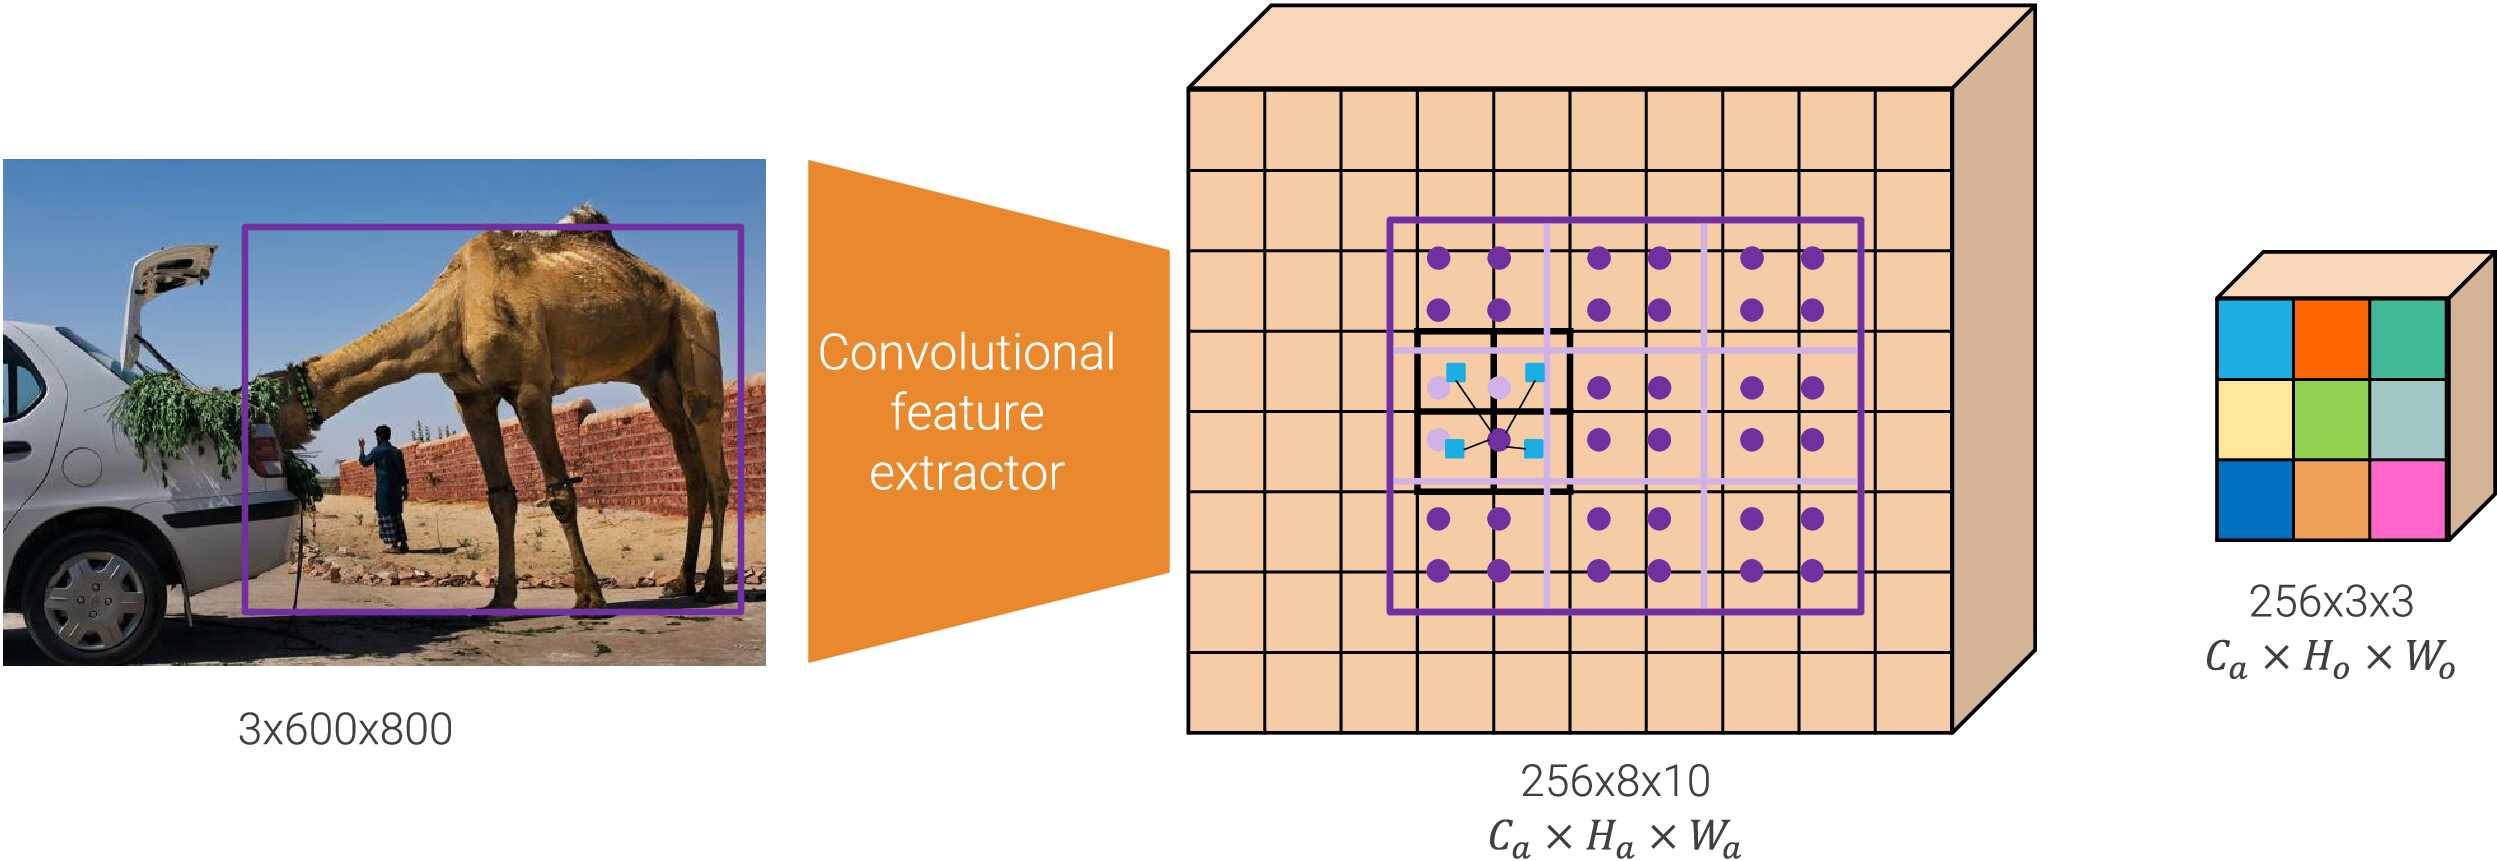
\includegraphics[width=0.7\linewidth]{./img/_roi_align2.jpg}
                    \end{figure}
                    \item Max or average pool the sampled values in each subregion.
                    \begin{figure}[H]
                        \centering
                        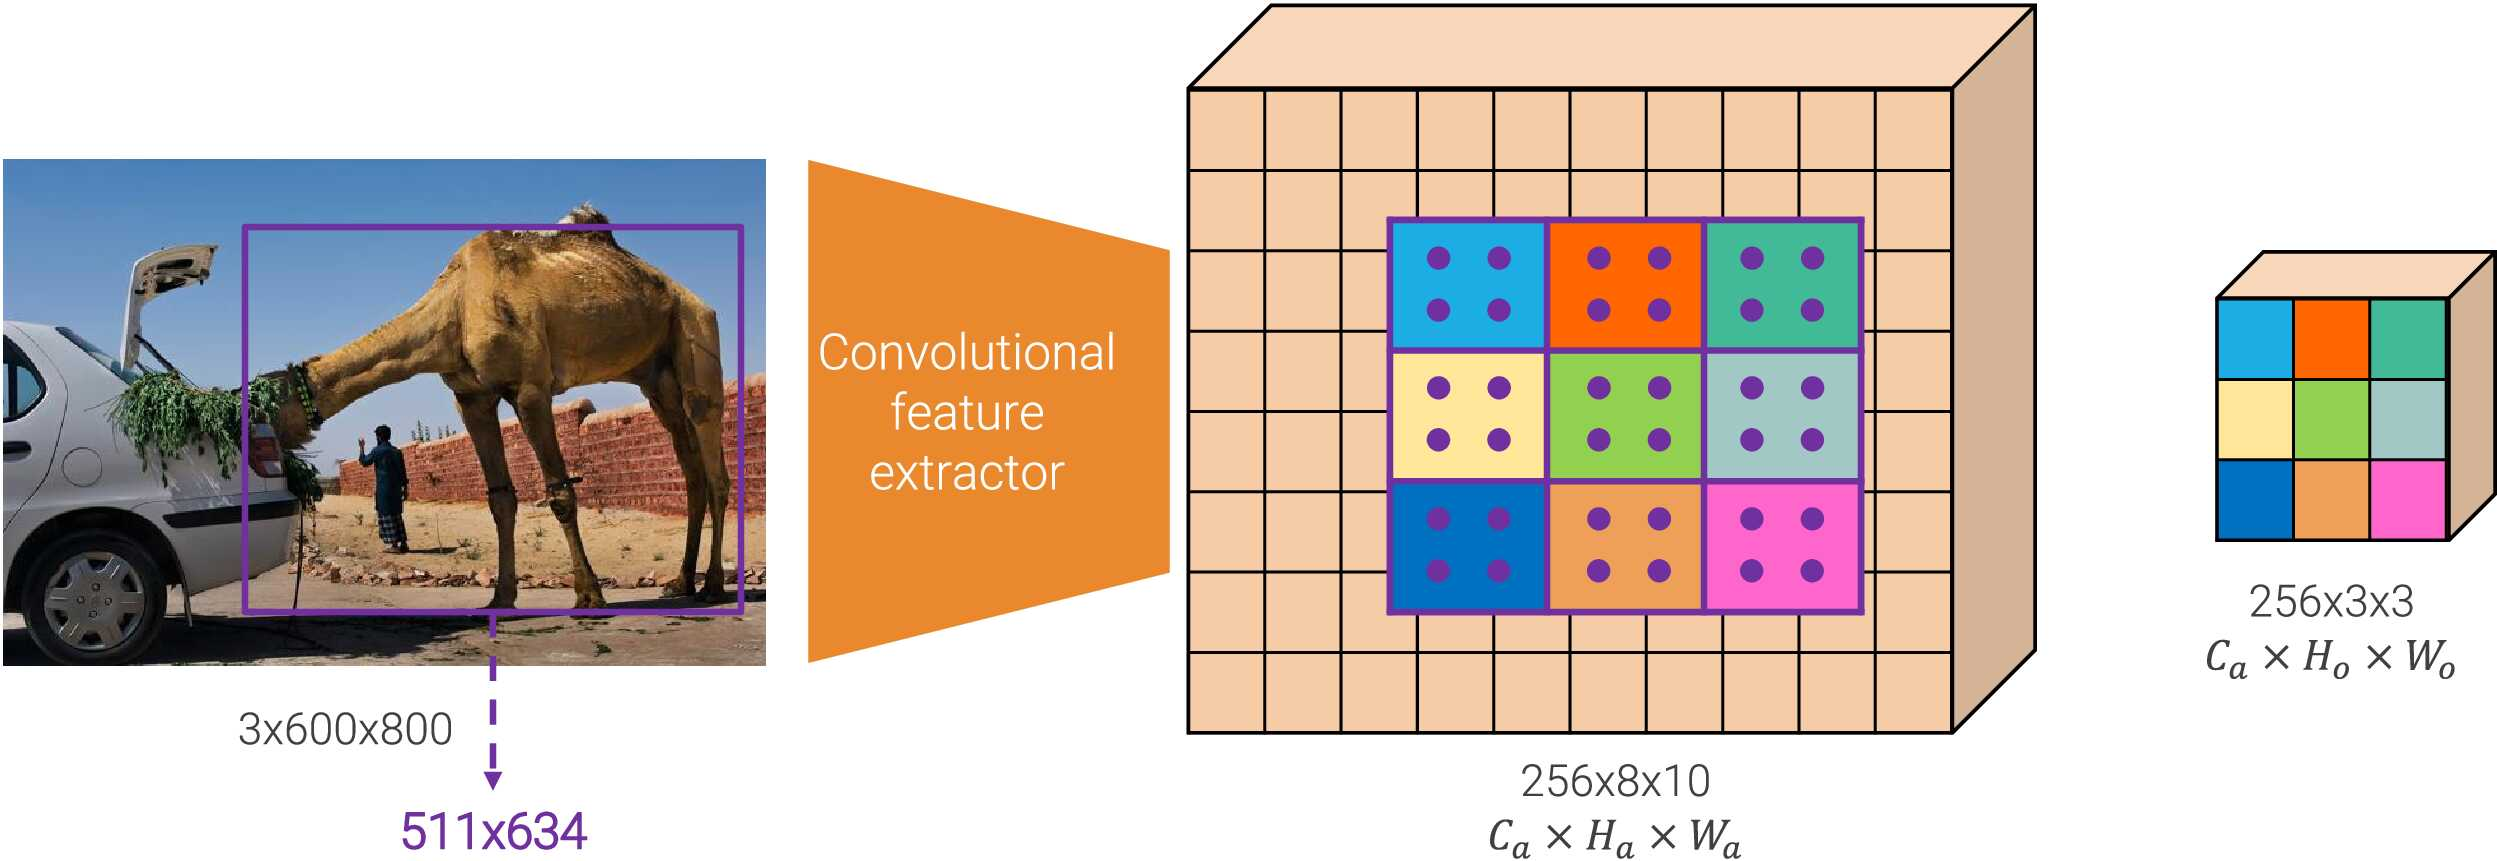
\includegraphics[width=0.7\linewidth]{./img/_roi_align3.jpg}
                    \end{figure}
                \end{enumerate}

            \item[Mask head] \marginnote{Mask head}
                Fully-convolutional network that takes the output of RoI align and predicts a binary mask with resolution $28 \times 28$ for each class. It is composed of convolutions, a transposed convolution, and a scoring layer.

                In practice, the bounding box predicted by the standard R-CNN flow is used to determine how to warp the segmentation mask onto the original image.

                \begin{remark}
                    Empirical experiments show that solving a multi-label problem (i.e., multiple sigmoids) is better than a multi-class problem (i.e., softmax).
                \end{remark}

                \begin{figure}[H]
                    \centering
                    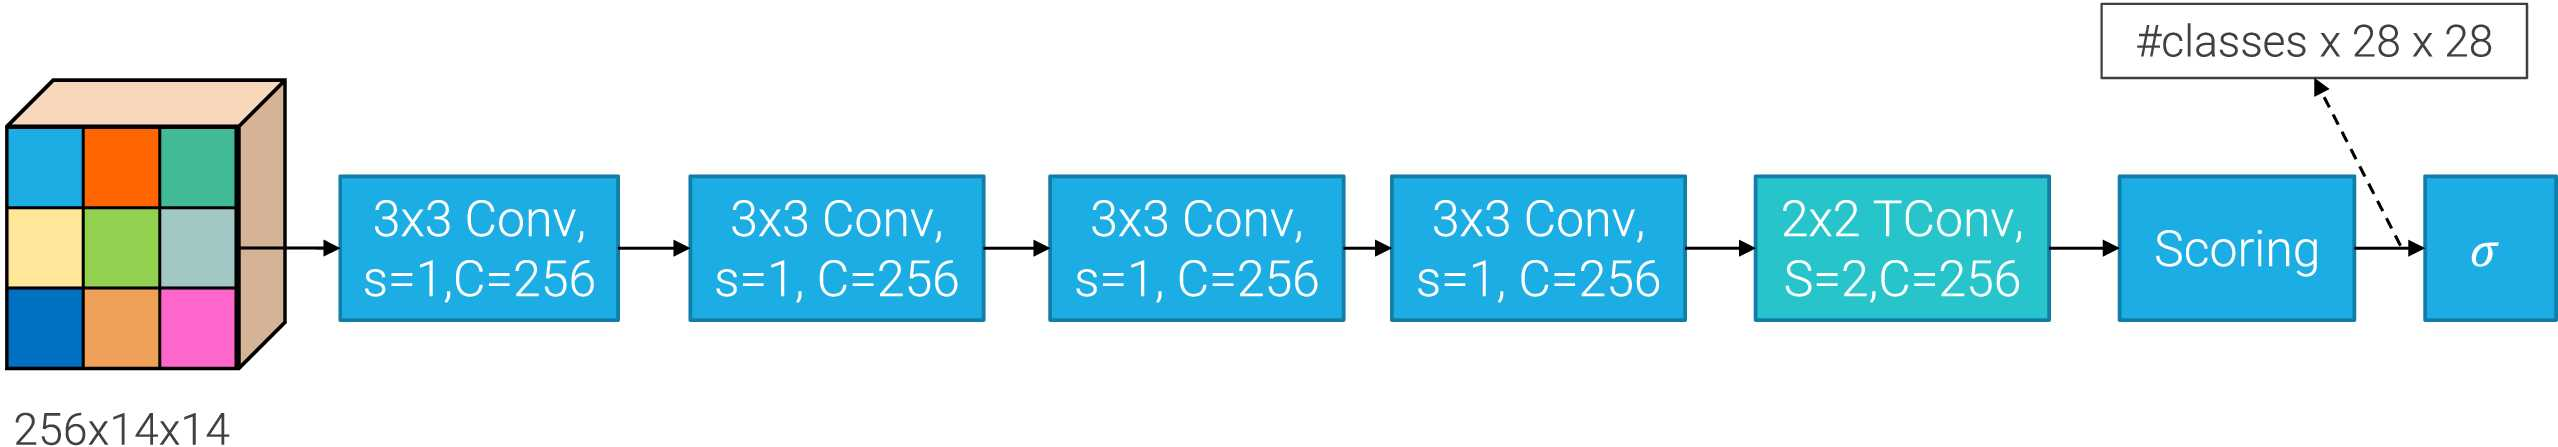
\includegraphics[width=0.85\linewidth]{./img/_mask_rcnn_head.jpg}
                \end{figure}
        \end{description}

        \begin{figure}[H]
            \centering
            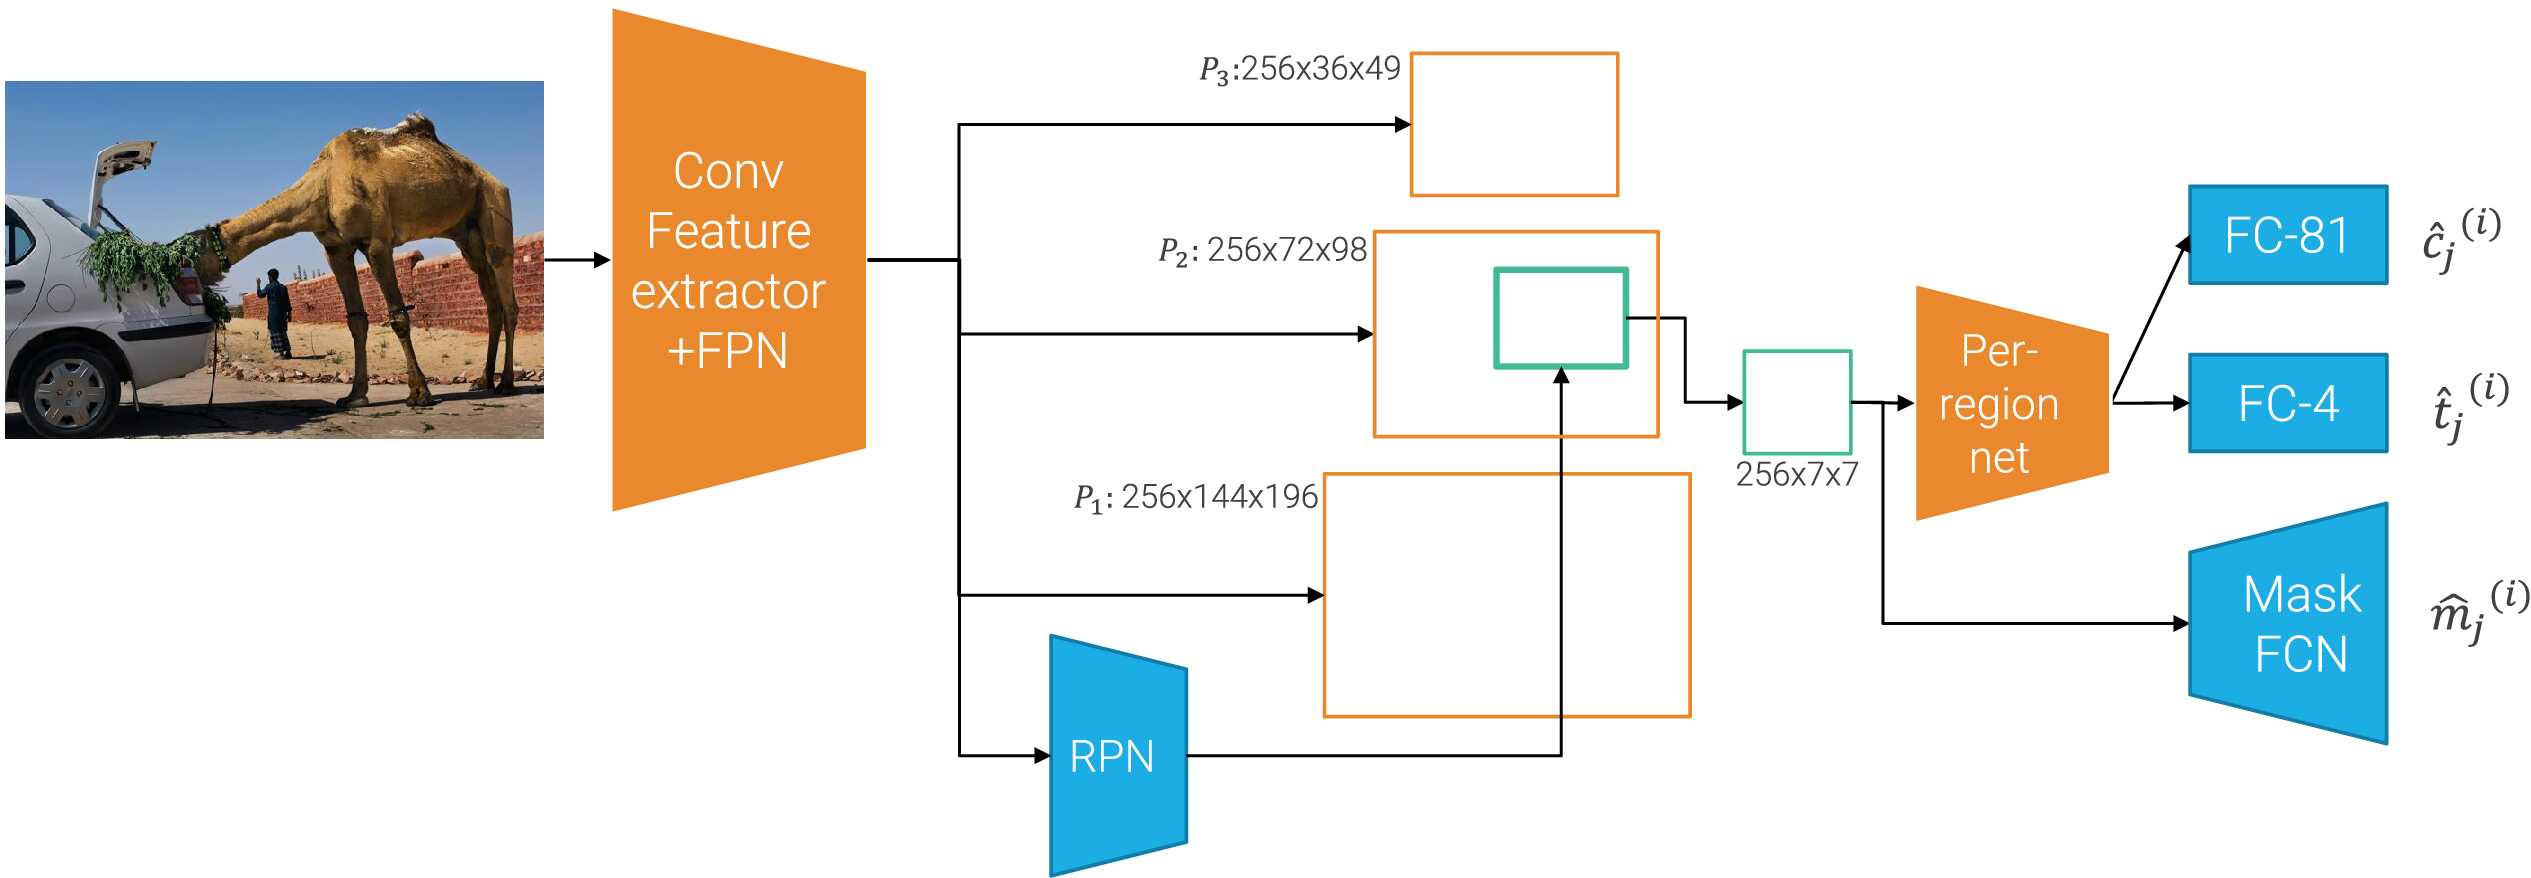
\includegraphics[width=0.85\linewidth]{./img/_mask_rcnn.jpg}
            \caption{Overall architecture of mask R-CNN}
        \end{figure}

        \begin{description}
        \item[Training]
            The R-CNN flow is trained in the standard way. 

            Given the ground-truth class $c$ and mask $m$, and the predicted mask $\hat{m}$, the mask head is trained using the following loss:
            \[ \mathcal{L}_\text{mask}(c, m) = \frac{1}{28 \times 28} \sum_{u=0}^{27} \sum_{v=0}^{27} \mathcal{L}_\text{BCE}\left( \hat{m}_{c}[u, v], m[u, v] \right) \]
            In other words, the ground-truth mask is compared against the predicted mask at the correct class.

        \item[Inference]
            The class prediction of R-CNN is used to select the correct channel of the mask head. The bounding box of R-CNN is used to decide how to warp the segmentation mask onto the image.
    \end{description}
\end{description}

\begin{remark}
    By attaching a different head to predict keypoints, this framework can be adapted for human pose estimation.
\end{remark}



\section{Panoptic segmentation}

\begin{description}
    \item[Things] \marginnote{Things}
        Countable object categories that can be split into individual instances.

    \item[Stuff] \marginnote{Stuff}
        Uncountable amorphous regions (e.g., background)

    \item[Panoptic segmentation] \marginnote{Panoptic segmentation}
        Task of classifying each pixel of the image. Objects of interest (i.e., things) are treated as in instance segmentation. Background and non-relevant textures (i.e., stuff) are treated as in semantic segmentation.

        \begin{figure}[H]
            \centering
            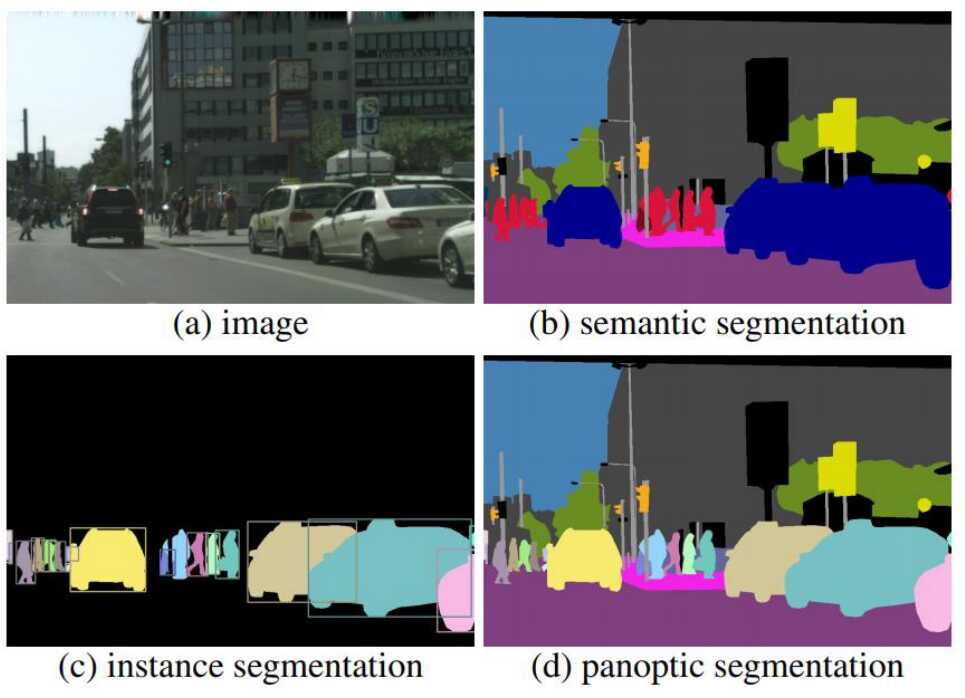
\includegraphics[width=0.5\linewidth]{./img/segmentation_types.jpg}
        \end{figure}
\end{description}


\subsection{Panoptic feature pyramid network}

\begin{description}
    \item[Panoptic feature pyramid network] \marginnote{Panoptic feature pyramid network}
        Modification of mask R-CNN with an additional path for stuff prediction that works as follows:
        \begin{enumerate}
            \item Rescale and merge FPN feature maps.
            \item Pass the result through a fully-convolutional network to predict stuff masks.
        \end{enumerate}

        When generating the predictions, the mask head (for things prediction) has the priority over the stuff head.

        \begin{figure}[H]
            \centering
            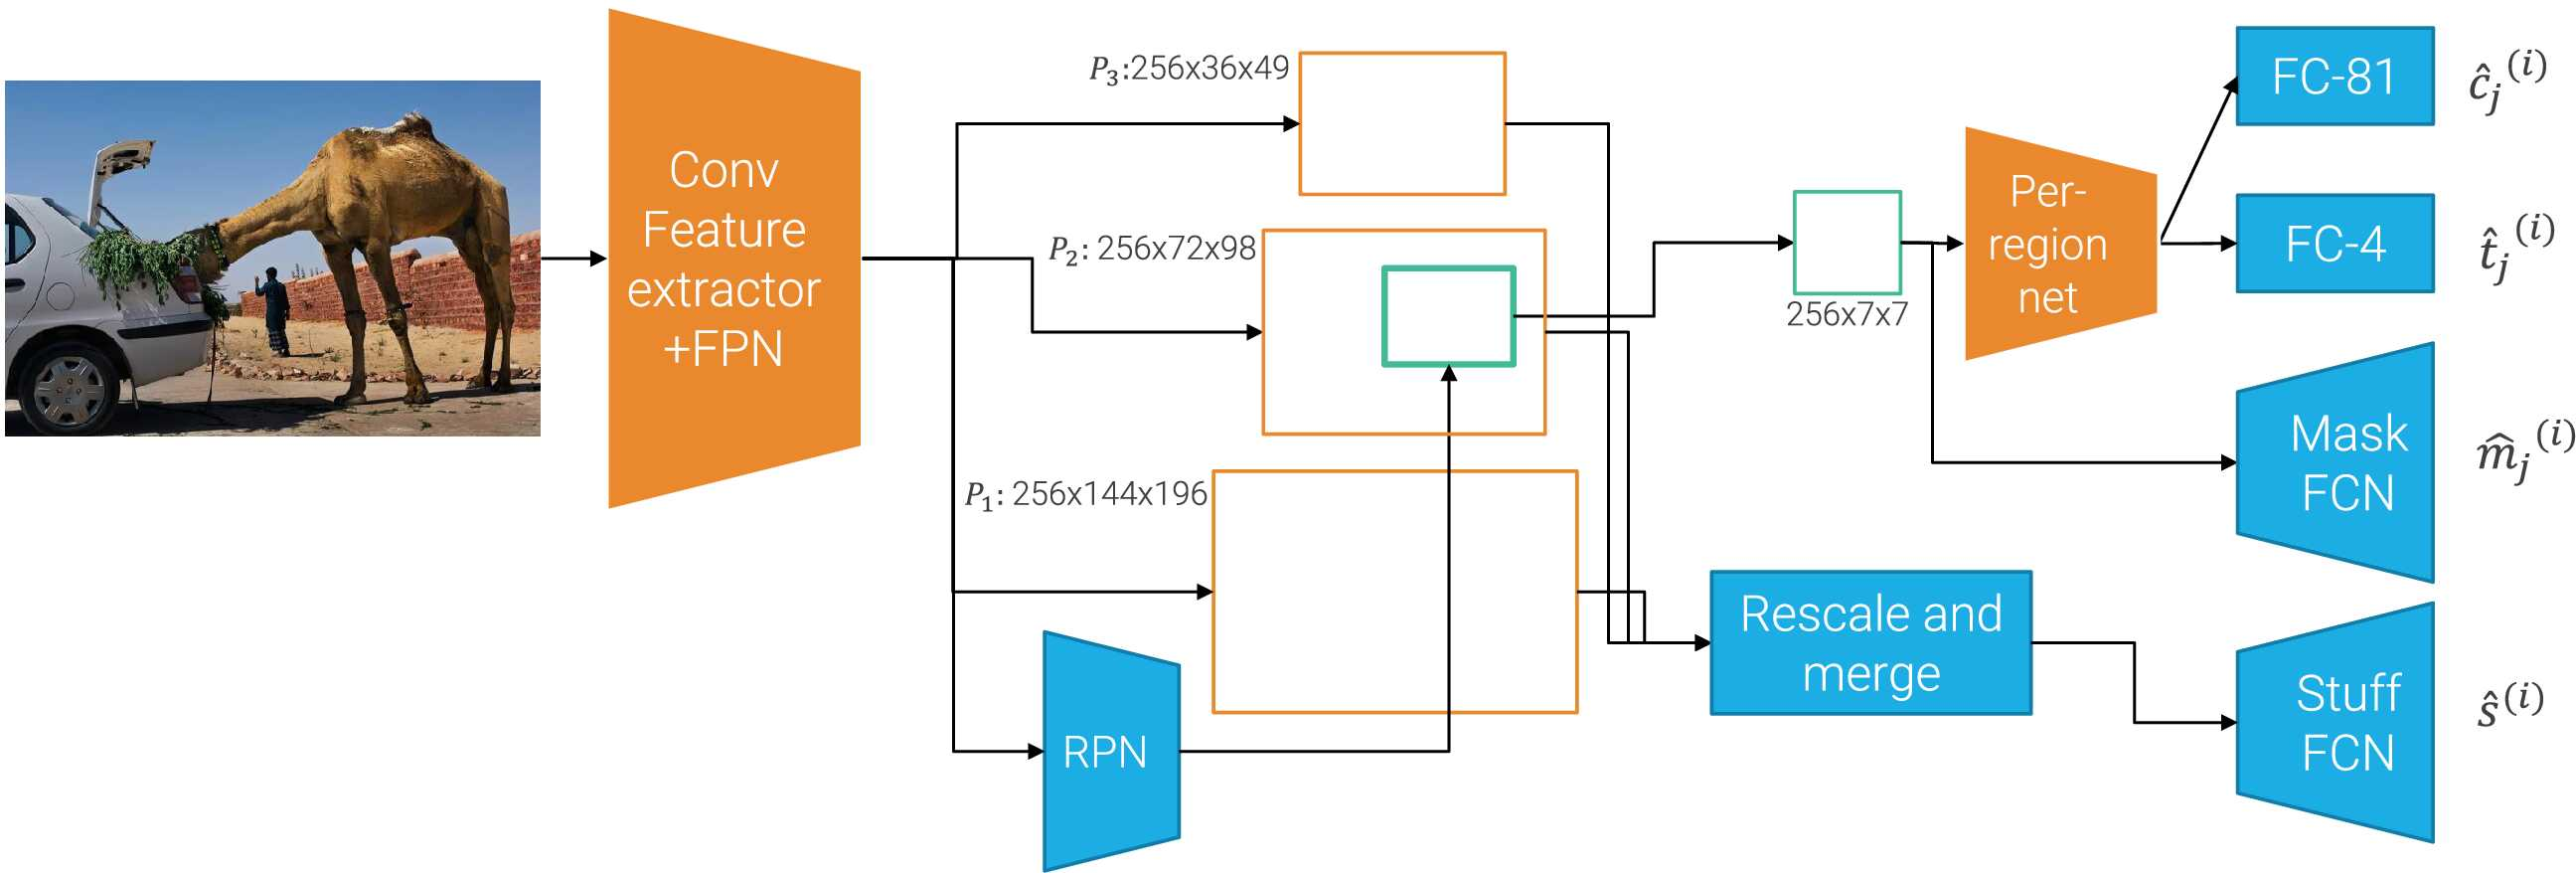
\includegraphics[width=0.85\linewidth]{./img/_panoptic_fpn.jpg}
        \end{figure}
\end{description}


\subsection{MaskFormer}

\begin{remark}
    With convolutions, semantic segmentation has been solved by classifying each pixel into a class. On the other hand, instance and panoptic segmentation partition the image into masks and classify them.

    It is intuitive to show that solving a mask classification problem can solve all types of segmentation.
\end{remark}

\begin{description}
    \item[MaskFormer] \marginnote{MaskFormer}
        Modification of DETR for pixel-wise predictions.

        \begin{description}
            \item[Architecture (naive)] 
                An additional path is inserted at the output of the transformer decoder that passes each of its output into a multi layer perceptron to predict a binary mask.

                \begin{remark}
                    This approach attempts to predict full-resolution masks from spatially coarse features.
                \end{remark}

                \begin{figure}[H]
                    \centering
                    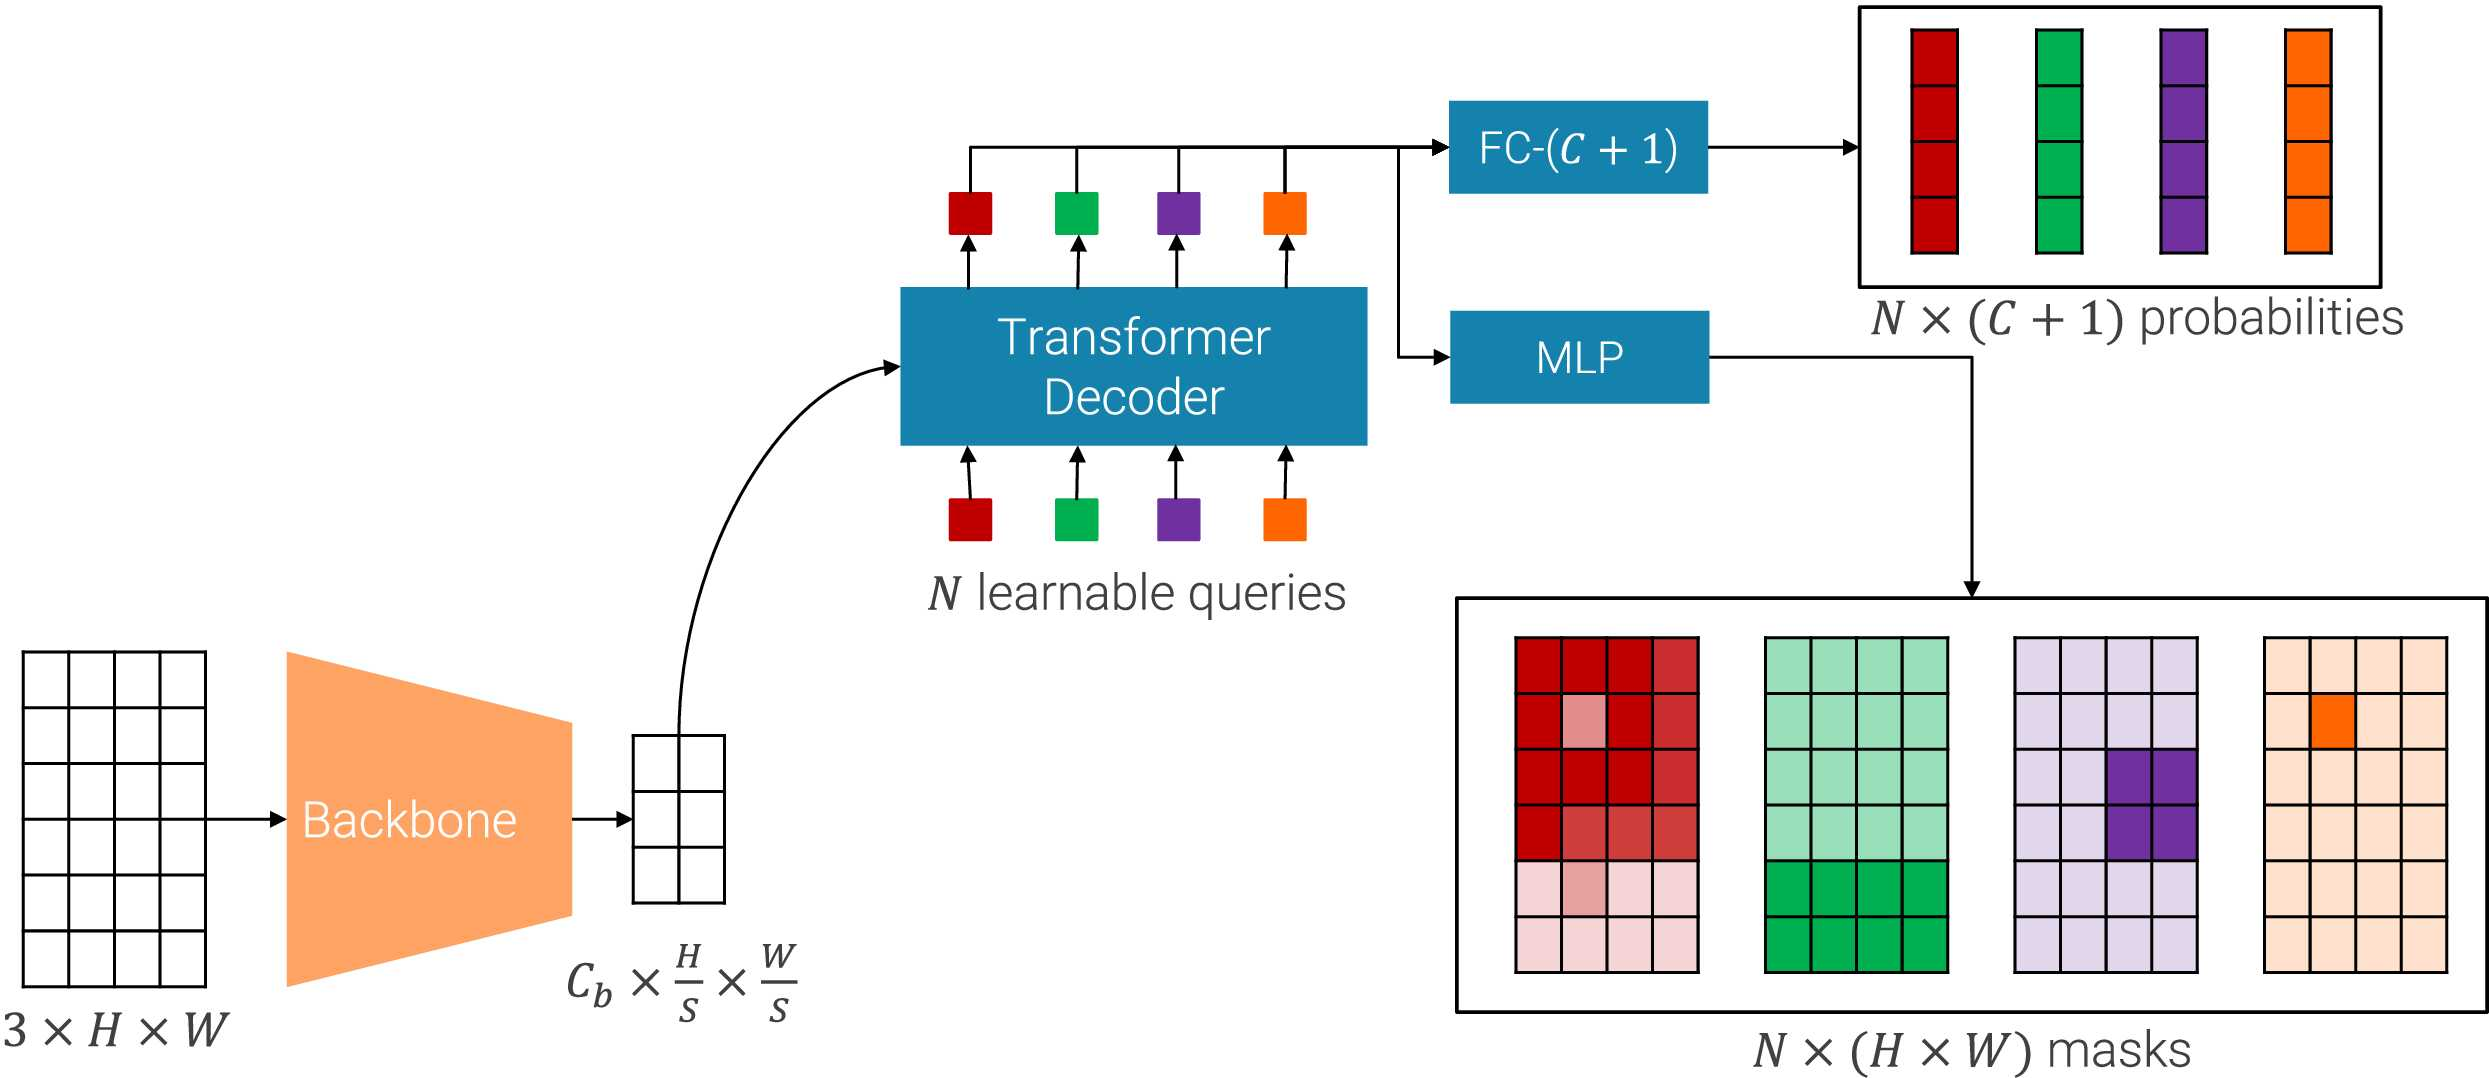
\includegraphics[width=0.75\linewidth]{./img/_maskformer_naive.jpg}
                \end{figure}

            \item[Architecture (pixel decoder)] 
                The following operations are added:
                \begin{enumerate}
                    \item A pixel decoder is used to compute pixel-wise embeddings from the output of the CNN backbone.
                    \item An MLP is added to compute mask embeddings from the outputs of the transformer decoder.
                    \item The dot product between mask and pixel embeddings allows to compute the output binary masks.
                \end{enumerate}

                \begin{figure}[H]
                    \centering
                    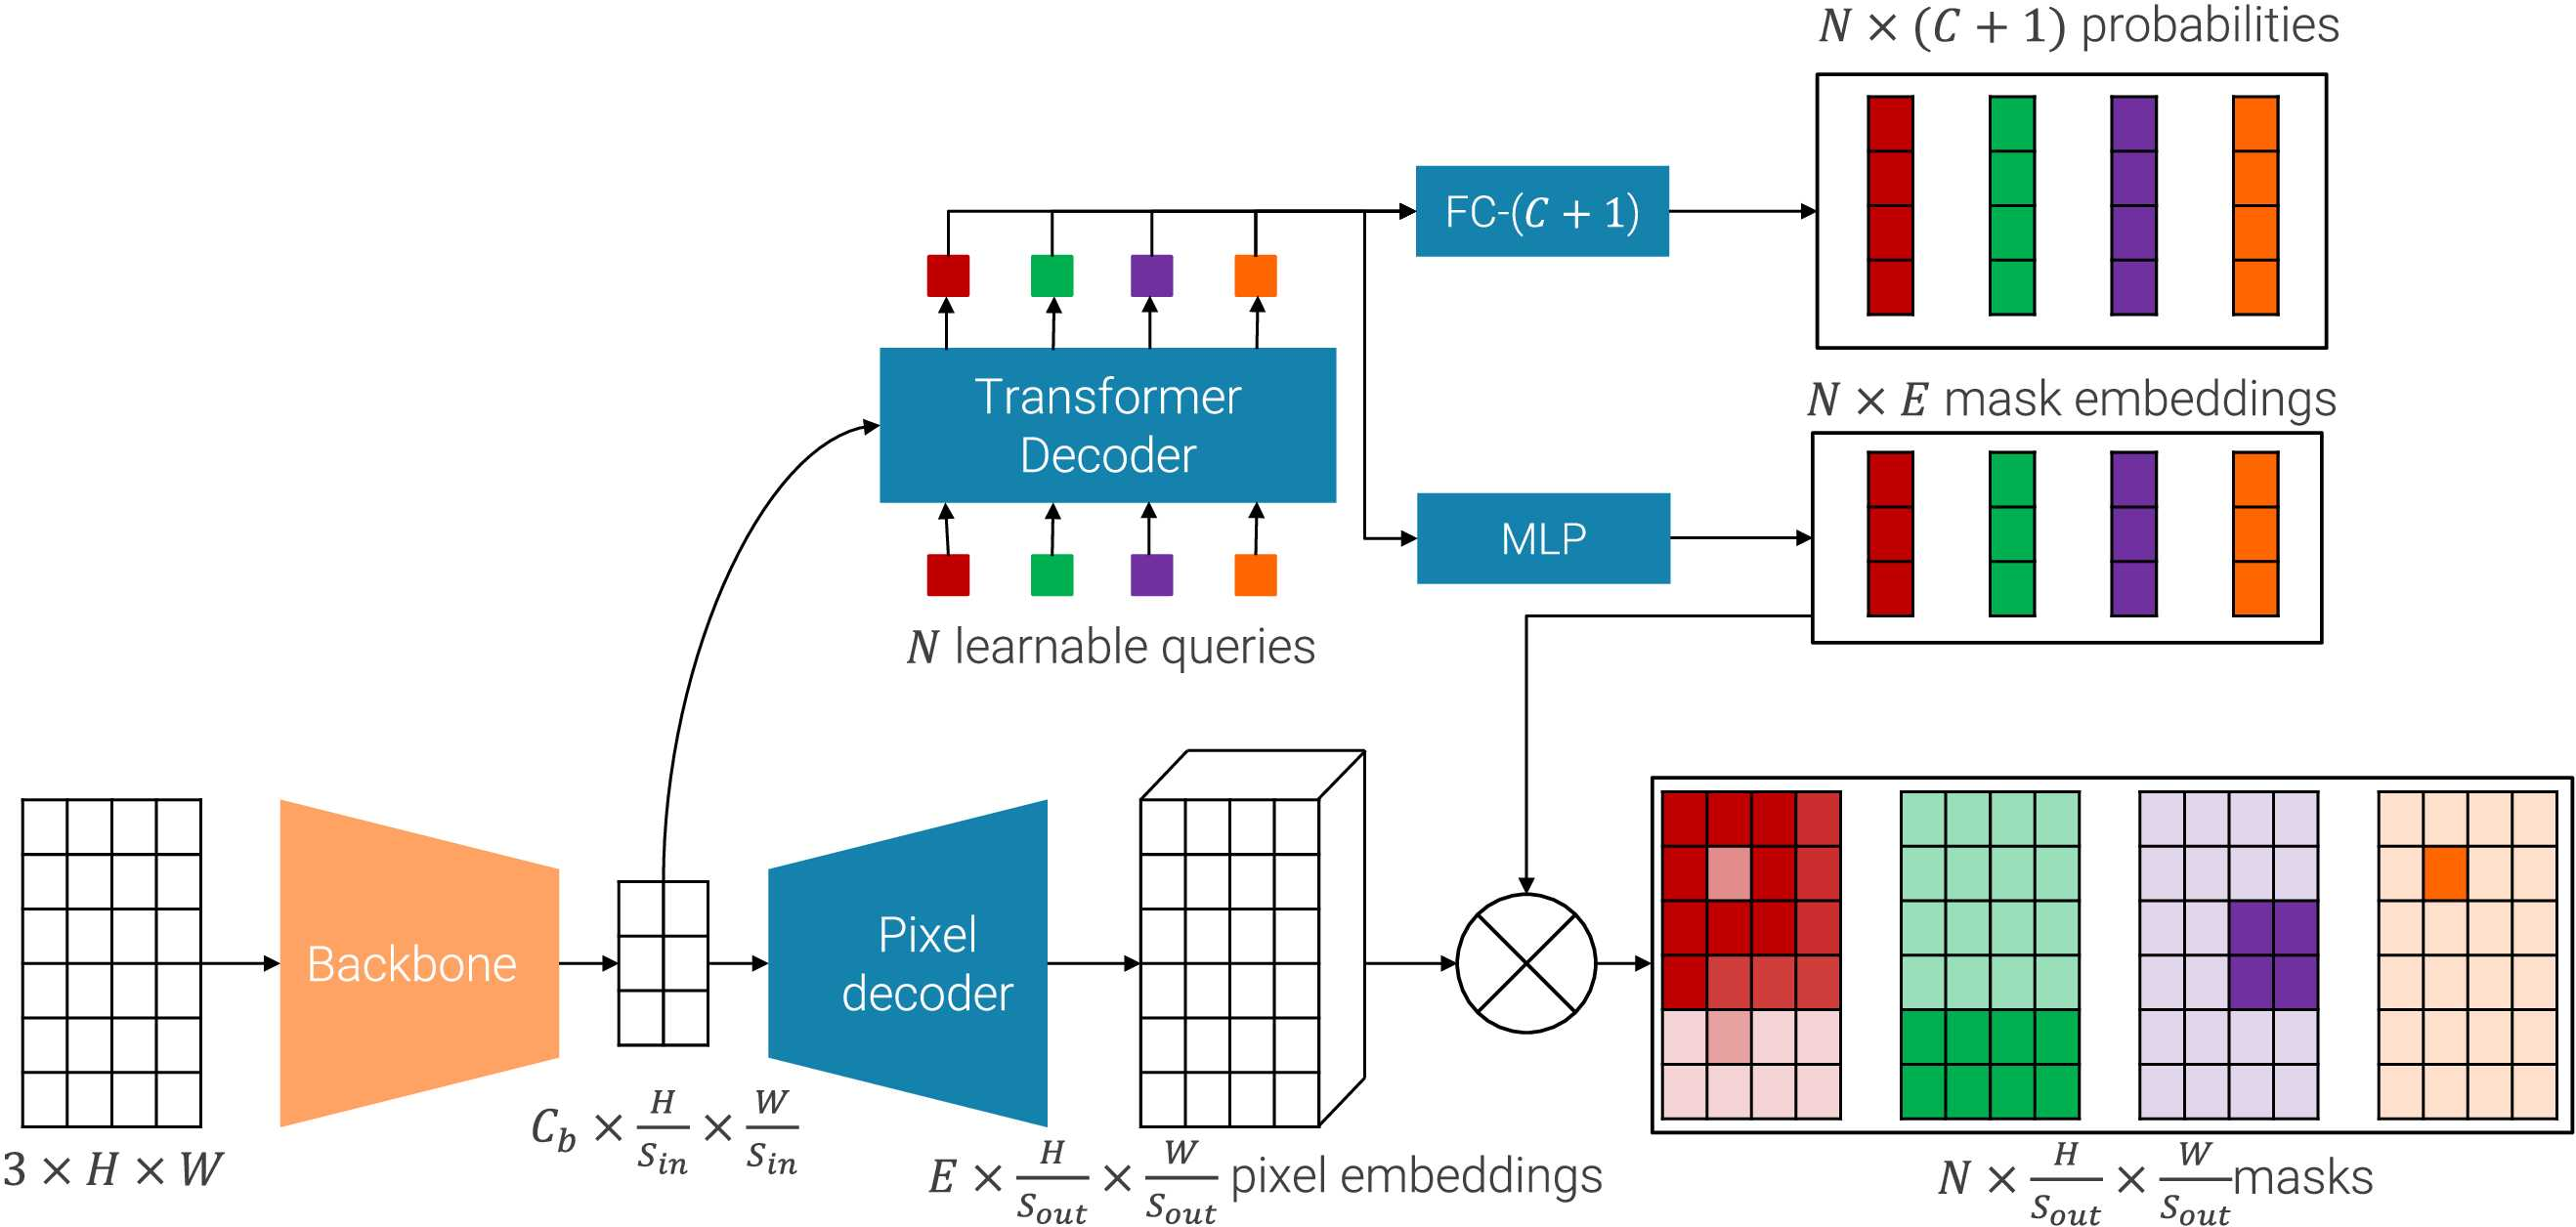
\includegraphics[width=0.75\linewidth]{./img/_maskformer_decoder.jpg}
                \end{figure}

            \item[Inference]
                Given the output class probabilities $\vec{p}_1, \dots, \vec{p}_N$ and masks $\matr{m}_1, \dots, \matr{m}_N$, inference is done as follows:
                \begin{enumerate}
                    \item Determine the class $c_i$ of the $i$-th mask from the distribution $\vec{p}_i$.
                    \item Classify each pixel $(u, v)$ as follows:
                    \begin{enumerate}
                        \item For each mask $i$ that is not background, compute the following score:
                        \[ s_i = \vec{p}_i(c_i) \cdot \matr{m}_i(u, v) \]
                        \item Select the mask with the highest score $s_i$ as the one associated to the pixel.
                    \end{enumerate}
                \end{enumerate}

                \begin{remark}
                    Up-sampling might be needed to match the shape of the mask to the original image.
                \end{remark}

                \begin{figure}[H]
                    \centering
                    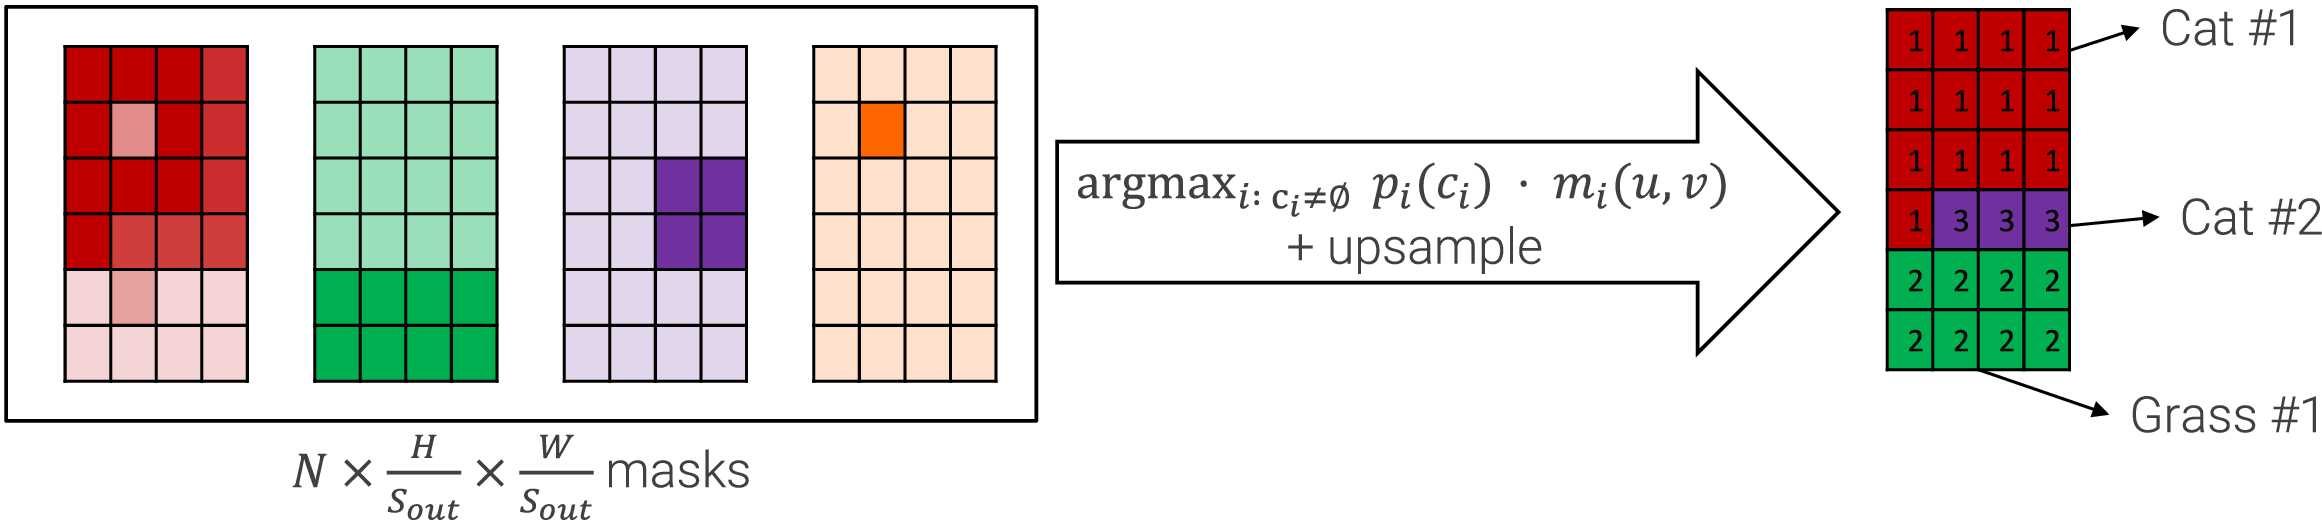
\includegraphics[width=0.8\linewidth]{./img/_maskformer_inference.jpg}
                \end{figure}
        \end{description}

    \begin{remark}
        Although it is able to solve all types of segmentation, MaskFormer does not have state-of-the-art results and it is hard to train.
    \end{remark}
\end{description}


\subsection{Masked-attention mask transformer (Mask2Former)}

\begin{description}
    \item[Mask2Former] \marginnote{Mask2Former}
        Modification of MaskFormer with the addition of:
        \begin{itemize}
            \item Masked attention in the transformer decoder for faster training and better results.
            \item Multi-scale high-resolution features in the pixel-decoder for multi-scale detection.
            \item Training speed-up by not supervising all pixels (i.e., not all pixels of the mask are trained at once, like a sort of dropout).
        \end{itemize}

        \begin{figure}[H]
            \centering
            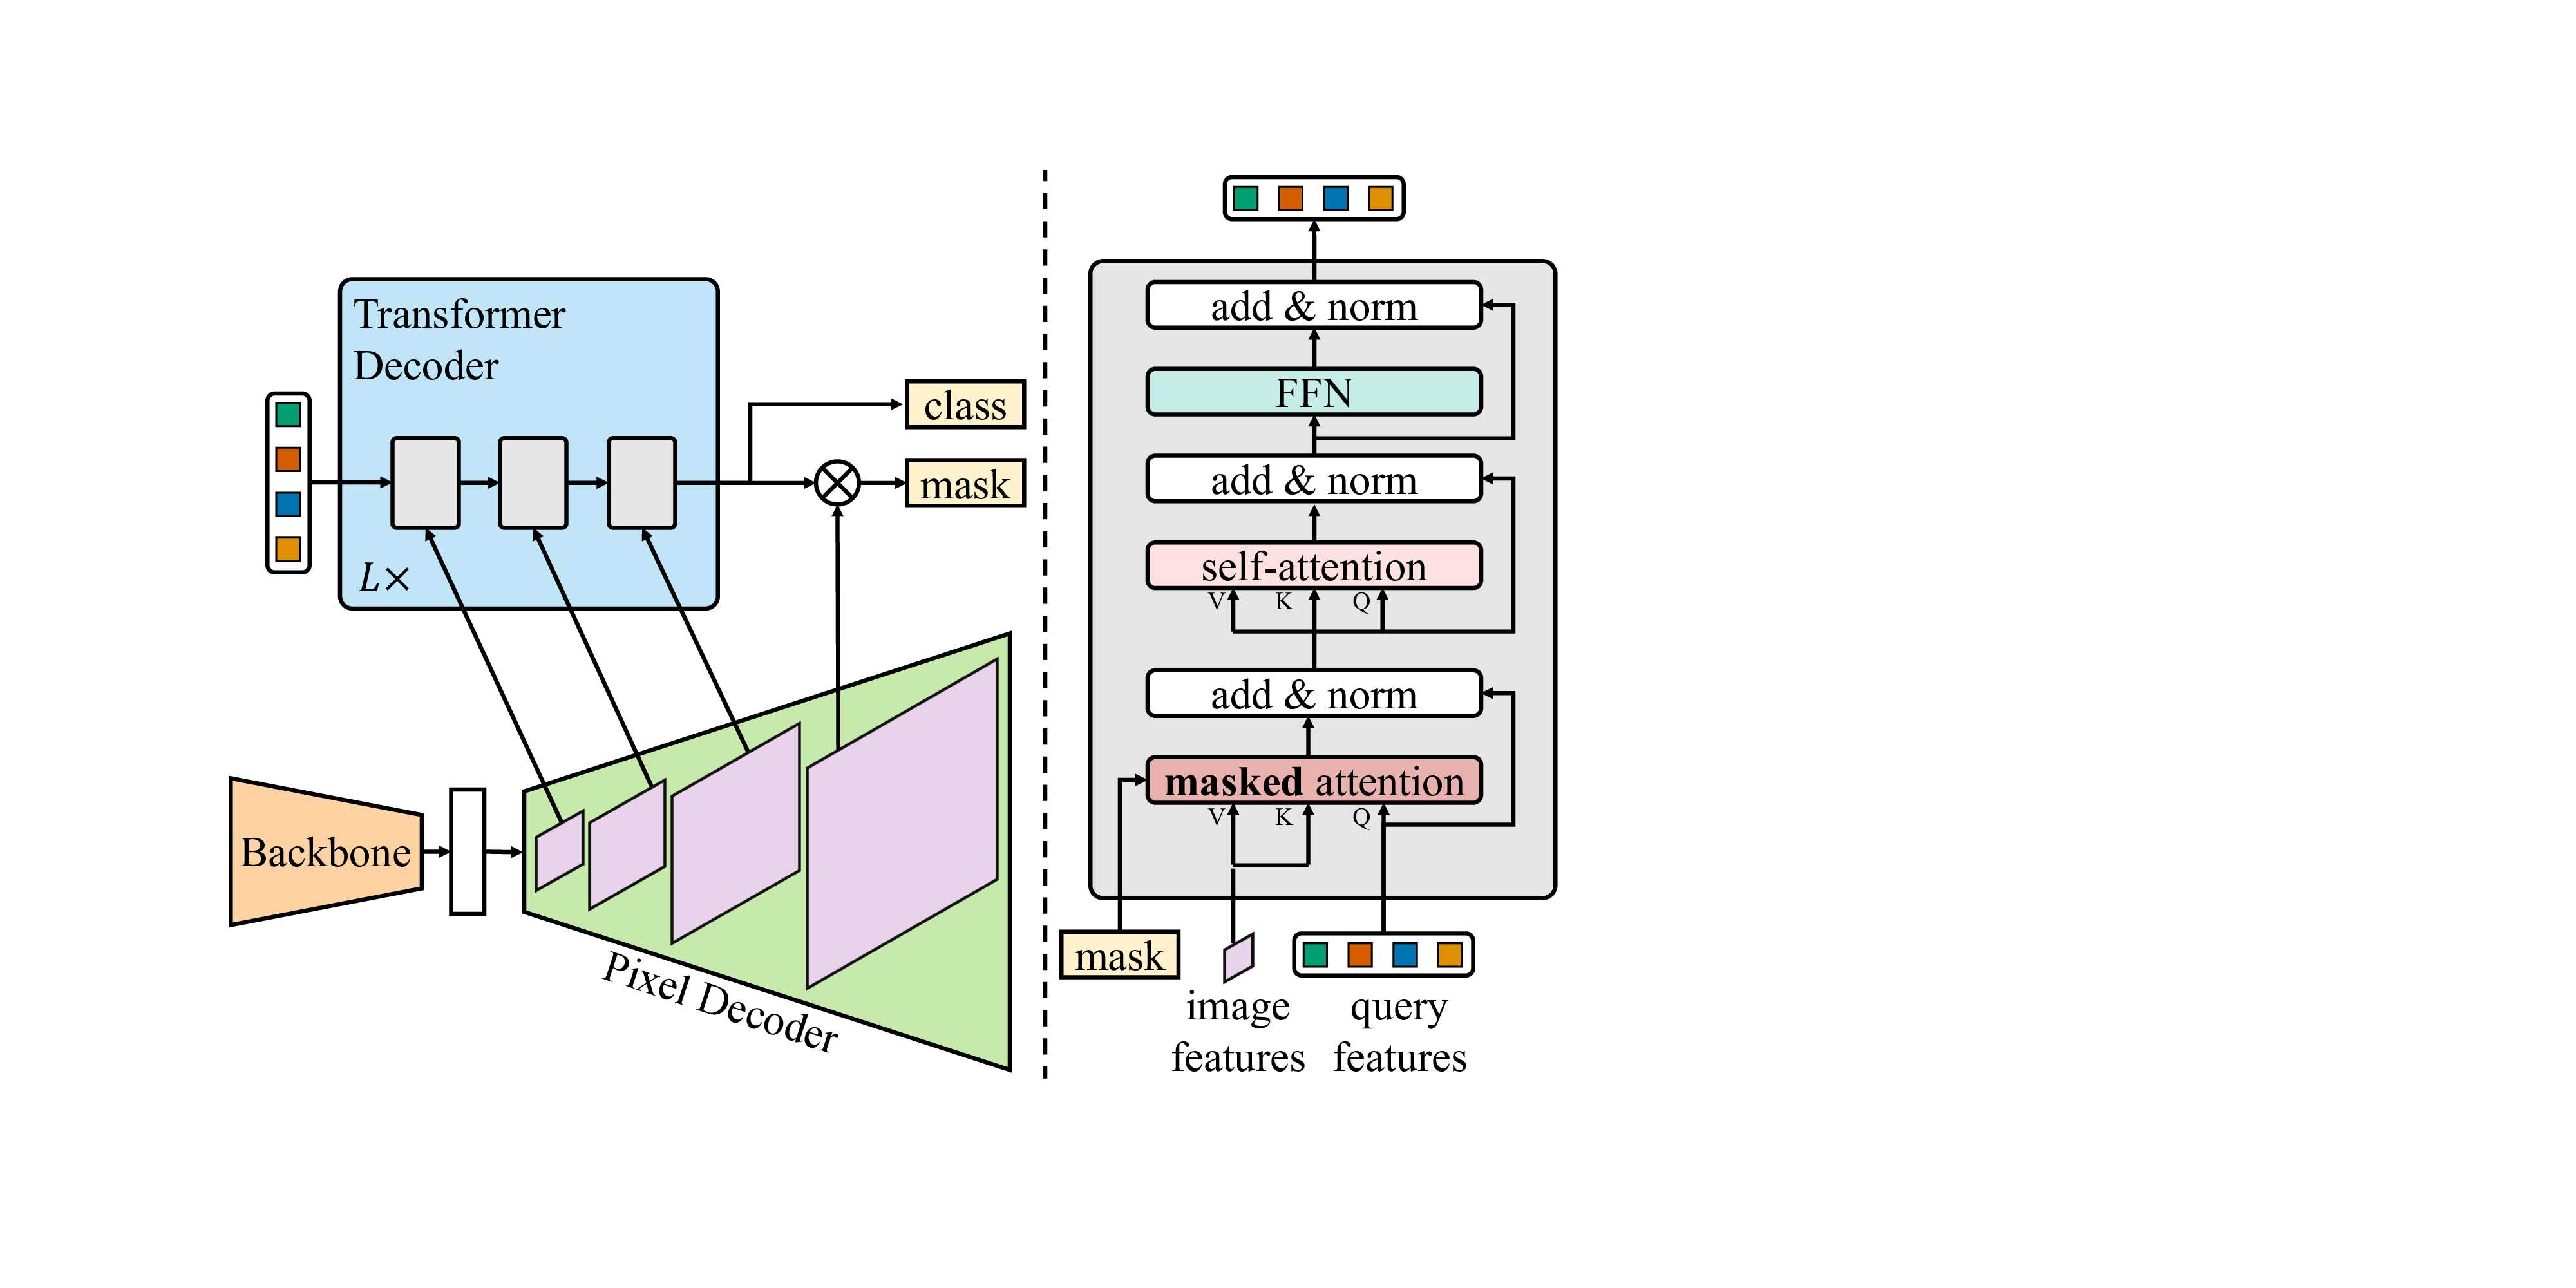
\includegraphics[width=0.45\linewidth]{./img/_mask2former.jpg}
        \end{figure}
\end{description}



\begin{subappendices}

\section{Appendix: Spatial pyramid pooling layer}
    \begin{description}
        \item[Spatial pyramid pooling layer (SPP)] \marginnote{Spatial pyramid pooling layer (SPP)}
            Method to obtain a representation with a fixed-resolution containing different scales.

            The input image is first passed through the CNN backbone. Then, the feature map is max-pooled with a fixed number of variable-size windows before being flattened.

            \begin{remark}
                This can be seen as an extension of global average pooling to preserve spatially localized information.
            \end{remark}

            \begin{figure}[H]
                \centering
                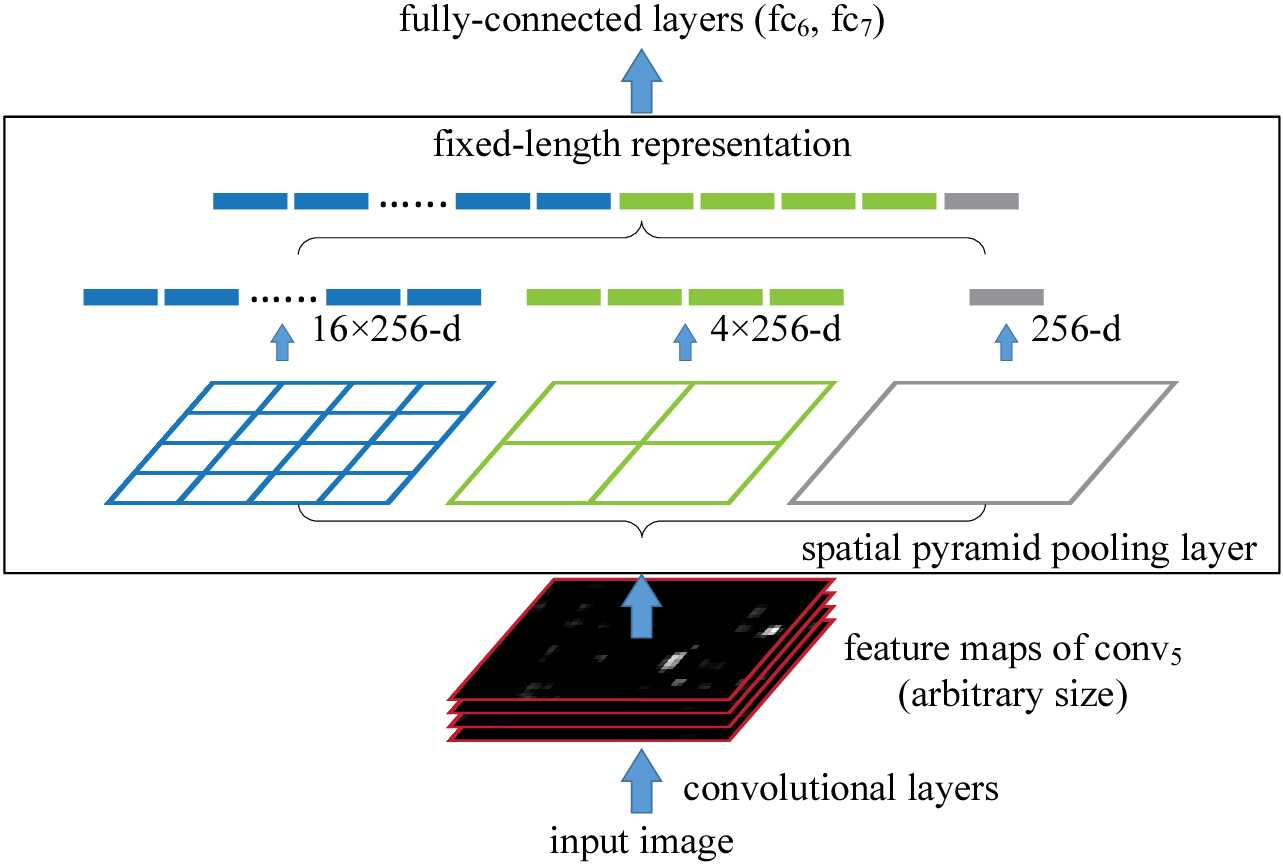
\includegraphics[width=0.5\linewidth]{./img/_spp.jpg}
            \end{figure}
    \end{description}


    \subsection{DeepLab v2 ASPP}

    ASPP in DeepLab v2 emulates SPP through dilated convolutions with increasing rate that are concatenated and aggregated through a $1 \times 1$ convolution.

    \begin{figure}[H]
        \centering
        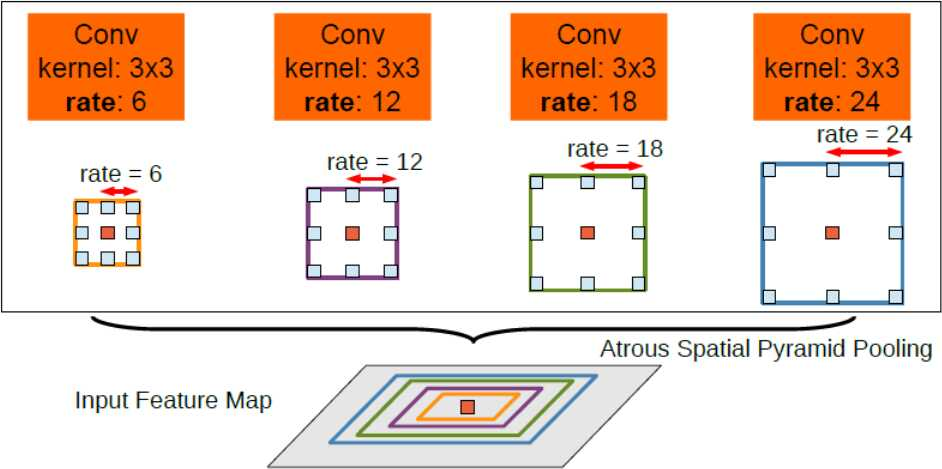
\includegraphics[width=0.5\linewidth]{./img/aspp_deeplabv2.jpg}
    \end{figure}

    \begin{remark}
        When the dilation rate grows, the actual number of relevant weights that are not applied to the padding decreases.

        \begin{figure}[H]
            \centering
            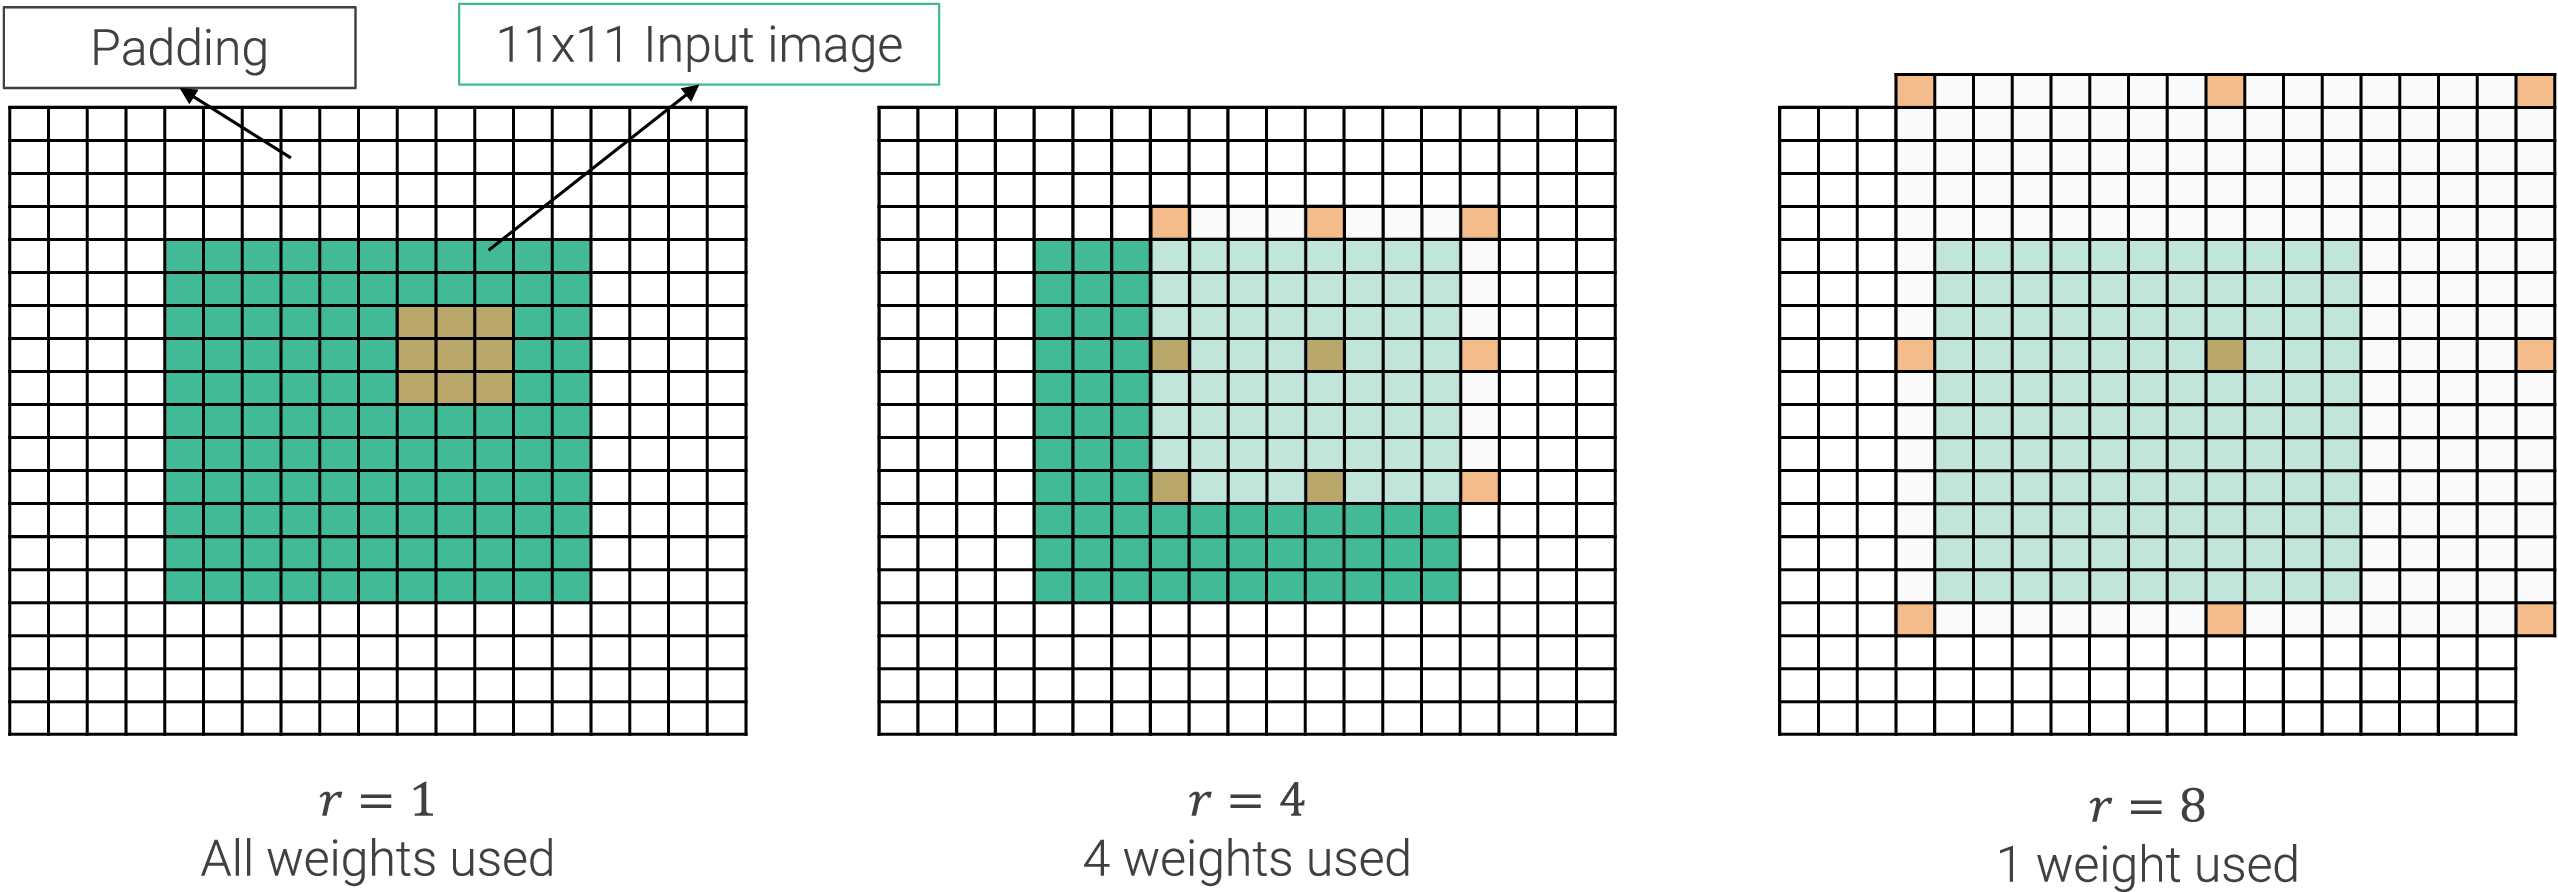
\includegraphics[width=0.8\linewidth]{./img/_dilated_conv_weights.jpg}
        \end{figure}
    \end{remark}


    \subsection{DeepLab v3 ASPP}

    ASPP on DeepLab v3 is formed by dilated convolutions and a path that computes global image features to emulate larger dilation rates (i.e., avoid wasting computation on padding with dilated convolutions with a large rate).

    \begin{figure}[H]
        \centering
        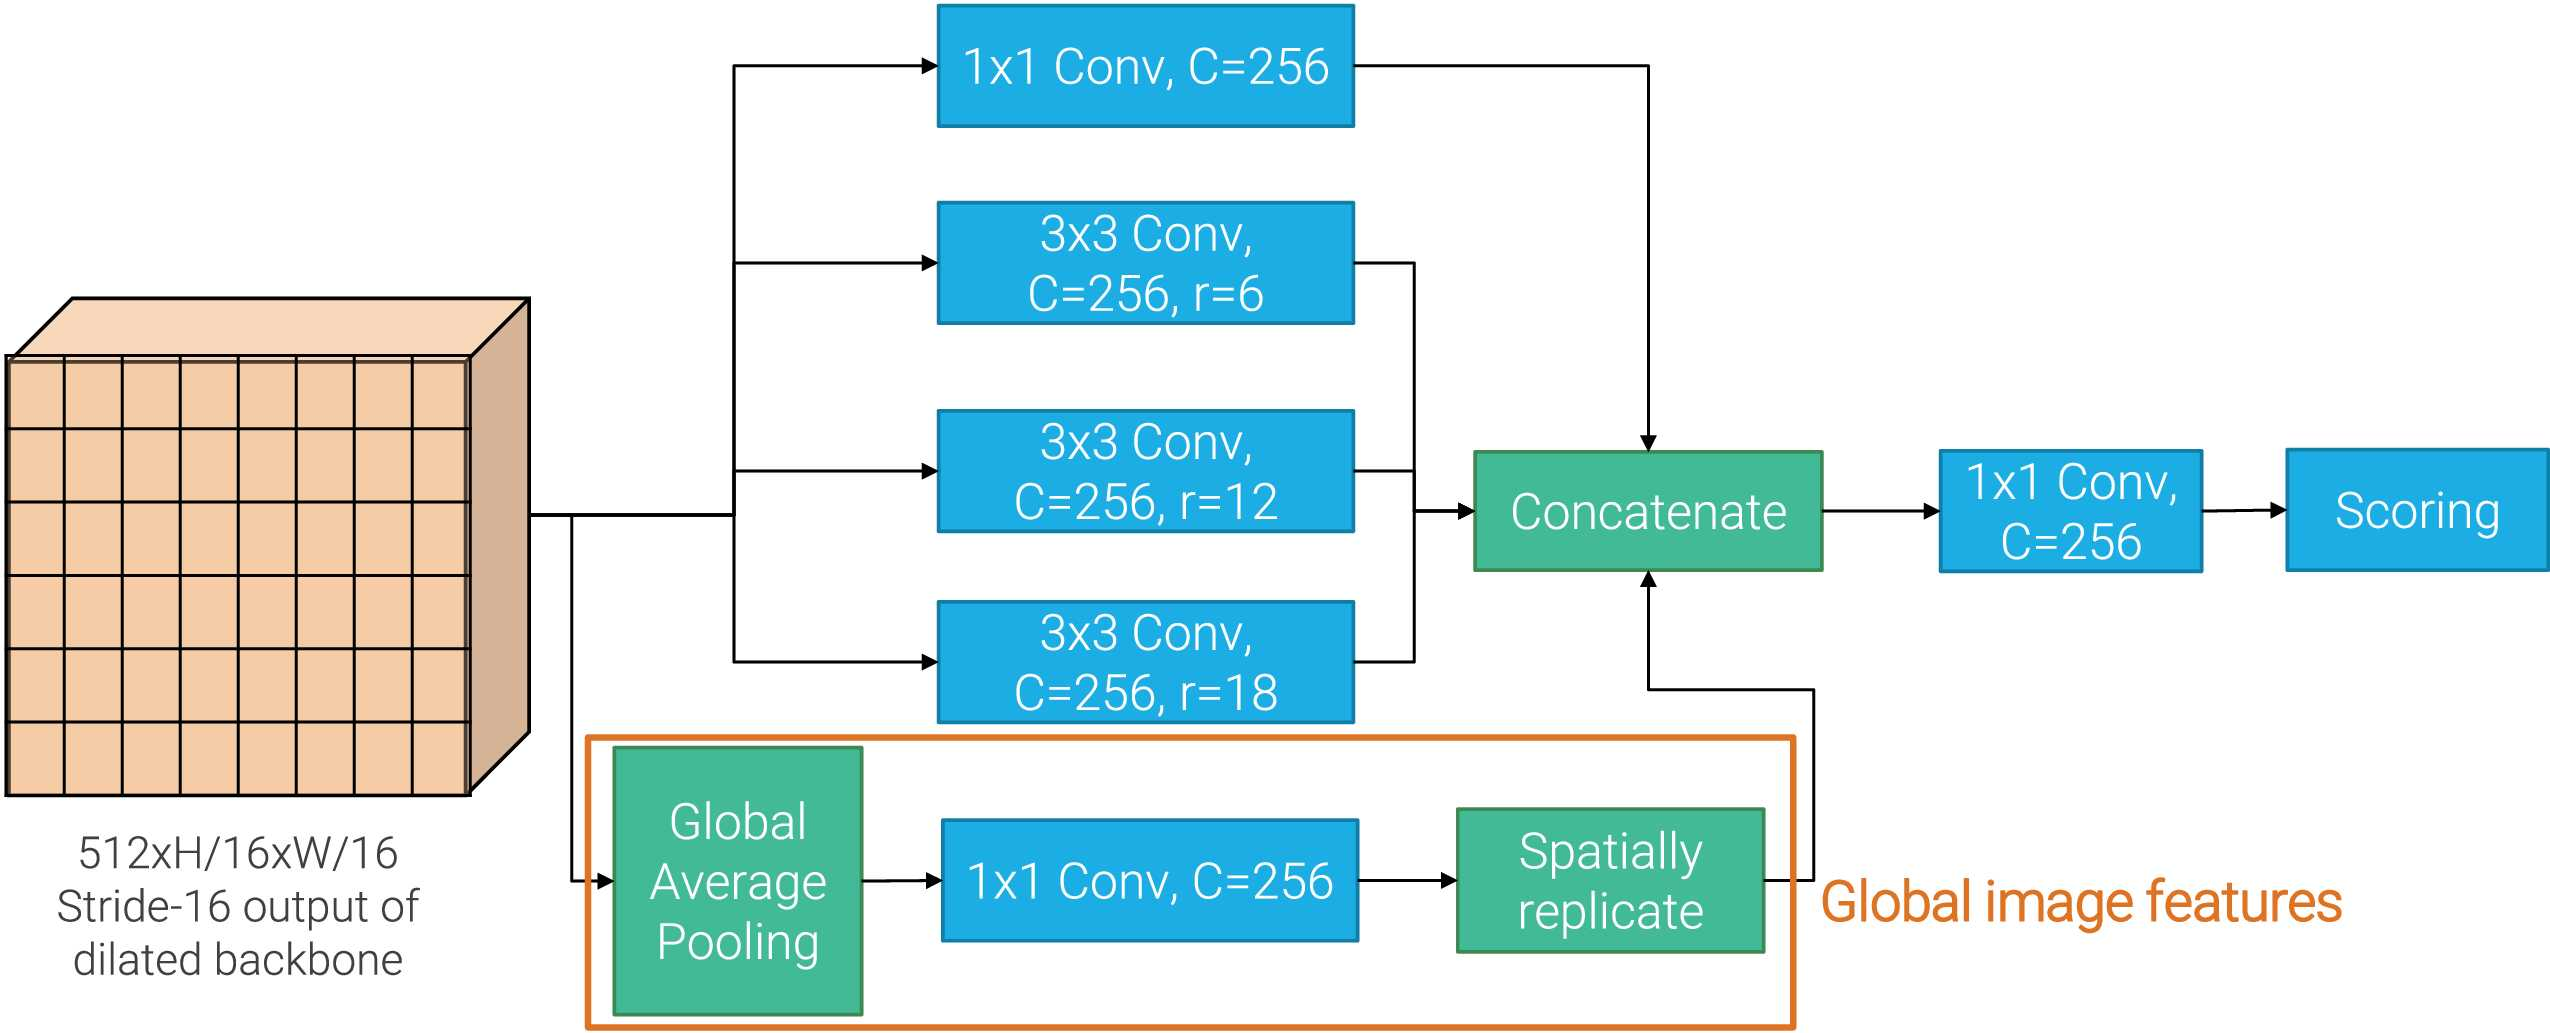
\includegraphics[width=0.75\linewidth]{./img/_deeplabv3_aspp.jpg}
        \caption{
            ASPP with stride-16. With stride-8, rates are doubled.
        }
    \end{figure}
\end{subappendices}
